\documentclass[11pt,a4paper]{article}
\usepackage[margin=25mm]{geometry}
\usepackage{amsmath,amssymb,amsthm,mathtools,booktabs,tikz,hyperref}
\usepackage{microtype}
\usepackage{mathrsfs,tikz-cd}
\providecommand{\tightlist}{\setlength{\itemsep}{0pt}\setlength{\parskip}{0pt}}
\usetikzlibrary{arrows.meta,positioning}
\newtheorem{theorem}{Theorem}[section]
\newtheorem{proposition}[theorem]{Proposition}
\newtheorem{lemma}[theorem]{Lemma}
\theoremstyle{definition}\newtheorem{definition}[theorem]{Definition}
\newtheorem{remark}[theorem]{Remark}
\newcommand{\Z}{\mathbb Z}\newcommand{\Q}{\mathbb Q}
\newcommand{\C}{\mathbb C}\newcommand{\R}{\mathbb R}
\newcommand{\B}{\mathbb B}\newcommand{\N}{\mathbb N}
\newcommand{\F}{\mathbb F}
\newcommand{\Spec}{\operatorname{Spec}}\newcommand{\SpecMon}{\operatorname{Spec}_{\mathrm{mon}}}
\newcommand{\SpecLat}{\operatorname{Spec}_{\mathrm{lat}}}
\newcommand{\supp}{\operatorname{supp}}\newcommand{\tr}{\operatorname{tr}}
\newcommand{\Sch}{\mathcal S}\newcommand{\im}{\operatorname{im}}
\newcommand{\rk}{\operatorname{rank}}\newcommand{\cl}{\operatorname{cl}}
\newcommand{\Pp}{\mathcal P}\newcommand{\LL}{\mathcal L}
\newcommand{\G}{\mathsf G}\newcommand{\Tor}{\operatorname{Tor}}\newcommand{\Frac}{\operatorname{Frac}}
\newcommand{\RZ}{\operatorname{RZ}}\newcommand{\Ann}{\operatorname{Ann}}
\newtheorem{corollary}[theorem]{Corollary}

\providecommand{\Hom}{\operatorname{Hom}}
\providecommand{\Ext}{\operatorname{Ext}}
\providecommand{\RHom}{\operatorname{RHom}}
\providecommand{\coker}{\operatorname{coker}}
\providecommand{\Sh}{\operatorname{Sh}}
\providecommand{\Ab}{\operatorname{Ab}}
\providecommand{\length}{\operatorname{length}}
\providecommand{\PP}{\mathcal P}

\title{Split Zero and the Arithmetic Trace\\A reconstruction from the complete support geometry}
\author{Split-Zero research programme}
\date{23 September 2026; edition SZ-20260922-031}
\begin{document}
\maketitle
This manuscript constructs the programme from its coefficient operations, all relevant prime spectra, and the maps connecting them. Every assertion below has its stated mathematical scope. The manuscript is being written cumulatively; it does not assert completion of the RH argument or of the entire requested reconstruction.
\tableofcontents

% BEGIN COMPLETE PROOF SOURCE: 01_spectra.tex
\section{The coefficient operations and their prime spectra}
\label{sec:rebuilt-spectra}
\begin{definition}
For a nonzero commutative unital ring $R$, let $G(R)=R\sqcup\{\tau\}$. Supported elements have their original ring sum and product; $x+\tau=x$ and $x\tau=\tau$. Write $e=0_R$ for the supported zero. Thus $e\ne\tau$, $e^2=e$, and $er=e$ for every supported $r$.
\end{definition}
The injection $\tau\mapsto(0,0)$, $r\mapsto(r,1)$ into $R\times\B$ proves all semiring laws, including distributivity. Here addition in $\B$ is join and multiplication is meet. The two projections are
\begin{equation}\label{eq:base-two-maps}
 p:G(R)\to R,\quad p(\tau)=0,\ p(r)=r;
 \qquad \chi:G(R)\to\B,\quad\chi(\tau)=0,\ \chi(r)=1.
\end{equation}
They jointly retain the entire original element. Every map to a ring kills $e$ since $e+e=e$, and then factors uniquely through $p$. The supported inclusion of $R$ does not preserve the specified additive zero and is not a semiring section of $p$.

\begin{theorem}[The scalar spectrum and its stalks]\label{thm:rebuilt-scalar}
The ideals of $G(R)$ are $\{\tau\}$ and $J\cup\{\tau\}$ for ring ideals $J$. Its primes are
\[
 P_\tau=\{\tau\},\qquad P_{\mathfrak p}=\mathfrak p\cup\{\tau\}\quad(\mathfrak p\in\Spec R).
\]
The map induced by $p$ identifies $\Spec R$ with $V(e)$, while $D(e)=\{P_\tau\}$ is open and dense. The localization stalks are
\[
 G(R)_{P_\tau}=\B,\qquad G(R)_{P_{\mathfrak p}}=G(R_{\mathfrak p}).
\]
For $R=\Z$, all strict maximal prime chains are
\begin{equation}\label{eq:scalar-chain}
 \{\tau\}\subsetneq\{\tau,e\}\subsetneq p\Z\cup\{\tau\}.
\end{equation}
In particular its dimension is two.
\end{theorem}
\begin{proof}
Every ideal contains $\tau$. If an ideal contains a supported element, multiplication by $e$ places $e$ in the ideal. Its supported intersection is a ring ideal because multiplication by $-1$ supplies additive inverses. This proves the ideal classification and its converse. A product equals $\tau$ only if a factor does, proving primality of $P_\tau$. Testing supported products proves primality of $J\cup\{\tau\}$ exactly when $J$ is prime.

For supported $a$, $D(a)=\{P_\tau\}\cup D_R(a)$, whereas $D(\tau)$ is empty. These formulas prove the topology assertions, and $P_\tau$ is contained in every prime. At $P_\tau$, every supported element is inverted, including $e$. Its idempotence forces $e=1$, and $er=e$ then forces every supported $r$ to equal $1$. The character $\chi$ factors through the localization and distinguishes $1$ from $\tau$, proving that the result is exactly $\B$. At $P_{\mathfrak p}$ the denominators are $R\setminus\mathfrak p$. The fraction map $r/s\mapsto r/s$, $\tau/s\mapsto\tau$ is an isomorphism: equality of supported fractions is precisely the usual localization relation; an absent fraction cannot equal a supported fraction since denominators and the extra multiplier remain supported. The list of ring primes of $\Z$ now proves \eqref{eq:scalar-chain} and excludes longer chains.
\end{proof}

\begin{proposition}[The direction of the absolute-point maps]\label{prop:base-arrows}
The maps in \eqref{eq:base-two-maps} induce
\[
 \Spec R\xrightarrow{\text{closed}}\Spec G(R)
 \xleftarrow{\text{open}}\Spec\B.
\]
There is no unital semiring map $\B\to G(R)$. The pointed multiplicative monoid $\{0,1\}$ does map to the multiplicative monoid of $G(R)$ by $0\mapsto\tau$, $1\mapsto1$.
\end{proposition}
\begin{proof}
The first assertion is the localization and prime contraction already proved. A map from $\B$ would send $1+1=1$ to $1_R+1_R=1_R$, which contradicts $1_R\ne0_R$. The two-element pointed monoid has no such additive relation, and its product table verifies the last map. Thus the two arrows and the pointed-monoid map retain their exact categories.
\end{proof}

\subsection{Every multiplicative prime, before imposing addition}
Let $M$ be the pointed multiplicative monoid underlying $G(\Z)$ and let $\mathcal P$ be the rational primes. A monoid ideal is absorbing under multiplication; no additive closure is required.
\begin{theorem}[The complete monoid spectrum]\label{thm:rebuilt-monoid}
For $\Sigma\subseteq\mathcal P$, put
\[
 J_\Sigma=\{\tau,e\}\cup\{n\in\Z\setminus\{0\}:p\mid n\text{ for some }p\in\Sigma\}.
\]
Then
\[
 \SpecMon M=\{\{\tau\}\}\sqcup\{J_\Sigma:\Sigma\subseteq\mathcal P\},
 \qquad J_\Sigma\subseteq J_{\Sigma'}\iff\Sigma\subseteq\Sigma'.
\]
This spectrum has infinite dimension. The map
\begin{equation}\label{eq:semiring-monoid-inclusion}
 j:\Spec G(\Z)\longrightarrow\SpecMon M
\end{equation}
that keeps each prime ideal as a subset is a continuous topological embedding. Its image is exactly $\{\tau\}$, $J_\varnothing$, and the $J_{\{p\}}$.
\end{theorem}
\begin{proof}
The displayed sets are proper absorbing ideals. Products in $J_\Sigma$ either involve $\tau$, vanish in the integral domain $\Z$, or have a prime factor in $\Sigma$, so they satisfy primality. If a prime monoid ideal contains a supported element it contains $e$. It contains neither unit $1,-1$. Every nonzero element in it has an integer prime factor in it, by repeated primality and integer factorization. Conversely it contains every multiple of every such prime factor. This proves exhaustion, including $J_\varnothing=\{\tau,e\}$. Membership of a rational prime $p$ tests whether $p\in\Sigma$, proving the inclusion statement. Arbitrarily long strictly nested finite subsets give arbitrarily long prime chains.

The scalar theorem identifies the image of $j$. For every $a\in M$, the inverse image under $j$ of the monoid basic open $D_M(a)$ is the semiring basic open $D_{G(\Z)}(a)$. These basics also generate the topology on the source, proving that the injection is an embedding. Finally if $\Sigma$ contains distinct primes $p,q$, B\'ezout integers $u,v$ give $up+vq=1$. Both summands belong to $J_\Sigma$, so additive closure would force $1$ into it. Such a monoid prime therefore cannot be a semiring prime. This also proves exactly which additive relation removes it.
\end{proof}

\begin{proposition}[Reconstruction retains the missing relations]\label{prop:preaddition-rebuild}
Let $\N_0[M]$ be the monoid semiring with the basis symbol $[\tau]$ identified with its additive zero. Then the quotient by
\[
 [a]+[b]\sim[a+b]\qquad(a,b\in\Z)
\]
is canonically $G(\Z)$.
\end{proposition}
\begin{proof}
Evaluation $[a]\mapsto a$ respects all displayed relations. Every nonempty supported sum reduces to the single basis symbol of its integer sum, while the empty sum remains the symbol $\tau$. Conversely $a\mapsto[a]$, $\tau\mapsto0$ preserves multiplication, every supported addition, and addition with the specified zero. These maps are inverse. The contraction of $[\tau]$ is essential: in the uncontracted free semiring, the relations $[x]+[\tau]=[x]$ alone do not identify $[\tau]$ with the empty sum. Indeed they hold in the semiring obtained by adjoining another external zero below the already specified zero of $G(\Z)$, where the two remain distinct. This gives an explicit separating model for the missing relation.
\end{proof}

\subsection{The complete lattice of zero-amplitude support}
Let $L$ be a nontrivial bounded distributive lattice and put
\[
 S_L=G_L(R)=\{(0,\lambda):\lambda\in L\}\cup\{(r,1_L):r\in R\}
 \subset R\times L.
\]
Operations are $(r,\lambda)+(s,\mu)=(r+s,\lambda\vee\mu)$ and
$(r,\lambda)(s,\mu)=(rs,\lambda\wedge\mu)$. Set $z_\lambda=(0,\lambda)$, $\tau_L=z_0$, $e_L=z_1$, and $Z_L=\{z_\lambda\}$.
\begin{theorem}[All support and arithmetic primes]\label{thm:rebuilt-full-support}
The primes of $S_L$ are exactly
\[
 P_{\mathfrak a}=\{z_\lambda:\lambda\in\mathfrak a\},\quad\mathfrak a\in\SpecLat L;
 \qquad Q_{\mathfrak p}=Z_L\cup\{(r,1):r\in\mathfrak p\},\quad\mathfrak p\in\Spec R.
\]
Within each family, inclusions retain the original prime order; every $P_{\mathfrak a}$ is strictly contained in every $Q_{\mathfrak p}$. Topologically
\begin{equation}\label{eq:full-spectral-base}
 \Spec S_L=\SpecLat L\blacktriangleright\Spec R,
 \qquad D(e_L)=\SpecLat L,\quad V(e_L)=\Spec R,
\end{equation}
where opens are opens of the first stratum and sets consisting of that entire stratum together with an open of the second. If both dimensions are finite, their dimensions add with one further step between the strata.
\end{theorem}
\begin{proof}
An ideal containing a supported element contains $e_L$ by multiplication by it and therefore all of $Z_L$, since $e_Lz_\lambda=z_\lambda$. Its supported elements form a ring ideal. Every remaining ideal is $\{z_\lambda:\lambda\in\mathfrak a\}$ for a proper lattice ideal: closure under join follows from addition, and downward closure follows from multiplication by $z_\mu$ for $\mu\le\lambda$. Conversely these are all ideals. Primality in the first family is the meet-prime condition on $\mathfrak a$; in the second it is the ring-prime condition. Products involving a zero-fibre element obey exactly these tests. The inclusions follow from the displayed sets. Finally
\[
 D(z_\lambda)=\{P_{\mathfrak a}:\lambda\notin\mathfrak a\},\qquad
 D((r,1))=\SpecLat L\cup D_R(r)
\]
prove the topology and the two strata. Every chain is a support chain followed by an arithmetic chain, and maximal finite chains concatenate, proving the dimension formula.
\end{proof}

\begin{proposition}[Two support channels and their exact comparison]\label{prop:two-support-branches}
For $L=\mathcal P(\{1,2\})$, $\{\tau_L\}$ is not prime, since $z_{\{1\}}z_{\{2\}}=\tau_L$ although neither factor is absent. There are two support primes
\[
 P_1=\{\tau_L,z_{\{2\}}\},\qquad P_2=\{\tau_L,z_{\{1\}}\}.
\]
For $R=\Z$, each specializes to the common $Q_{(0)}$ and then to every $Q_{(p)}$. Moreover
\begin{equation}\label{eq:common-amplitude-fibre-product}
 G_{\B^2}(R)\simeq G(R)\mathbin{\times_R}G(R),
\end{equation}
where the two maps to $R$ are ring reflections. The two factor-generic primes contract to $P_1,P_2$, while their arithmetic primes above the same $\mathfrak p$ both contract to $Q_{\mathfrak p}$.
\end{proposition}
\begin{proof}
The two coordinate maps $L\to\B$ have precisely the displayed prime kernels; a proper prime ideal must contain exactly one of the two atoms, proving exhaustion. For \eqref{eq:common-amplitude-fibre-product}, send $z_A$ to the pair with entry $e$ on $A$ and $\tau$ off $A$, and send $(r,\{1,2\})$ to $(r,r)$. Equal nonzero amplitudes force both coordinates to be that supported value, whereas common amplitude zero allows exactly the four masks. Hence the map is onto the fibre product and injective; the operations verify it is an isomorphism. Taking inverse images of the factor primes proves their contractions.
\end{proof}

\begin{proposition}[What a Boolean branch retains]\label{prop:branch-contraction}
A bounded lattice homomorphism $\epsilon:L\to\B$ induces $\beta_\epsilon:G_L(R)\to G_\B(R)$ by $z_\lambda\mapsto z_{\epsilon(\lambda)}$ and $(r,1)\mapsto(r,1)$. Its spectral image is
\[
 \{P_{\epsilon^{-1}(0)}\}\blacktriangleright\Spec R.
\]
\end{proposition}
\begin{proof}
The map preserves joins, meets and supported arithmetic, hence is a semiring homomorphism. The inverse image of the scalar absent prime is $\{z_\lambda:\epsilon(\lambda)=0\}$, and the inverse image of each arithmetic prime contains the full zero fibre and exactly its original amplitudes. This proves the asserted image. In particular a branch selects one support prime; the formula does not recover the other primes.
\end{proof}

These proofs reconstruct the scalar and multiplicative results of \cite{globalization,secondary} and the lattice-support results of \cite{support}. They give explicit maps whenever their spectra differ. The following section uses the multiplicative prime faces to recover the finite sets of places occurring in the arithmetic trace, retaining the support geometry of \eqref{eq:full-spectral-base} for the cohomological coefficient construction.

% END COMPLETE PROOF SOURCE: 01_spectra.tex


% BEGIN COMPLETE PROOF SOURCE: 04_supported_prime.tex
\section{Supported zero as the central arithmetic prime}
\label{sec:supported-prime}
The nonzero prime element $e$ is part of the starting geometry, not a notation for the semiring zero. The assertion already appears explicitly in \cite[\texttt{thm:zero-prime-not-irr}]{globalization}. Here its ideal, height, localization, quotient, and power filtration are reconstructed on the full lattice-support base.

\begin{theorem}[The supported-zero prime and the arithmetic closed stratum]\label{thm:supported-zero-prime}
Let $R$ be a nonzero integral domain and $L$ a nontrivial bounded distributive lattice. In $S=G_L(R)$ the supported zero $e=z_1$ is a nonzero nonunit prime element. Precisely,
\begin{equation}\label{eq:e-divisibility}
 eS=Z_L=\ker p_L=:E,\qquad
 e\mid x\ \Longleftrightarrow\ p_L(x)=0,\qquad
 e\mid xy\ \Longrightarrow\ e\mid x\text{ or }e\mid y.
\end{equation}
Its principal ideal $E$ is prime, $E^2=E$, and it is not irreducible because $e=e\cdot e$ with neither factor a unit. Every support prime lies strictly below $E$. The primes above $E$ are exactly the arithmetic primes $Q_{\mathfrak p}$, and
\[
 V(E)\simeq\Spec R.
\]
For finite-dimensional $\SpecLat L$,
\[
 \operatorname{ht}(E)=\dim\SpecLat L+1.
\]
For $R=\Z$ and finite Boolean $L=\B^I$ with $I\ne\varnothing$, $E$ has height one and each $Q_{(p)}$ has height two.
\end{theorem}
\begin{proof}
For $z_\lambda\in Z_L$, $ez_\lambda=z_\lambda$, so every zero-amplitude element belongs to $eS$. Conversely a product with $e$ has zero amplitude, proving the first equality and the divisibility equivalence. Since $R$ is a domain, $p_L(x)p_L(y)=0$ implies that one factor has zero amplitude; this proves the prime-element condition and primality of its ideal. The element $e$ differs from $\tau=z_0$, and it is not a unit since every product with it has amplitude zero, whereas $1$ has nonzero amplitude. Its idempotence proves both $E^2=E$ and the failure of irreducibility.

The complete prime classification places every support prime below $Q_{(0)}=E$, and a domain has no arithmetic prime strictly below $(0)$. Thus every chain ending at $E$ consists of a support chain followed by this final step. Taking suprema of lengths proves the height formula. A finite Boolean lattice has only its coordinate prime ideals, which are pairwise incomparable: primality and disjointness of atoms force exactly one atom outside a prime ideal. Its lattice spectrum has dimension zero, proving the last assertions.
\end{proof}

\begin{theorem}[The stalk and residue at the supported-zero prime]\label{thm:e-stalk}
If $K=\operatorname{Frac}R$, then
\begin{equation}\label{eq:e-localization}
 S_E\simeq G_L(K),\qquad S_E/E S_E\simeq K.
\end{equation}
The first map retains every support element $z_\lambda$; the second is the ring reflection and uses the ideal's Bourne congruence. Inverting the element $e$, in contrast, gives
\begin{equation}\label{eq:e-element-localization}
 S[e^{-1}]\simeq L.
\end{equation}
\end{theorem}
\begin{proof}
The complement of $E$ consists exactly of supported nonzero amplitudes. Inverting them creates their original field fractions. For a zero-fibre element, multiplication by any such denominator fixes $z_\lambda$, so its fraction still equals the same $z_\lambda$. Different zero-fibre labels remain distinct: the support map $S\to L$ sends every denominator to $1$ and therefore distinguishes them in the localization. A nonzero field fraction cannot become a zero-fibre element because the ring-reflection map to $K$ distinguishes their amplitudes. These observations prove the first isomorphism, including all fraction identifications.

The Bourne relation for $E$ identifies $x,y$ when $x+i=y+j$ for some $i,j\in E$. It preserves amplitudes. Conversely if amplitudes agree, adding $e$ to either element gives the same supported amplitude; hence the relation identifies exactly equal amplitudes. This proves the quotient assertion. For \eqref{eq:e-element-localization}, invertibility of the idempotent $e$ forces $e=1$. Each supported $r$ then satisfies $r=er=e=1$. Every $z_\lambda$ survives, and its inherited join and meet give $L$ with unit $e$. The support map realizes this identification, proving its universal property.
\end{proof}

\begin{proposition}[The complete power filtration of the prime $E$]\label{prop:e-adic}
For every $n\ge1$, $E^n=E$. The ideal-congruence quotients and their inverse limit are
\begin{equation}\label{eq:e-completion}
 S/E^n\simeq R,\qquad \varprojlim_n S/E^n\simeq R.
\end{equation}
Every transition map is the identity on $R$, and the completion map is $p_L$. The support-only ideal $E$ is isomorphic to $L$ with its own multiplicative identity $e$; its inclusion in $S$ is not unit preserving.
\end{proposition}
\begin{proof}
Idempotence $E^2=E$ proves the power identity by induction. The Bourne-quotient argument in the preceding proof applies before localization and identifies $S/E$ exactly with $R$. Thus all levels and transition maps are as stated. The last assertion follows from $z_\lambda z_\mu=z_{\lambda\wedge\mu}$, $z_\lambda+z_\mu=z_{\lambda\vee\mu}$, and $ez_\lambda=z_\lambda$. Since $e\ne1_S$, its internal unit is not the unit of $S$.
\end{proof}

\begin{figure}[ht]
\centering
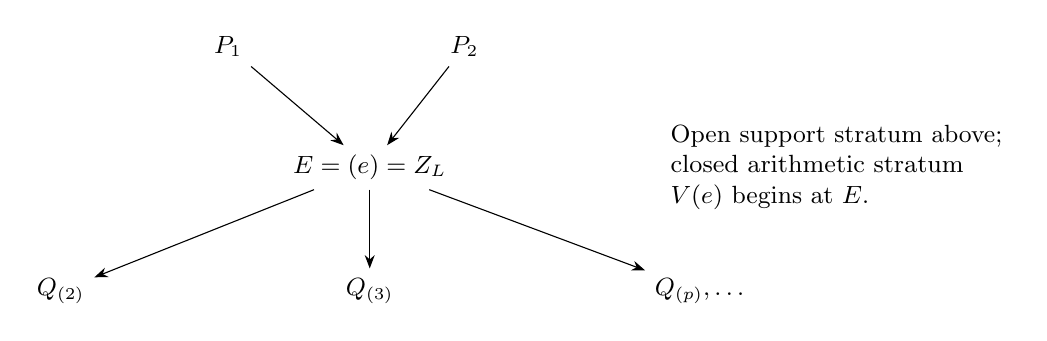
\begin{tikzpicture}[>=Stealth,node distance=10mm and 24mm,every node/.style={font=\small}]
\node (p1) {$P_1$};\node[right=of p1] (p2) {$P_2$};
\node[below=of p1,xshift=18mm] (E) {$E=(e)=Z_L$};
\node[below left=of E] (q2) {$Q_{(2)}$};\node[below=of E] (q3) {$Q_{(3)}$};\node[below right=of E] (qp) {$Q_{(p)},\ldots$};
\draw[->] (p1)--(E);\draw[->](p2)--(E);
\draw[->](E)--(q2);\draw[->](E)--(q3);\draw[->](E)--(qp);
\node[right=26mm of E,text width=43mm] {Open support stratum above;\newline closed arithmetic stratum $V(e)$ begins at $E$.};
\end{tikzpicture}
\caption{Exact specialization diagram for $G_{\B^2}(\Z)$, with arrows from a smaller prime to a larger one. The two minimal support primes specialize to the supported-zero prime $E$; every finite arithmetic prime lies one step below it in this drawing. Theorem~\ref{thm:supported-zero-prime} proves that their heights are $0,1,2$. The two branches share the arithmetic stratum.}
\label{fig:e-prime}
\end{figure}

The coordinate $E$ is simultaneously a nonzero prime ideal of $S$ and the generic point of its closed arithmetic subspace. These facts describe its actual position; calling it the old zero prime alone loses its nonzero principal generator and its height in the new space. The arithmetic constructions transported through $p_L$ live over $V(E)$. Extending their conclusions to the whole support spectrum requires the support diagram and its connecting maps, which the rebuilt cohomology retains.

% END COMPLETE PROOF SOURCE: 04_supported_prime.tex


% BEGIN COMPLETE PROOF SOURCE: 09_absolute_base_maps.tex
\section{The absolute-base maps and the role of every integer}
\label{sec:absolute-base-maps}
This section specifies the actual arrows used by the proposed geometry over
$\tau$. It retains supported integer zero throughout. Monoid schemes and
blueprints in the original source are attributed to Deitmar and Lorscheid
\cite{deitmar,lorscheid}; the elementary maps needed here are proved below.

\begin{proposition}[Integer coefficients and their vanishing loci]
Let $S=G(\Z)$ and $X=\Spec S$. The supported inclusion
$j:\Z\hookrightarrow S$, $n\mapsto n$, preserves addition, multiplication
and one. Its zero is $j(0)=e$. The ring reflection satisfies $pj=I_\Z$.
The initial unital semiring map $\iota:\N\to S$ is instead
\[
 \iota(0)=\tau,\qquad \iota(n)=j(n)\quad(n>0).
 \tag{AZ1}
\]
Writing $T=(\tau)$, $E=(e)$, and $P_p=\{\tau\}\cup p\Z$, one has
\[
 \iota^{-1}(T)=\iota^{-1}(E)=\{0\},\qquad
 \iota^{-1}(P_p)=p\N.
 \tag{AZ2}
\]
Every supported integer defines a function on the semiring spectrum and
its exact vanishing set is
\[
 V_X(j(0))=V_X(E)\simeq\Spec\Z,\qquad
 V_X(j(n))=\{P_p:p\mid n\}\quad(n\ne0).
 \tag{AZ3}
\]
For $n=\pm1$ the latter set is empty. The zero integer has its own
nonzero prime principal ideal $E$, at height one.
\end{proposition}
\begin{proof}
On supported elements the two operations are exactly integer operations,
proving the claims about $j$ and $p$. A unital map from $\N$ sends its zero
to the target additive identity and sends a positive $n$ to a sum of $n$
copies of one. This proves (AZ1), including preservation of the two
operations when an input is zero. Testing its values against the explicit
prime sets proves (AZ2). The ideals $T$ contain no supported integers,
$E$ contains exactly the supported integer zero, and $P_p$ contains exactly
the integers divisible by $p$ together with $\tau$. This proves every case
of (AZ3). The height of $E$ is the already proved foundational theorem.
\end{proof}

Thus the two zero conventions have an exact relation: $j$ keeps the
integer zero as an element with support, and $\iota$ is the unital semiring
structure map. Neither substitutes one zero for the other in a calculation.

\begin{proposition}[Generic localization and the monoidal base]
The support morphism
\[
 \chi:S\longrightarrow\B,\qquad \chi(\tau)=0,\quad\chi(j(n))=1
 \quad(n\in\Z)
 \tag{AZ4}
\]
is localization at $e$. Its spectral arrow is the open immersion
\[
 \Spec\B\longrightarrow X,
 \qquad\operatorname{image}=D_X(e)=\{T\}.
 \tag{AZ5}
\]
There is no unital semiring homomorphism $\B\to S$. There is a unital
pointed-monoid map
\[
 \mathbb F_1^{\rm mon}=\{0,1\}\longrightarrow (S,\cdot),
 \qquad0\longmapsto\tau,\quad1\longmapsto1,
 \tag{AZ6}
\]
and hence a structure morphism from the entire multiplicative spectrum to
the one-point monoidal base. Give $(S,\cdot)$ its actual additive relations:
a formal sum is declared equivalent to another exactly when their sums
are equal in $S$, and the empty sum equals $\tau$. Then (AZ6) preserves
the relations of the initial blueprint and gives a blueprint structure map.
The subset of multiplicative primes closed under these additive relations
is exactly $\Spec S$; its induced map to the one-point base still includes
every support and arithmetic prime.
\end{proposition}
\begin{proof}
Support of a sum is the join of its supports, even when supported amplitudes
cancel to $e$. Support of a product is their meet. Hence $\chi$ is a
unital semiring morphism. Inverting the idempotent $e$ makes $e=1$;
then $ej(n)=e$ makes every supported integer one. The resulting two elements
are still distinguished by $\chi$. This proves localization and (AZ5).
For a unital semiring map from $\B$, its relation $1+1=1$ would become
$j(2)=j(1)$ in $S$, contradicting the injectivity of the supported inclusion.
This proves the specific obstruction to a reverse semiring arrow.

For (AZ6), the multiplication tables agree, including absorption by zero,
so the indicated map exists and is unique. The only proper prime of
$\{0,1\}$ is $\{0\}$, proving the base assertion. The initial blueprint
has no additional nontrivial additive identifications; the empty-sum
relation is respected because it is sent to $\tau$. A multiplicative ideal
closed under the declared additive relations is closed under addition,
and is thus a semiring ideal. Conversely every semiring ideal has precisely
that closure. The multiplicative prime condition is the same product test
in both settings, proving the asserted spectral identification and the
restriction of the structure map.
\end{proof}

Equations (AZ4)--(AZ6) retain two different useful arrows with their
directions proved: generic localization inside the full semiring spectrum,
and the absolute monoidal/blueprint structure map of the whole object.
The full-support cohomology diagram in this manuscript is attached to that
whole object. It is not defined by replacing it with the stalk at $T$.

% END COMPLETE PROOF SOURCE: 09_absolute_base_maps.tex


% BEGIN COMPLETE PROOF SOURCE: 08_full_stalks.tex
\section{Exact localizations and contraction maps on the full support
spectrum}\label{exact-localizations-and-contraction-maps-on-the-full-support-spectrum}

22 September 2026. This derivation starts with the full bounded
distributive support lattice. It does not select a Boolean branch before
localizing. Its original provider is \textbf{The Clankers}, \emph{Split
Support Geometry}, version 11,
\nolinkurl{split_support_geometry_arithmetic_curve_v11.tex}:
\nolinkurl{def:lattice-split} and \nolinkurl{thm:lattice-normal-form} at lines
1210--1321.
The localization theorem \nolinkurl{thm:lattice-localization} is at lines 1457--1487; the
complete ideal/prime/ordinal-sum proofs at lines 1607--1771; and the
branch construction and inverse-prime map at lines 1875--1987. Those
sections were read, and the stalks, finite Boolean fibre product, and
all contractions below are derived explicitly.

\subsection{1. Full coefficient object and its
primes}\label{full-coefficient-object-and-its-primes}

Let \(R\ne0\) be a commutative unital ring, and let \(L\) be a
nontrivial bounded distributive lattice. Set \[
 S=G_L(R)=\{z_\lambda=(0,\lambda):\lambda\in L\}
 \cup\{\widehat r=(r,1_L):r\in R\}\subset R\times L.
 \tag{TL1}
\] The two parts meet exactly at \(e_L=z_{1_L}=\widehat0\). The semiring
zero is \(\tau_L=z_{0_L}\), and its one is \(\widehat1\). The operations
are \[
 z_\lambda+z_\mu=z_{\lambda\vee\mu},\quad
 z_\lambda z_\mu=z_{\lambda\wedge\mu},\quad
 \widehat r+z_\lambda=\widehat r,\quad
 \widehat r z_\lambda=z_\lambda,
\] \[
 \widehat r+\widehat s=\widehat{r+s},\qquad
 \widehat r\widehat s=\widehat{rs}.
 \tag{TL2}
\] The formulas agree at the overlap. Distributivity follows from that
of the ring and lattice. Define \(Z_L=\{z_\lambda:\lambda\in L\}\).

A lattice ideal is lower, contains \(0_L\), and is closed under finite
joins. It is prime if it is proper and \(\lambda\wedge\mu\) in the ideal
forces one factor to be in the ideal. For a prime lattice ideal
\(\mathfrak a\) and a ring prime \(\mathfrak p\), put \[
 P_{\mathfrak a}=\{z_\lambda:\lambda\in\mathfrak a\},\qquad
 Q_{\mathfrak p}=Z_L\cup\{\widehat r:r\in\mathfrak p\}.
 \tag{TL3}
\] These are every prime of \(S\). Here is a complete verification of
the needed classification. An ideal containing a supported
\(\widehat r\) contains \(e_L\): multiply by \(-1\) and add when
\(r\ne0\), while \(r=0\) already gives it. Multiplication of \(e_L\) by
\(z_\lambda\) then places every \(z_\lambda\) in the ideal. Its
supported amplitudes form a ring ideal, by TL2 and multiplication by
\(\widehat{-1}\). An ideal containing no supported element is contained
in \(Z_L\), and its support labels form a proper lattice ideal by TL2
and the identity \(z_\mu z_\lambda=z_\mu\) for \(\mu\le\lambda\).
Conversely these two constructions give ideals. For the second family,
primality is precisely lattice primality; no product of supported
elements belongs to a proper pure-support ideal. For the first family,
primality reduces on supported factors to ring primality; every product
with a zero-fibre factor is already in the amplitude ideal. This proves
the assertion.

The complete inclusions are \[
 P_{\mathfrak a}\subseteq P_{\mathfrak b}\iff\mathfrak a\subseteq\mathfrak b,
 \qquad Q_{\mathfrak p}\subseteq Q_{\mathfrak q}\iff\mathfrak p\subseteq\mathfrak q,
 \qquad P_{\mathfrak a}\subsetneq Q_{\mathfrak p}\text{ for every pair}.
 \tag{TL4}
\] Indeed the pure-support ideals omit \(e_L\), while every amplitude
ideal contains it. The basic opens are \[
 D(z_\lambda)=\{P_{\mathfrak a}:\lambda\notin\mathfrak a\},\qquad
 D(\widehat r)=\operatorname{SpecLat}L\ \sqcup\ D_R(r).
 \tag{TL5}
\] These formulas retain the whole support-prime space as an open
stratum and the whole arithmetic spectrum as a closed stratum. They also
prove the stated spectral ordinal-sum topology directly.

\subsection{2. The exact lattice localization at a
prime}\label{the-exact-lattice-localization-at-a-prime}

Fix a prime lattice ideal \(\mathfrak a\), and let
\(F=L\setminus\mathfrak a\). This is an upward-closed meet filter
containing \(1_L\) and excluding \(0_L\). Define \[
 \lambda\sim_F\mu
 \quad\Longleftrightarrow\quad
 \exists f\in F:\ f\wedge\lambda=f\wedge\mu.
 \tag{TL6}
\] This is a bounded-lattice congruence. Reflexivity uses \(f=1_L\), and
symmetry is immediate. If witnesses \(f,g\) give two consecutive
equalities, their meet \(f\wedge g\in F\) witnesses transitivity. For
congruence under join and meet, replace two witnesses by their meet.
Distributivity then gives equality after meeting either join with that
common witness; associativity gives the corresponding equality for
meets. Therefore the quotient \[
 L_{\mathfrak a}=L/{\sim_F},\qquad \ell_{\mathfrak a}(\lambda)=[\lambda]
 \tag{TL7}
\] is a bounded distributive lattice, regarded as a semiring with join
and meet. Its bottom and top are distinct: equality \([0_L]=[1_L]\)
would force some \(f\in F\) to equal zero.

The map \(\ell_{\mathfrak a}\) is the semiring localization inverting
\(F\). Every \(f\in F\) becomes one because \(f\wedge f=f\wedge1_L\).
Conversely, let \(u:L\to T\) be a semiring map to any semiring,
inverting every \(f\in F\). Each \(u(f)\) is multiplicatively idempotent
and invertible, hence equals one. Equality in TL6 therefore implies
\(u(\lambda)=u(\mu)\), so \(u\) factors uniquely through TL7. This
proves the full universal property, not only a description of
representatives.

The top class has the exact preimage \[
 [\lambda]=1_{L_{\mathfrak a}}\iff\lambda\in F.
 \tag{TL8}
\] For the nontrivial direction, \(f\wedge\lambda=f\) implies
\(f\le\lambda\), and upward closure gives \(\lambda\in F\). For the
reverse direction use witness \(f=\lambda\). In any nontrivial lattice
semiring the only unit is the top: \(x\wedge y=1\) forces \(x=y=1\).
Hence \(L_{\mathfrak a}\) is local, with unique maximal ideal \[
 \mathfrak m_{\mathfrak a}=\{[\lambda]:\lambda\in\mathfrak a\}
 =L_{\mathfrak a}\setminus\{1\}.
 \tag{TL9}
\] It is an ideal because \(\mathfrak a\) is closed under joins and
downward containment, and all proper ideals must omit the unit. The
branch character \[
 \epsilon_{\mathfrak a}(\lambda)=
 \begin{cases}0,&\lambda\in\mathfrak a,\\1,&\lambda\notin\mathfrak a\end{cases}
 \tag{TL10}
\] is a bounded lattice homomorphism: join lies in \(\mathfrak a\)
exactly when both factors do, while meet lies there exactly when at
least one factor does. It factors through \(L_{\mathfrak a}\), and its
zero fibre is TL9. Quotienting the local lattice by that maximal ideal
gives \(\mathbb B\). Explicitly every nonunit is identified with zero by
the ideal quotient, while one cannot be identified with zero because an
equality \(1\vee i=j\), with \(i,j\in\mathfrak m_{\mathfrak a}\), would
force \(j=1\). Thus the Boolean object is the local residue of this
support stalk; the entire stalk need not be Boolean.

\subsection{3. Pure-support prime stalks, including all surviving
levels}\label{pure-support-prime-stalks-including-all-surviving-levels}

The complement \(S\setminus P_{\mathfrak a}\) contains every supported
\(\widehat r\), including \(e_L\), and the elements \(z_f\) for
\(f\in F\). Inverting \(e_L\) first gives \(L\) by the exact support map
\[
 \chi_L:S\longrightarrow L,\qquad
 \widehat r\mapsto1_L,\quad z_\lambda\mapsto\lambda.
 \tag{TL11}
\] Indeed an invertible idempotent image of \(e_L\) equals one; then
\(e_L\widehat r=e_L\) forces every supported amplitude to map to one.
The images of the \(z_\lambda\) preserve join, meet, and both endpoints.
This proves the universal property of TL11 as localization at \(e_L\).

After TL11, the remaining denominators are precisely \(F\). Combining
its universal property with TL7 proves \[
 \boxed{S_{P_{\mathfrak a}}\cong L_{\mathfrak a},\qquad
 \widehat r\mapsto1,\quad z_\lambda\mapsto[\lambda].}
 \tag{TL12}
\] Every denominator maps to one. The numerator fraction has the
concrete value \[
 \widehat r/t\longmapsto1,\qquad z_\lambda/t\longmapsto[\lambda]
 \quad(t\notin P_{\mathfrak a}),
\] because every inverted denominator is idempotent after TL11 and
therefore equal to one. Conversely any map inverting the original
complement must factor first through TL11 and then through TL7, which
proves that no additional support identifications have been omitted.

When \(L\) is finite, define \[
 f_{\mathfrak a}=\bigwedge_{f\in F}f\in F.
 \tag{TL13}
\] Then TL6 is equivalent to
\(f_{\mathfrak a}\wedge\lambda=f_{\mathfrak a}\wedge\mu\). One
implication follows by meeting a witnessing equality with
\(f_{\mathfrak a}\le f\), and the reverse uses \(f_{\mathfrak a}\)
itself as witness. Therefore \[
 \boxed{L_{\mathfrak a}\xrightarrow{\sim}\downarrow f_{\mathfrak a},\qquad
 [\lambda]\mapsto f_{\mathfrak a}\wedge\lambda.}
 \tag{TL14}
\] This map is onto because any \(\nu\le f_{\mathfrak a}\) is its own
image. Its bottom is \(0_L\), its unit is \(f_{\mathfrak a}\), and its
operations are the original join and meet restricted to that principal
interval.

For the complete chain \(C_n=\{0<1<\cdots<n\}\), every prime ideal has
the form \(\mathfrak a_j=\{0,\ldots,j-1\}\), \(1\le j\le n\). Lowerness
forces every proper ideal to be such an initial segment, and primality
follows because a minimum lies below \(j\) exactly when one input does.
Its complement has least element \(j\), so \[
 \boxed{G_{C_n}(R)_{P_{\mathfrak a_j}}\cong C_j,
 \quad z_\lambda\mapsto\min(\lambda,j),\quad\widehat r\mapsto j.}
 \tag{TL15}
\] For \(j>1\), this stalk retains the \(j-1\) distinct support elements
strictly between absence and its unit. The residue map to \(\mathbb B\)
sends all of them to zero and sends \(j\) to one. This is an explicit
counterexample to replacing every pure-support prime stalk by
\(\mathbb B\).

Every ring-valued realization of \(L_{\mathfrak a}\) is the zero ring,
because \(1\vee1=1\) forces \(1+1=1\) in the target. This arithmetic
reflection statement does not identify the distinct support elements of
the stalk itself.

\subsection{4. Amplitude prime stalks retain the entire
lattice}\label{amplitude-prime-stalks-retain-the-entire-lattice}

Fix \(\mathfrak p\in\operatorname{Spec}R\). The complement of
\(Q_{\mathfrak p}\) consists exactly of supported \(\widehat s\) with
\(s\notin\mathfrak p\). In particular it contains no element of \(Z_L\).
The exact localization is \[
 \boxed{S_{Q_{\mathfrak p}}\cong G_L(R_{\mathfrak p}),\qquad
 \widehat r/\widehat s\mapsto\widehat{r/s},\quad
 z_\lambda/\widehat s\mapsto z_\lambda.}
 \tag{TL16}
\] The second formula follows from \(z_\lambda\widehat s=z_\lambda\),
after \(\widehat s\) becomes invertible. For the first, if
\(r/s=r'/s'\), there is \(u\notin\mathfrak p\) with \(us'r=usr'\). Any
semiring map inverting the denominators gives equal images of these
fractions after cancellation of the invertible factors. Thus the
formulas are well-defined. Their compatibility with TL2 proves the mixed
addition and multiplication cases. Conversely a map from \(S\) that
inverts \(R\setminus\mathfrak p\) extends by those same formulas,
uniquely, so TL16 has the required universal property.

No two distinct support labels become equal: in the fractional
equivalence relation, multiplication of \(z_\lambda\) and \(z_\mu\) by
any supported denominator leaves both unchanged, so equality forces
\(\lambda=\mu\). A supported fraction can coincide with a zero-fibre
element only at the top label \(1_L\), when its ring fraction equals
zero. This retains precisely the original overlap in TL1.

The unit group of \(G_L(A)\), for any nonzero ring \(A\), is
\(A^\times\): a product equal to \(\widehat1\) must have nonzero
amplitude and hence both factors are supported, where invertibility is
ordinary ring invertibility. Thus TL16 is local with maximal ideal \[
 Z_L\cup\{\widehat a:a\in\mathfrak pR_{\mathfrak p}\}.
 \tag{TL17}
\] The support-preserving residue and its ordinary ring shadow are \[
 G_L(R_{\mathfrak p})\longrightarrow G_L(\kappa(\mathfrak p))
 \xrightarrow{p_L}\kappa(\mathfrak p),
 \qquad\kappa(\mathfrak p)=R_{\mathfrak p}/\mathfrak pR_{\mathfrak p}.
 \tag{TL18}
\] The first map keeps every \(z_\lambda\) and reduces the amplitude;
the second kills every \(z_\lambda\). The composite is the ideal
quotient by TL17. Indeed killing the ideal kills \(e_L\), and
\(e_L+z_\lambda=e_L\) then kills every support element; the surviving
supported ring quotient is exactly \(\kappa(\mathfrak p)\). Conversely
TL18 has that exact zero fibre. Thus ordinary residue-field norms remain
available without discarding the full support residue
\(G_L(\kappa(\mathfrak p))\).

\subsection{5. Every generalization and localization
contraction}\label{every-generalization-and-localization-contraction}

For lattice primes \(\mathfrak a\subseteq\mathfrak b\), the filters
satisfy \(F_{\mathfrak b}\subseteq F_{\mathfrak a}\), so the exact
generalization map is \[
 S_{P_{\mathfrak b}}=L_{\mathfrak b}\longrightarrow L_{\mathfrak a}=S_{P_{\mathfrak a}},
 \qquad[\lambda]_{\mathfrak b}\mapsto[\lambda]_{\mathfrak a}.
 \tag{TL19}
\] It is well-defined because every equality witness from the smaller
filter remains a witness in the larger filter. If \(L\) is finite,
\(f_{\mathfrak a}\le f_{\mathfrak b}\), and in TL14 coordinates this is
the explicit map \[
 \downarrow f_{\mathfrak b}\longrightarrow\downarrow f_{\mathfrak a},
 \qquad\lambda\mapsto\lambda\wedge f_{\mathfrak a}.
 \tag{TL20}
\] For ring primes \(\mathfrak q\subseteq\mathfrak p\), the
generalization map is \(G_L(R_{\mathfrak p})\to G_L(R_{\mathfrak q})\),
obtained by the ring fraction map and the identity on all support
labels. For every pure-support/amplitude pair, TL4 gives the
generalization \[
 S_{Q_{\mathfrak p}}=G_L(R_{\mathfrak p})
 \xrightarrow{\chi_L}L\xrightarrow{\ell_{\mathfrak a}}L_{\mathfrak a}=S_{P_{\mathfrak a}}.
 \tag{TL21}
\] It sends \(\widehat{r/s}\) to one and \(z_\lambda\) to \([\lambda]\).
It inverts every element in the larger complement, so the universal
property proves it is exactly the stalk map. These maps compose
according to the inclusions in TL4, as is also immediate from their
formulas.

The prime contractions of TL12 are exactly \[
 \operatorname{Spec}L_{\mathfrak a}\longleftrightarrow
 \{\mathfrak b\in\operatorname{SpecLat}L:\mathfrak b\subseteq\mathfrak a\},
 \qquad \mathfrak b\longmapsto\ell_{\mathfrak a}(\mathfrak b),
 \tag{TL22}
\] and the corresponding contraction to \(S\) is \(P_{\mathfrak b}\).
For a direct proof, if \(\mathfrak b\subseteq\mathfrak a\), it is
disjoint from \(F_{\mathfrak a}\). If \(\lambda\sim_F\mu\) and
\(\lambda\in\mathfrak b\), then a witnessing \(f\notin\mathfrak b\)
satisfies \(f\wedge\mu=f\wedge\lambda\in\mathfrak b\). Primality gives
\(\mu\in\mathfrak b\). Thus membership in \(\mathfrak b\) is
well-defined on equivalence classes, and its image is prime. Conversely
the inverse image of any proper prime in the quotient is prime in \(L\),
omits every \(f\in F\) because they map to one, and is therefore
contained in \(\mathfrak a\). The constructions are inverse by
surjectivity of \(\ell_{\mathfrak a}\).

The prime contractions of TL16 are exactly all the pure-support primes
and the amplitude primes below \(Q_{\mathfrak p}\): \[
 P_{\mathfrak b}\subset G_L(R_{\mathfrak p})\longmapsto P_{\mathfrak b}\subset S,
\] \[
 Q_{\mathfrak qR_{\mathfrak p}}\longmapsto Q_{\mathfrak q},
 \qquad\mathfrak q\in\operatorname{Spec}R,\quad\mathfrak q\subseteq\mathfrak p.
 \tag{TL23}
\] The support contraction follows because the labels are unchanged and
no supported element belongs to a pure-support ideal. For the ring part,
a prime ideal \(\mathfrak q\subseteq\mathfrak p\) has extension
consisting of fractions with numerator in \(\mathfrak q\). Membership is
well-defined because a denominator outside \(\mathfrak p\) lies outside
\(\mathfrak q\), and primality cancels it from the fractional equality.
That extension is prime and contracts to \(\mathfrak q\). Conversely a
prime of \(R_{\mathfrak p}\) contracts to a ring prime disjoint from
\(R\setminus\mathfrak p\), and every fraction is a numerator times an
invertible denominator, proving extension and contraction inverse.
Combined with TL3, this proves that TL23 lists every contraction.

\subsection{6. Scalar inclusion, branch maps, and their local
forms}\label{scalar-inclusion-branch-maps-and-their-local-forms}

The scalar inclusion is \[
 \iota:G(R)=G_{\mathbb B}(R)\hookrightarrow G_L(R),\qquad
 \tau\mapsto z_{0_L},\quad r\mapsto\widehat r.
 \tag{TL24}
\] For a lattice prime \(\mathfrak a\), use its branch TL10 to define
\(\beta_{\mathfrak a}:G_L(R)\to G(R)\): supported amplitudes remain
unchanged, while \(z_\lambda\) maps to \(\tau\) for
\(\lambda\in\mathfrak a\) and to \(e\) otherwise. TL2 and the lattice
homomorphism property prove it is a zero- and one-preserving
homomorphism, and \(\beta_{\mathfrak a}\iota=\mathrm{id}\). Its complete
prime inverse images and the inclusion contractions are \[
 \beta_{\mathfrak a}^{-1}(P_\tau)=P_{\mathfrak a},\qquad
 \beta_{\mathfrak a}^{-1}(P_{\mathfrak p})=Q_{\mathfrak p},
\] \[
 \iota^{-1}(P_{\mathfrak b})=P_\tau\text{ for every }\mathfrak b,
 \qquad\iota^{-1}(Q_{\mathfrak p})=P_{\mathfrak p}.
 \tag{TL25}
\] These equalities follow by evaluating the maps on supported elements,
bottom, and top. Every pure-support prime omits the top and contains the
bottom. At the chosen pure-support point the induced local map is \[
 L_{\mathfrak a}\longrightarrow\mathbb B,
 \qquad[\lambda]\mapsto\epsilon_{\mathfrak a}(\lambda).
 \tag{TL26}
\] It is exactly the residue map of TL9--10, and can have a nontrivial
kernel containing several distinct support levels. At an amplitude point
it is \(G_L(R_{\mathfrak p})\to G(R_{\mathfrak p})\) with the same
chosen branch. Thus the scalar stalk computation is recovered through a
displayed local morphism; it is not substituted for the entire
full-support stalk.

\subsection{7. Finite Boolean support as an exact fibre
product}\label{finite-boolean-support-as-an-exact-fibre-product}

Let \(I\) be a finite nonempty set and \(L=2^I\), with union and
intersection. For every \(i\in I\) let \(\pi_R:G(R)\to R\) be the ring
reflection. Form the fibre product in the category of unital
zero-preserving semirings, \[
 \mathcal F_I(R)=\prod_{i\in I,R}G(R)
 =\{(x_i)\in G(R)^I:\pi_R(x_i)=\pi_R(x_j)\text{ for all }i,j\}.
 \tag{TL27}
\] It is a subsemiring because equal amplitudes remain equal under
coordinatewise operations. There is an exact isomorphism \[
 \boxed{\Phi:G_{2^I}(R)\xrightarrow{\sim}\mathcal F_I(R),\qquad
 z_A\mapsto(x_i),\quad x_i=
 \begin{cases}e,&i\in A,\\\tau,&i\notin A,\end{cases}
 \quad\widehat r\mapsto(r)_{i\in I}.}
 \tag{TL28}
\] To prove surjectivity, let \(r\) be the common amplitude of a
fibre-product tuple. If \(r\ne0\), each coordinate must be the supported
\(r\), since the reflection fibre of a nonzero amplitude is a singleton.
If \(r=0\), every coordinate is either \(\tau\) or \(e\), so it
determines a unique subset \(A\). These cases also prove injectivity,
including the overlap \(r=0,A=I\). Coordinatewise union/intersection on
zero amplitudes and the supported rules TL2 prove preservation of every
operation and both identities.

The coordinate maps of TL28 are exactly the branch maps \(\beta_i\) for
\(\epsilon_i(A)=\mathbf1_{i\in A}\). Its scalar inclusion TL24 becomes
the diagonal \(G(R)\to G(R)^I\). Thus one has the actual diagram of
semiring maps \[
 G(R)\xrightarrow{\iota}G_{2^I}(R)
 \xrightarrow{\Phi}\mathcal F_I(R)\hookrightarrow G(R)^I
 \xrightarrow{\operatorname{pr}_i}G(R),
 \quad\operatorname{pr}_i\Phi\iota=\mathrm{id}.
 \tag{TL29}
\] This is the amplitude fibre product. The different
synchronized-support identity \(G(R^I)=\prod_{i\in I,\mathbb B}G(R)\) is
verified by the same coordinate reasoning: equal support means either
all coordinates absent, or all present with independent amplitudes. The
independent product \(G(R)^I\) contains both subobjects. In TL28
amplitudes are equal and the whole zero-support cube is retained; in
\(G(R^I)\) support is equal and amplitudes are independent. These exact
fibre-product maps state their relation without identifying them.

Every lattice prime of \(2^I\) is \[
 \mathfrak a_i=\{A\subseteq I:i\notin A\},\qquad i\in I.
 \tag{TL30}
\] Indeed the top is the finite join of singleton atoms, so a prime
ideal must omit at least one atom. It cannot omit two distinct atoms,
because their meet is bottom and primality would fail. If it omits
\(\{i\}\), every subset not containing \(i\) is a join of included atoms
and lies in the ideal, while no subset containing \(i\) can lie in it by
lowerness. This proves TL30. Its complement has least element \(\{i\}\),
so every pure-support stalk in this finite Boolean case is
\(\downarrow\{i\}\cong\mathbb B\). This conclusion depends on the
Boolean atoms and does not apply to TL15's longer chains.

\subsection{8. Complete contractions from the independent finite
product}\label{complete-contractions-from-the-independent-finite-product}

Every prime of the independent product \(G(R)^I\) is
\(\operatorname{pr}_i^{-1}(\mathfrak P)\) for exactly one \(i\in I\) and
\(\mathfrak P\in\operatorname{Spec}G(R)\). To prove this, let \(d_i\)
have supported one at \(i\) and absent zero elsewhere. Then
\(\sum_i d_i=1\) and \(d_id_j=0\) for \(i\ne j\). A proper prime must
omit some \(d_i\) and can omit at most one. Every \(x\) decomposes as
\(\sum_jd_jx\); all terms except the omitted coordinate lie in the
prime. Hence \(x\) lies in the prime exactly when \(d_ix\) does: one
direction uses multiplication by \(d_i\), and the other uses the
displayed finite sum. The values at that coordinate form a proper prime
of \(G(R)\), proving existence and uniqueness of the claimed
description.

Contract these primes along the embedding in TL29. For all \(i\in I\)
and ring primes \(\mathfrak p\), the complete formulas are \[
 \boxed{\Phi^{-1}\bigl(\operatorname{pr}_i^{-1}(P_\tau)\bigr)=P_{\mathfrak a_i},\qquad
 \Phi^{-1}\bigl(\operatorname{pr}_i^{-1}(P_{\mathfrak p})\bigr)=Q_{\mathfrak p}.}
 \tag{TL31}
\] For the first, a zero-mask coordinate equals \(\tau\) precisely when
\(i\notin A\), and no supported diagonal amplitude equals \(\tau\). For
the second, both \(\tau\) and supported \(e\) belong to
\(P_{\mathfrak p}\), so every zero mask belongs to the contraction,
while \(\widehat r\) belongs precisely when \(r\in\mathfrak p\). TL3 and
TL30 show that these formulas exhaust every prime of \(G_{2^I}(R)\).

Thus the spectral map from the independent product onto the amplitude
fibre product has singleton fibres over each pure-support prime
\(P_{\mathfrak a_i}\), and exactly \(|I|\) points over each amplitude
prime \(Q_{\mathfrak p}\), one from each coordinate. The map to the
scalar subobject then contracts all \(P_{\mathfrak a_i}\) to \(P_\tau\)
while keeping the ring-prime labels, as in TL25. These are contractions
of prime ideals under the actual displayed homomorphisms, with every
support branch present.

At a product prime \(\operatorname{pr}_i^{-1}(\mathfrak P)\),
localization inverts \(d_i\), whose principal factor kills every other
coordinate. Its stalk is therefore \(G(R)_{\mathfrak P}\). The local
maps induced by TL31 are the identity \(\mathbb B\to\mathbb B\) at
\(P_{\mathfrak a_i}\), and \[
 G_{2^I}(R_{\mathfrak p})\xrightarrow{\beta_i}G(R_{\mathfrak p})
 \tag{TL32}
\] at an amplitude prime. In the latter map the full zero-support cube
is mapped through its specified \(i\)-th branch; the full source stalk
remains TL16. This completes the local and spectral contraction diagram
without prematurely replacing the full coefficient object by a branch.

% END COMPLETE PROOF SOURCE: 08_full_stalks.tex

The classical ideal arithmetic is reproved in the following chapter; its human-source context is Neukirch \cite{neukirch}, retained from the foundational bibliography.

% BEGIN COMPLETE PROOF SOURCE: divisor_derivation/06_divisors_and_norms.tex
\section{The full ideal arithmetic, divisor coordinates, and norms}
\label{sec:sz-divisors}

Let \(K\) be a number field, let \(A=\mathcal O_K\), and retain
\[
 S=G(A)=A\sqcup\{\tau\},\qquad e=0_A,\qquad
 T=\{\tau\},\qquad E=\{\tau,e\}.
\]
Thus the zero ideal of the semiring is \(T\), whereas \(E=eS\) is a
nonzero prime ideal. The supported-zero prime theorem is prior work:
\cite[\texttt{thm:zero-prime-not-irr}]{globalization} states it explicitly.
The programme's originator attributes its original derivation to
Gemini 2.5 Pro. The present section calculates the complete fractional
ideal structure and the exact class quotients using that theorem.
Ideal products mean finite sums of elementwise products; an empty
sum is \(\tau\).
The integral ideal classification and Dedekind zeta identity are also
retained prior results of
\cite[\texttt{thm:OK-ideals-spectrum}, \texttt{thm:Dedekind-zeta}]{globalization}.
The arguments below give their full fractional-ideal setting and
the comparison for the exact displayed class relation.

\subsection{Cancellation and the localization retaining both zeros}

\begin{proposition}[The exact regular elements]\label{prop:sz-regular}
Multiplication \(x\mapsto ax\) on \(S\) is injective exactly for
\(a\in A\setminus\{0_A\}\). The units of \(S\) are \(A^\times\).
The only element whose addition map is injective is \(\tau\).
Nevertheless every \(a\ne\tau\), including \(e\), satisfies
\[
 ax=\tau\ \Longrightarrow\ x=\tau .
\]
Thus absence of a nontrivial product equal to \(\tau\) is a weaker
condition here than multiplicative cancellation.
\end{proposition}
\begin{proof}
For supported nonzero \(a\), a supported product cannot equal an
absent product, and supported equality cancels in the domain \(A\).
Multiplication by \(e\) identifies \(1\) and \(e\); multiplication
by \(\tau\) is constant. A product is \(1\) exactly when its factors
are inverse elements of \(A\), proving the unit assertion.
For supported \(a\), \(a+\tau=a=a+e\), whereas addition by \(\tau\)
is the identity. Finally a product equals \(\tau\) exactly when one
factor equals \(\tau\).
\end{proof}

Call injective multiplication scalars \emph{regular}. Their localization is
\begin{equation}\label{eq:sz-total-regular}
 Q_{\rm reg}(S)=(A\setminus\{0_A\})^{-1}S=G(K).
\end{equation}
Indeed \(\tau/d\) maps to \(\tau\) and supported \(a/d\) to the
corresponding field fraction. The localization relation identifies
supported fractions precisely by equality in \(K\), and cannot identify
one with \(\tau\). The units of \(G(K)\) are \(K^\times\).
Localization at all of \(S\setminus\{\tau\}=A\) instead inverts \(e\)
and yields \(\mathbb B\), as in
\cite[\texttt{thm:frac-collapse}]{globalization}. Every fractional
ideal below uses exactly \eqref{eq:sz-total-regular}.

\subsection{The number-field ideal calculation used in the comparison}

\begin{lemma}[Integral lattice and local valuation rings]\label{lem:sz-dedekind}
The ring \(A\) is free abelian of rank \(n=[K:\mathbb Q]\),
is Noetherian and integrally closed, and every nonzero prime
\(\mathfrak p\) is maximal with finite residue field.
For each such \(\mathfrak p\), \(A_{\mathfrak p}\) is a discrete
valuation ring. Its valuation \(v_{\mathfrak p}:K^\times\to\mathbb Z\)
has \(v_{\mathfrak p}(\pi_{\mathfrak p})=1\) for a generator of its
maximal ideal.
\end{lemma}
\begin{proof}
Choose a \(\mathbb Q\)-basis \(\alpha_1,\ldots,\alpha_n\) of \(K\)
of algebraic integers by scaling any basis by suitable nonzero integers.
The trace matrix
\(B=(\operatorname{Tr}_{K/\mathbb Q}(\alpha_i\alpha_j))\)
has integer entries and nonzero determinant. To check nondegeneracy,
choose a primitive element \(\theta\) of the separable extension.
The matrix of its \(n\) distinct embeddings on
\(1,\theta,\ldots,\theta^{n-1}\) is an invertible Vandermonde matrix;
the trace matrix is its transpose times itself. Change of basis
preserves nondegeneracy.
For \(x\in A\), each \(\operatorname{Tr}(x\alpha_j)\) is integral,
being rational and a sum of algebraic integers. Thus if
\(x=\sum_i c_i\alpha_i\), then
\(c_i\in(\det B)^{-1}\mathbb Z\). Consequently
\[
 \sum_i\mathbb Z\alpha_i\subseteq A
 \subseteq(\det B)^{-1}\sum_i\mathbb Z\alpha_i .
\]
It follows that \(A\) is free of rank \(n\). Each ideal is a subgroup
of this lattice, hence has finitely many abelian generators, which
also generate it as an \(A\)-module. This proves Noetherianity.

If \(x\in K\) is integral over \(A\), adjoin to \(\mathbb Z\) the
finitely many coefficients of its monic equation and then \(x\).
The resulting ring is a finitely generated \(\mathbb Z\)-module:
powers of each successive integral generator reduce using its monic
equation. Multiplication by \(x\), applied to a finite set of module
generators, gives a matrix; the determinant of \(xI-C\) annihilates
that module and hence its element \(1\). This is a monic integer
equation for \(x\), proving \(x\in A\).
For \(0\ne a\in A\), the nonzero constant term of its monic minimal
polynomial belongs to \(aA\). Every nonzero ideal therefore contains
a nonzero integer \(d\), and its quotient is a quotient of the finite
group \(A/dA\). A finite domain is a field. Hence every nonzero prime
is maximal with finite residue field.

Fix \(\mathfrak p\ne0\), and write \(B_{\mathfrak p}=A_{\mathfrak p}\)
and \(\mathfrak m=\mathfrak p A_{\mathfrak p}\).
This is a Noetherian local domain with only primes \(0,\mathfrak m\).
It is integrally closed: given an integral equation for \(x\) over
\(A_{\mathfrak p}\), choose \(s\notin\mathfrak p\) clearing every
coefficient. Substituting \(y=sx\) gives a monic equation over \(A\),
since its \(j\)-th coefficient is \(s^j\) times the old one. Thus
\(sx\in A\) and \(x\in A_{\mathfrak p}\).

For \(0\ne t\in\mathfrak m\),
\(\sqrt{tB_{\mathfrak p}}=\mathfrak m\). Finite generation implies
\(\mathfrak m^r\subseteq tB_{\mathfrak p}\) for some \(r\): a power
of each generator lies in \(tB_{\mathfrak p}\), and a sufficiently
long product includes one of those powers. Choose the least \(r\).
If \(r=1\), then \(\mathfrak m=tB_{\mathfrak p}\). Otherwise choose
\(y\in\mathfrak m^{r-1}\setminus tB_{\mathfrak p}\) and set \(z=y/t\).
Then \(z\notin B_{\mathfrak p}\) and \(z\mathfrak m\subseteq B_{\mathfrak p}\).
If \(z\mathfrak m\subseteq\mathfrak m\), express multiplication by
\(z\) on finitely many generators of the nonzero ideal \(\mathfrak m\).
The determinant of \(zI-C\) annihilates them. Cancellation of a
nonzero generator in the field makes this determinant zero, forcing
\(z\) integral over \(B_{\mathfrak p}\), a contradiction.
Thus the ideal \(z\mathfrak m\) contains a unit and equals
\(B_{\mathfrak p}\). Some \(\pi\in\mathfrak m\) satisfies \(z\pi=1\),
and \(u=\pi(zu)\) for every \(u\in\mathfrak m\); therefore
\(\mathfrak m=\pi B_{\mathfrak p}\).

A nonzero \(b\in B_{\mathfrak p}\) cannot lie in every
\(\pi^j B_{\mathfrak p}\). Otherwise the ascending sequence
\((b/\pi^j)\) of ideals stabilizes, forcing \(\pi\) to be a unit
after cancellation of \(b\). Thus \(b=\pi^j u\) for a unique
\(j\ge0\) and a unit \(u\). Taking the least exponent occurring in
a nonzero ideal proves that the ideal is a power of \(\mathfrak m\).
Extending exponents to fractions gives the claimed discrete valuation.
\end{proof}

\begin{lemma}[Fractional factorization and norm]\label{lem:sz-factorization}
Let \(\mathcal I(A)\) be the nonzero fractional ideals in \(K\).
Every such ideal is invertible and has a unique expression
\begin{equation}\label{eq:sz-ordinary-factor}
 J=\prod_{\mathfrak p\ne0}\mathfrak p^{v_{\mathfrak p}(J)},
 \qquad v_{\mathfrak p}(J)\in\mathbb Z,
\end{equation}
with finite support. Its ideal operations satisfy
\begin{align*}
 J\subseteq H&\iff v_{\mathfrak p}(J)\ge v_{\mathfrak p}(H)
                  \quad\text{for every }\mathfrak p,\\
 v_{\mathfrak p}(J+H)&=\min(v_{\mathfrak p}(J),v_{\mathfrak p}(H)),\\
 v_{\mathfrak p}(J\cap H)&=\max(v_{\mathfrak p}(J),v_{\mathfrak p}(H)),\\
 v_{\mathfrak p}(JH)&=v_{\mathfrak p}(J)+v_{\mathfrak p}(H).
\end{align*}
For integral \(J\ne0\),
\begin{equation}\label{eq:sz-ordinary-norm}
 |A/J|=\prod_{\mathfrak p}|A/\mathfrak p|^{v_{\mathfrak p}(J)}.
\end{equation}
\end{lemma}
\begin{proof}
Every bounded \(A\)-submodule of \(K\) is finitely generated, since
a common denominator embeds it in the Noetherian module \(A\).
Localizing \(J\) gives a power of the maximal ideal in each discrete
valuation ring. For integral \(J\), its exponents are nonnegative
and vanish outside the finitely many primes containing \(J\);
there are finitely many because \(A/J\) is finite. Clearing a
denominator proves finite support for fractional \(J\).

Fractional ideals are determined by these localizations. If \(x\notin J\),
the proper ideal \((J:x)=\{a\in A:ax\in J\}\) lies in a maximal
\(\mathfrak p\). Membership \(x\in J_{\mathfrak p}\) would give an
\(s\notin\mathfrak p\) with \(sx\in J\), a contradiction.
Define \(\mathfrak p^{-1}=\{x\in K:x\mathfrak p\subseteq A\}\).
For \(0\ne a\in\mathfrak p\), this module lies in \(a^{-1}A\), so it
is fractional. At any maximal \(\mathfrak q\), its localization equals
the inverse of \(\mathfrak p A_{\mathfrak q}\): to prove the reverse
inclusion, clear denominators outside \(\mathfrak q\) for finitely
many generators of \(\mathfrak p\).
At \(\mathfrak q\ne\mathfrak p\), \(\mathfrak p A_{\mathfrak q}=A_{\mathfrak q}\);
at \(\mathfrak p\) it is the principal maximal ideal. Thus
\((\mathfrak p\mathfrak p^{-1})_{\mathfrak q}=A_{\mathfrak q}\)
for every \(\mathfrak q\). The equality test proves
\(\mathfrak p\mathfrak p^{-1}=A\).
The product in \eqref{eq:sz-ordinary-factor} now has the same
localizations as \(J\), which proves existence and uniqueness.
The same local test with powers in each valuation ring proves the
formulas for inclusion, sum, intersection, and product.

Put \(q_{\mathfrak p}=|A/\mathfrak p|\). Each module
\(\mathfrak p^j/\mathfrak p^{j+1}\) is killed by \(\mathfrak p\), so
localizing it at \(\mathfrak p\) changes nothing: every scalar
outside \(\mathfrak p\) already acts invertibly. Its localization
is \(\pi^j A_{\mathfrak p}/\pi^{j+1}A_{\mathfrak p}\), one-dimensional
over \(A/\mathfrak p\). Hence \(|A/\mathfrak p^r|=q_{\mathfrak p}^r\).
Powers of distinct maximal ideals are comaximal, because a maximal
ideal containing their sum would contain both radicals. For comaximal
ideals, writing \(1=u+v\) with \(u,v\) in the two ideals proves the
surjectivity of the Chinese remainder map and that intersection
equals product. Induction gives
\[
 A/\prod_{\mathfrak p}\mathfrak p^{r_{\mathfrak p}}
 \simeq\prod_{\mathfrak p}A/\mathfrak p^{r_{\mathfrak p}}.
\]
Cardinalities prove \eqref{eq:sz-ordinary-norm}.
\end{proof}

\subsection{Every fractional ideal, with both zero ideals retained}

\begin{definition}
A fractional \(S\)-ideal in \(G(K)\) is an \(S\)-subsemimodule
\(F\subseteq G(K)\) with \(dF\subseteq S\) for some
\(d\in A\setminus\{0_A\}\). It contains \(\tau\) and is closed under
addition and multiplication by \(S\). No condition removes \(E\)
or \(T\). Let \(\mathcal F(S)\) be all such ideals and put
\(I_J=J\cup\{\tau\}\) for \(J\in\mathcal I(A)\).
A fractional ideal is regular when it contains a regular element.
\end{definition}

\begin{theorem}[The entire fractional ideal structure]\label{thm:sz-all-fractional}
Every fractional \(S\)-ideal is finitely generated, and
\begin{equation}\label{eq:sz-all-fractional}
 \mathcal F(S)=\{T,E\}\sqcup\{I_J:J\in\mathcal I(A)\}.
\end{equation}
Conversely, every finitely generated \(S\)-subsemimodule of \(G(K)\)
is a fractional ideal in this list.
Its regular ideals are exactly the \(I_J\), and its operations are
\begin{align}
 I_JI_H&=I_{JH},&
 I_J+I_H&=I_{J+H},&
 I_J\cap I_H&=I_{J\cap H}, \label{eq:sz-ideal-operations}\\
 TF&=T,& T+F&=F,&T\cap F&=T, \label{eq:sz-absent-ideal}\\
 EF&=E\ (F\ne T),&
 E+F&=F\ (F\ne T),&
 E\cap F&=E\ (F\ne T). \label{eq:sz-supported-ideal}
\end{align}
Thus \(E^r=E\) for every \(r\ge1\). The unit group of the
multiplicative monoid \(\mathcal F(S)\) consists exactly of the
regular ideals, with \(I_J^{-1}=I_{J^{-1}}\).
Multiplication by \(F\) on \(\mathcal F(S)\) is injective exactly
when \(F\) is regular.
\end{theorem}
\begin{proof}
If \(F\cap K=\varnothing\), then \(F=T\). Otherwise multiplication
by \(e\) puts \(e\) in \(F\), and multiplication by \(-1\) supplies
additive inverses on \(F\cap K\). Thus \(J=F\cap K\) is an \(A\)-submodule.
A common denominator makes \(dJ\) an ideal of \(A\). If \(J=0\),
then \(F=E\); otherwise \(J\in\mathcal I(A)\), so \(F=I_J\).
Conversely every listed set has the required closure and denominator.
The ideals \(T,E\) are generated by \(\tau,e\). If \(a_1,\ldots,a_r\)
generate \(J\) over \(A\), their \(S\)-span is \(I_J\):
supported sums give the \(A\)-linear combinations and the absent
sum gives \(\tau\). Hence all fractional ideals are finitely generated.
Conversely finitely many elements of \(G(K)\) have finitely many
supported field denominators. Their product is a nonzero common
denominator for their entire \(S\)-span.

Every supported product from \(I_J,I_H\) lies in \(JH\), and every
element of \(JH\) is a finite sum of such products. This proves the
product formula, including supported zero. Sum and intersection
follow from their subsets. The relations involving \(T\) follow
from its being the specified zero subsemimodule. Every \(F\ne T\)
contains \(E\), and multiplication by \(e\) sends its supported
elements to \(e\); hence \eqref{eq:sz-supported-ideal}.
By Lemma~\ref{lem:sz-factorization}, \(I_JI_{J^{-1}}=S\).
Neither \(E\) nor \(T\) is invertible, because its products stay in
\(E\). Invertible ideals act injectively; \(E\) identifies \(E\)
and \(S\) under multiplication, and \(T\) acts constantly.
\end{proof}

The entire ideal monoid therefore has an exact divisor presentation.
Set
\[
 D_K=\bigoplus_{\mathfrak p\ne0}\mathbb Z[\mathfrak p],
 \qquad \widehat D_K=D_K\sqcup\{\epsilon,\bot\},
\]
with extended addition
\[
 \epsilon+D=\epsilon,\quad \epsilon+\epsilon=\epsilon,\quad
 \bot+x=\bot\quad(x\in\widehat D_K).
\]
Unique ideal factorization and the theorem give a monoid isomorphism
\begin{equation}\label{eq:sz-full-divisor-monoid}
 \mathcal F(S)\xrightarrow{\sim}\widehat D_K,\qquad
 I_J\mapsto\sum_{\mathfrak p}v_{\mathfrak p}(J)[\mathfrak p],
 \quad E\mapsto\epsilon,\quad T\mapsto\bot .
\end{equation}
Integral ideals correspond to effective divisors together with
\(\epsilon,\bot\). The inclusion order keeps the strict levels
\[
 T\subsetneq E\subsetneq I_J,\qquad
 I_J\subseteq I_H\iff v_{\mathfrak p}(J)\ge v_{\mathfrak p}(H)
 \text{ for all }\mathfrak p.
\]
Every homomorphism from the full monoid to an abelian group is
trivial: \(EI_J=E\) forces each \(I_J\) to the identity, and
idempotence forces \(E,T\) there too. The object
\(\widehat D_K\) retains all three kinds of ideals.

\begin{proposition}[Extended coordinates and support]\label{prop:sz-extended-values}
Define
\[
 \widetilde v_{\mathfrak p}(I_J)=v_{\mathfrak p}(J),\qquad
 \widetilde v_{\mathfrak p}(E)=\widetilde v_{\mathfrak p}(T)=+\infty .
\]
With \(m+\infty=\infty\), these coordinates send product to addition,
sum to minimum, and intersection to maximum. Together with
\(\sigma(T)=0\), \(\sigma(F)=1\) for \(F\ne T\), they determine
every fractional ideal. Also \(\sigma(FH)=\sigma(F)\sigma(H)\).
\end{proposition}
\begin{proof}
For regular ideals this is Lemma~\ref{lem:sz-factorization};
the two other cases follow from
\eqref{eq:sz-absent-ideal}--\eqref{eq:sz-supported-ideal}.
Regular ideals have integer exponent tuples with finite support.
Only \(E,T\) have the all-infinite tuple, and \(\sigma\) distinguishes
them. A product of supported ideals contains \(e\), whereas a
product with \(T\) is \(T\).
\end{proof}

\subsection{The original class relation and its exact comparison}

Write \(\mathrm{Cl}(A)=\mathcal I(A)/\{cA:c\in K^\times\}\) for
the quotient of the fractional ideal group by its principal subgroup.
The source \cite[definition before \texttt{thm:class-semigroup}]
{globalization} defines, on nonzero semiring ideals,
\begin{equation}\label{eq:sz-original-class}
 F\sim_{\rm src}H\quad\Longleftrightarrow\quad
 \exists a,b\in S\setminus\{\tau\}:\ aF=bH .
\end{equation}
Its displayed scalar set is \(A\), so it contains \(e\).
We retain this relation exactly as written.

\begin{theorem}[Both class quotients and their map]\label{thm:sz-class-comparison}
On nonzero integral ideals, or on \(\mathcal F(S)\setminus\{T\}\),
the source quotient is the one-element monoid.
Define a distinct relation with regular scalars:
\begin{equation}\label{eq:sz-regular-class}
 F\sim_{\rm reg}H\quad\Longleftrightarrow\quad
 \exists a,b\in A\setminus\{0_A\}:\ aF=bH .
\end{equation}
On either of those two domains its quotient is
\begin{equation}\label{eq:sz-regular-class-monoid}
 \mathrm{Cl}_{\rm reg}^{+}(S)\simeq\mathrm{Cl}(A)\sqcup\{\epsilon\},
 \qquad \epsilon c=\epsilon,\quad\epsilon^2=\epsilon.
\end{equation}
The isomorphism is \([I_J]_{\rm reg}\mapsto[J]\),
\([E]_{\rm reg}\mapsto\epsilon\).
On regular ideals alone it is a group isomorphism
\(\mathrm{Cl}_{\rm reg}(S)\simeq\mathrm{Cl}(A)\).
The identity on ideals induces the exact comparison
\begin{equation}\label{eq:sz-class-forget}
 q:\mathrm{Cl}(A)\sqcup\{\epsilon\}
 \longrightarrow\mathrm{Cl}_{\rm src}(S)=\{*\},\qquad
 q([J])=q(\epsilon)=* .
\end{equation}
If \(T\) is included, the regular quotient adds a second absorbing
level \(\bot\), while the source quotient has exactly two classes,
represented by \(T,E\), with the Boolean multiplicative table.
\end{theorem}
\begin{proof}
For every \(F\ne T\), \(eF=E\). Choosing \(a=b=e\) in
\eqref{eq:sz-original-class} relates every two such ideals,
including \(E,S\), and proves the first assertion.
For regular scalars, \(aI_J=bI_H\) is equivalent to \(aJ=bH\),
or \(J=(b/a)H\) in \(K\). Conversely every multiplier in \(K^\times\)
has this form with \(a,b\in A\setminus\{0\}\). Thus on regular
ideals the relation is exactly ordinary ideal-class equivalence.
Every fractional ideal scales to an integral one, so integral ideals
have the same class set. Regular scalars fix \(E\) and cannot send
a regular ideal to \(E\). Its class is therefore a distinct
absorber, and all other classes form the ordinary ideal class group.
The implication \(\sim_{\rm reg}\Rightarrow\sim_{\rm src}\) gives
the map \(q\) with the displayed values.
Finally every supported scalar sends \(T\) to \(T\) and a supported
ideal to a supported ideal, so \(T\) is a separate class in both
relations. The product table follows from \(TF=T\).
The explicit descriptions also verify transitivity and compatibility
with multiplication on each stated domain.
\end{proof}

Thus the regular-scalar class group is an exact comparison object
within the complete ideal calculation, and \(q\) records the precise
quotient imposed by the original scalars. The comparison construction
in \cite[\texttt{cor:dedekind-preservation}]{support} must likewise
specify its regular ideals and regular principal scalars; it is not
used to rename \eqref{eq:sz-original-class}.

\subsection{Codimension and the divisor map}

\begin{theorem}[The complete codimension filtration]\label{thm:sz-codimension}
Put \(X=\operatorname{Spec}S\), \(Y=V(E)\).
Every point, height, closure, stalk, and residue object is in this table;
residue objects use the Bourne congruence of the stalk's maximal ideal.
\[
\begin{array}{c|c|c|c|c}
\text{point}&\text{height in }X&\text{closure}&\mathcal O_{X,x}&\kappa(x)\\ \hline
\eta=T&0&X&\mathbb B&\mathbb B\\
\xi=E&1&Y&G(K)&K\\
x_{\mathfrak p}=I_{\mathfrak p}&2&\{x_{\mathfrak p}\}
 &G(A_{\mathfrak p})&A/\mathfrak p
\end{array}
\]
The reflection induces a closed immersion
\(i:\operatorname{Spec}A\to X\) with image \(Y\), sending the ordinary
generic point to \(E\) and increasing every codimension by one.
Precisely,
\begin{equation}\label{eq:sz-codim-filtration}
 X^{(0)}=\{\eta\},\quad X^{(1)}=\{E\},\quad
 X^{(2)}=\{x_{\mathfrak p}:\mathfrak p\ne0\},\quad
 X^{(r)}=\varnothing\ (r>2).
\end{equation}
Hence \(X^{\ge0}=X\), \(X^{\ge1}=Y\),
\(X^{\ge2}=\{x_{\mathfrak p}\}\), and \(X^{\ge3}=\varnothing\).
The subset \(X^{\ge2}\) is dense in \(Y\) and is not closed in \(X\).
\end{theorem}
\begin{proof}
Every ideal containing a supported element contains \(e\), and its
supported intersection is a ring ideal. Thus the integral ideals
are \(T\) and \(J\cup\{\tau\}\) for integral ring ideals \(J\), including
\(0\). Product testing shows that \(T\) is prime and
\(J\cup\{\tau\}\) is prime exactly when \(J\) is prime.
By Lemma~\ref{lem:sz-dedekind}, all maximal strict chains are
\(T\subsetneq E\subsetneq I_{\mathfrak p}\).
Closures consist of primes containing the given prime. This proves
the heights, closures, and filtration.

At \(T\), localization inverts \(e\); its idempotence forces \(e=1\),
and then \(a=ea=e=1\) for every supported \(a\). The support map to
\(\mathbb B\) distinguishes these from \(\tau\), proving the first
stalk. At \(E\), localization is \eqref{eq:sz-total-regular}.
At \(I_{\mathfrak p}\), the same fraction calculation with
denominators \(A\setminus\mathfrak p\) gives \(G(A_{\mathfrak p})\).

For any ring \(R\) and ideal \(J\), the Bourne relation of
\(J\cup\{\tau\}\subseteq G(R)\) is
\(x\sim y\) when \(x+u=y+v\) for some \(u,v\in J\cup\{\tau\}\).
It implies equality of amplitudes in \(R/J\).
Conversely adding \(e\) makes any absent element supported; if the
two amplitudes differ by an element of \(J\), add that difference
to one side. This proves that the quotient is exactly \(R/J\).
For \(T\), the relation is equality. Applying these facts at the
three stalks proves the residues in the table.
Contraction along reflection sends \(J\) to \(J\cup\{\tau\}\);
the formula \(D_X(a)\cap Y=D_A(a)\) proves its asserted topology.

For every rational prime \(\ell\), the nonzero ring \(A/\ell A\)
has \(\ell^n\) elements and a maximal ideal. Its inverse image is
a prime above \(\ell\); distinct rational primes give distinct
maximal ideals of \(A\). A fixed nonzero \(a\) belongs to only
finitely many such ideals, since \(A/aA\) is finite.
Thus every nonempty \(D_A(a)\) contains a closed point. The closed
points are dense in \(Y\) but omit \(E\), so their set is not closed.
\end{proof}

\begin{proposition}[Arithmetic divisor sequence]\label{prop:sz-divisor-sequence}
The free cycle groups on points of codimension \(r\) are
\[
 Z^0(X)=\mathbb Z[\eta],\qquad Z^1(X)=\mathbb Z[E],\qquad
 Z^2(X)=\bigoplus_{\mathfrak p\ne0}\mathbb Z[x_{\mathfrak p}].
\]
The inclusion \(i\) identifies \(Z^0(Y)\) with \(Z^1(X)\), and
\(Z^1(Y)\) with \(Z^2(X)\), point by point.
There is an exact sequence
\begin{equation}\label{eq:sz-divisor-sequence}
 1\longrightarrow A^\times\longrightarrow K^\times
 \xrightarrow{\operatorname{div}_{\rm ar}}Z^2(X)
 \longrightarrow\mathrm{Cl}_{\rm reg}(S)\longrightarrow0,\qquad
 \operatorname{div}_{\rm ar}(a)=
 \sum_{\mathfrak p}v_{\mathfrak p}(a)[x_{\mathfrak p}].
\end{equation}
A regular fractional ideal \(I_J\) has the unique divisor with
coefficients \(v_{\mathfrak p}(J)\).
Its extension at an arithmetic point is the fractional ideal
\[
 I_JG(A_{\mathfrak p})
 =\pi_{\mathfrak p}^{\,v_{\mathfrak p}(J)}A_{\mathfrak p}
   \cup\{\tau\}\subseteq G(K).
\]
At \(E\), it localizes to \(G(K)\), while \(E\) itself localizes to
the proper ideal \(\{\tau,e\}\). At \(T\), every nonzero ideal
localizes to the whole stalk \(\mathbb B\).
\end{proposition}
\begin{proof}
The cycle groups and \(i\)'s maps follow from the point classification.
Unique factorization identifies regular fractional ideals with
\(Z^2(X)\), carrying \(I_{aA}=aS\) to the displayed principal divisor.
The quotient by these principal ideals is exactly
\(\mathrm{Cl}_{\rm reg}(S)\). If every \(v_{\mathfrak p}(a)\) is zero,
then \(aA=A\), equivalent to \(a\in A^\times\), proving exactness.
At \(I_{\mathfrak p}\), adjoining \(\tau\) to the ordinary equality
\(JA_{\mathfrak p}=\pi_{\mathfrak p}^{v_{\mathfrak p}(J)}A_{\mathfrak p}\)
gives the displayed local ideal.
Every nonzero fractional ring ideal localizes to \(K\) at its
generic point, whereas \(E\) keeps its two elements at the stalk
\(G(K)\). At \(T\), a supported ideal contains \(e\), which becomes
\(1\), so its extension is the whole stalk.
\end{proof}

The point \(E\) is therefore a codimension-one prime with an
idempotent principal ideal. Any group-valued homomorphism on ideals
sends \(E\) to the group identity because \(E^2=E\); the full divisor
object \(\widehat D_K\) retains it as \(\epsilon\).
A regular \(a\) is a unit of \(G(K)\), and direct prime membership gives
\[
 V_X(a)=\{x_{\mathfrak p}:v_{\mathfrak p}(a)>0\}\quad(0\ne a\in A),
 \qquad V_X(e)=Y .
\]
Thus the vanishing set of a regular principal nonunit ideal lies
in codimension two, whereas the codimension-one ideal \(E\) has
the nonregular generator \(e\).

\begin{figure}[ht]
\centering
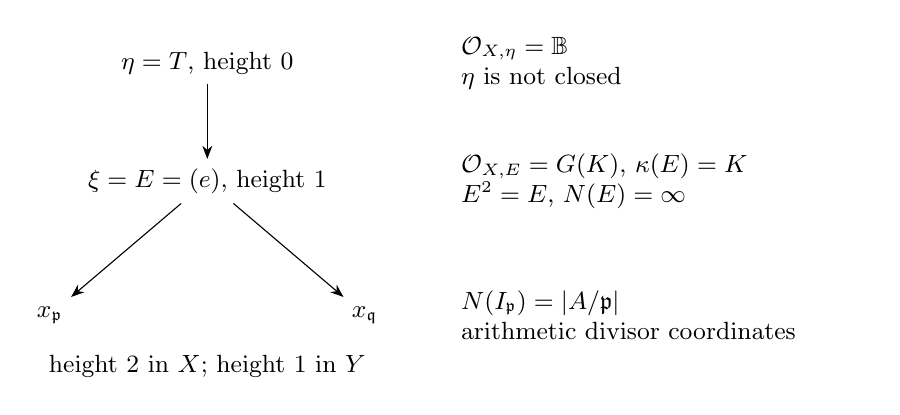
\begin{tikzpicture}[>=Stealth,every node/.style={font=\small}]
\node (eta) at (0,3.2) {\(\eta=T\), height \(0\)};
\node (e) at (0,1.7) {\(\xi=E=(e)\), height \(1\)};
\node (p) at (-2.0,0) {\(x_{\mathfrak p}\)};
\node (q) at (2.0,0) {\(x_{\mathfrak q}\)};
\draw[->] (eta)--(e);
\draw[->] (e)--(p);
\draw[->] (e)--(q);
\node at (0,-.65) {height \(2\) in \(X\); height \(1\) in \(Y\)};
\node[anchor=west,align=left,text width=5.1cm] at (3.1,3.2)
 {\(\mathcal O_{X,\eta}=\mathbb B\)\\\(\eta\) is not closed};
\node[anchor=west,align=left,text width=5.1cm] at (3.1,1.7)
 {\(\mathcal O_{X,E}=G(K)\), \(\kappa(E)=K\)\\\(E^2=E\), \(N(E)=\infty\)};
\node[anchor=west,align=left,text width=5.1cm] at (3.1,0)
 {\(N(I_{\mathfrak p})=|A/\mathfrak p|\)\\arithmetic divisor coordinates};
\end{tikzpicture}
\caption{Complete types of specialization in
\(X=\operatorname{Spec}G(\mathcal O_K)\). Arrows mean strict
inclusion of primes. The bottom points represent arbitrary distinct
finite primes, not a two-point spectrum.
Theorems~\ref{thm:sz-codimension} and \ref{thm:sz-norms} prove heights
and norms; Proposition~\ref{prop:sz-divisor-sequence} proves the
divisor map. The supported-zero prime is the prior result
\cite[\texttt{thm:zero-prime-not-irr}]{globalization}.}
\label{fig:sz-divisors}
\end{figure}

\subsection{Finite norms and the ideal zeta function}

\begin{theorem}[All integral ideal norms and closed points]\label{thm:sz-norms}
For an integral \(F\subseteq S\), let \(N_{\rm B}(F)\) be the
cardinality of its Bourne-congruence quotient. Then
\begin{equation}\label{eq:sz-all-norms}
 N_{\rm B}(T)=\infty,\qquad N_{\rm B}(E)=\infty,\qquad
 N_{\rm B}(I_J)=|A/J|\quad(0\ne J\subseteq A).
\end{equation}
The finite-norm ideals are exactly the regular integral ideals.
The closed points are exactly \(I_{\mathfrak p}\) for nonzero
primes \(\mathfrak p\), all with finite norm \(|A/\mathfrak p|\).
The point \(E\) is not closed in \(X\), has infinite quotient \(A\),
and infinite residue field \(K\). It is closed in its local spectrum
\(\operatorname{Spec}G(K)\), still with infinite residue field.
The generic point \(T\) has residue object \(\mathbb B\) of size
two, but is not closed and has infinite global ideal quotient.
\end{theorem}
\begin{proof}
The Bourne relation of \(T\) is equality, giving quotient \(S\).
The quotient calculation in Theorem~\ref{thm:sz-codimension}
gives \(S/E=A\) and \(S/I_J=A/J\). The first two quotients are
infinite, and nonzero ring ideals have finite quotient by
Lemma~\ref{lem:sz-dedekind}. Closed points are maximal primes,
as already classified. The spectrum of \(G(K)\) consists of
\(T\subsetneq E\), so \(E\) is closed there, with residue \(K\).
The remaining assertions follow from the stalk and closure table.
\end{proof}

\begin{proposition}[Norm homomorphism and Euler product]\label{prop:sz-zeta}
On regular fractional ideals the norm is
\[
 N(I_J)=\prod_{\mathfrak p}|A/\mathfrak p|^{v_{\mathfrak p}(J)}
 \in\mathbb Q_{>0}.
\]
It is multiplicative, with
\(N(cS)=|\operatorname{Norm}_{K/\mathbb Q}(c)|\) for \(c\in K^\times\).
The sum over all finite Bourne-norm ideals is
\begin{equation}\label{eq:sz-zeta}
 \zeta_{S,{\rm B}}(s)
 =\sum_{N_{\rm B}(F)<\infty}N_{\rm B}(F)^{-s}
 =\sum_{0\ne J\subseteq A}|A/J|^{-s}
 =\prod_{\mathfrak p\ne0}(1-|A/\mathfrak p|^{-s})^{-1}
 =\zeta_K(s)\quad(\operatorname{Re}s>1).
\end{equation}
Equation~\eqref{eq:sz-all-norms} accounts explicitly for both
zero ideals in this summation rule.
\end{proposition}
\begin{proof}
The ideal norm formula is Lemma~\ref{lem:sz-factorization}.
For \(0\ne c\in A\), multiplication by \(c\) on a \(\mathbb Z\)-basis
of \(A\) is a full-rank integer matrix with image \(cA\).
Its determinant's absolute value is the lattice index \([A:cA]\):
integer elementary operations put the matrix in Smith diagonal form,
where each quantity is the product of the positive diagonal entries.
The rational determinant is the field norm by definition.
For \(c=a/b\in K^\times\), multiplicativity gives the quotient
of these two identities.

Theorem~\ref{thm:sz-norms} proves the termwise equality of the sums.
Unique ideal factorization gives the Euler product as a sum of
nonnegative terms for real \(s>1\). To prove convergence, let
\(n=[K:\mathbb Q]\). Primes above a rational prime \(\ell\) have
residue sizes \(\ell^{f_{\mathfrak p}}\) with \(f_{\mathfrak p}\ge1\).
There are at most \(n\) such primes: the Chinese remainder surjection
\[
 A/\ell A\longrightarrow\prod_{\mathfrak p\mid\ell}A/\mathfrak p
\]
gives \(\sum_{\mathfrak p\mid\ell}f_{\mathfrak p}\le n\).
Every nonzero prime lies over a rational prime, since its residue
field is finite. Hence for real \(\sigma>1\),
\[
 \prod_{\mathfrak p}(1-|A/\mathfrak p|^{-\sigma})^{-1}
 \le\prod_{\ell\ {\rm prime}}(1-\ell^{-\sigma})^{-n}
 =\left(\sum_{m\ge1}m^{-\sigma}\right)^n<\infty.
\]
The last sum converges by the integral test; its product expression
follows from integer unique factorization and increasing finite
products. Thus all rearrangements are valid for complex \(s\)
with real part greater than one. The final ideal sum is the defining
Dedekind zeta series, proving \eqref{eq:sz-zeta}.
\end{proof}

The quotient retaining a separate absent element has its own exact
comparison map. For \(0\ne J\subseteq A\), set
\[
 x\equiv_J^{\rm sp}y
 \iff (x=y=\tau)\ \text{or}\ (x,y\in A,\ x-y\in J).
\]
Its quotient is \(G(A/J)\), of size \(|A/J|+1\), with zero class
\(T\), rather than \(I_J\). The natural morphism
\[
 G(A/J)\longrightarrow A/J,\qquad
 \tau\mapsto0,\quad[a]\mapsto[a],
\]
identifies exactly its two zero-amplitude elements and has kernel
\(\{\tau,0_{A/J}\}\). This proves the exact relation between the
two quotient constructions. Their weights obey
\[
 (N(J)+1)(N(H)+1)-(N(JH)+1)=N(J)+N(H).
\]
The support-preserving cardinality therefore has its stated counting
rule, while the Bourne norm retains the multiplicative formula
\eqref{eq:sz-zeta}.

% END COMPLETE PROOF SOURCE: divisor_derivation/06_divisors_and_norms.tex


% BEGIN COMPLETE PROOF SOURCE: 10_adelic_valuation_bridge.tex
\section{The full adelic valuation space and its derived geometry}


\subsection{Objects and source scope}

Throughout, a ring is commutative and has an identity. For a nonzero ring
$A$, define the semiring
\[
 \G(A)=\{\tau\}\sqcup A.
\]
The symbol $\tau$ is the additive identity and multiplicative absorber.
Addition and multiplication of two supported elements of $A$ are their
original ring operations, with their results remaining in the supported
copy of $A$. We write $e_A$ for its element $0_A$. Thus
\[
 \tau\ne e_A,\quad e_A+e_A=e_A,\quad
 a+(-a)=e_A,\quad e_Aa=e_A\quad(a\in A).
 \tag{AV1.1}\label{eq:split-identities}
\]
The last formula does not apply to $a=\tau$: $e_A\tau=\tau$.
All semiring homomorphisms below preserve the additive identity and the
multiplicative identity. Associativity and commutativity follow on supported
inputs from those of $A$ and otherwise from the rules for $\tau$.
Distributivity follows from that of $A$ when all three inputs are supported;
if the multiplier is $\tau$, both sides are $\tau$; if either summand is
$\tau$, the identity reduces to $a b=a b+\tau$. These checks prove that
$\G(A)$ is a semiring. A ring homomorphism $f:A\to B$ gives a semiring
homomorphism $\G(f)$ by $\tau\mapsto\tau$ and $a\mapsto f(a)$, including
$e_A\mapsto e_B$.

The human source used here is Antoine S\'edillot,
\emph{Topological adelic curves: Zariski-Riemann spaces, algebraic coverings,
Harder-Narsimhan filtrations and heights},
\href{https://arxiv.org/abs/2503.20156v2}{arXiv:2503.20156v2}.
The exact author file is \nolinkurl{topological_adelic_curves_V2.tex}.
Its definition of pseudo-absolute values is at source lines 623--629;
integral structures at lines 674--689, label
\nolinkurl{subsub:prelim_integral_structures}; the algebraic
Zariski--Riemann construction at lines 819--848, labels
\nolinkurl{subsub:Zariski-Riemann_space_algebraic} and
\nolinkurl{example:ZR_algebraic}; the general coherence and Tor assertion
at lines 942--985, label
\nolinkurl{prop:coherence_algeabraic_ZR_sheaf}.
The spelling of the latter label is retained so the locator matches the
source. The statements about split objects below are proved here. The
general Tor assertion of the source is examined in Section~\ref{sec:repair};
it is not used as a substitute for the proofs in this note.

\subsection{The entire space of split pseudo-absolute values}

Equip $[0,\infty]$ with its compact order topology. Extended addition has
$r+\infty=\infty$. Extended multiplication is used only away from the two
ordered pairs $(0,\infty)$ and $(\infty,0)$.

\begin{definition}
For a field $K$, let $\mathcal P(\G(K))$ consist of maps
$w:\G(K)\to[0,\infty]$ such that
\[
 w(\tau)=0,\qquad w(1)=1,\qquad
 w(a+b)\le w(a)+w(b),
 \tag{AV2.1}\label{eq:split-pav}
\]
and
\[
 w(ab)=w(a)w(b)\quad\hbox{if }
 \{w(a),w(b)\}\ne\{0,\infty\}.
 \tag{AV2.2}\label{eq:partial-mult}
\]
Give this set its topology of pointwise convergence. Let $M_K$ be the
space of pseudo-absolute values in S\'edillot's definition: the same
conditions on $K$, with $v(0_K)=0$ and $v(1)=1$.
\end{definition}

\begin{theorem}[Exact component decomposition]\label{thm:decomposition}
Define
\[
 \chi_K(\tau)=0,\qquad \chi_K(a)=1\ (a\in K),
 \qquad
 j_K(v)(\tau)=0,\quad j_K(v)(a)=v(a)\ (a\in K).
\]
Then
\[
 \mathcal P(\G(K))=\{\chi_K\}\sqcup j_K(M_K)
 \tag{AV2.3}\label{eq:components}
\]
is a homeomorphism of a disjoint union of two compact Hausdorff spaces.
The two components are respectively $w(e_K)=1$ and $w(e_K)=0$ and are
both open and closed. In particular, the full space is not identified
with $M_K$ by restriction to the supported coefficients.
\end{theorem}
\begin{proof}
Since $(-1)^2=1$, multiplicativity applies to the repeated value
$w(-1)$ and gives $w(-1)^2=1$. Neither zero nor infinity has square one,
so $w(-1)=1$. The equality $1+(-1)=e_K$ implies $w(e_K)\le2$.
The equality $e_K^2=e_K$ then gives $w(e_K)^2=w(e_K)$, whence
$w(e_K)\in\{0,1\}$.

If $w(e_K)=1$, then for every supported $a$ the pair
$(w(e_K),w(a))$ is allowed in \eqref{eq:partial-mult}; hence
$1=w(e_Ka)=w(a)$. Thus $w=\chi_K$. This map satisfies the triangle
inequality: the sum of two supported elements is supported, so its
value one is at most two; a sum involving $\tau$ is immediate.
It is multiplicative because a product is supported exactly when both
factors are supported.

If $w(e_K)=0$, its restriction to $K$ satisfies precisely S\'edillot's
three axioms. Conversely, any such $v$ extends by $v(\tau)=0$:
the new triangle inequalities are equalities and each newly required
product identity has value zero on both sides. This proves the bijection.
Both restriction and extension are continuous in the product topologies.
The continuous evaluation at $e_K$ takes only the values zero and one,
which have disjoint open neighbourhoods. It therefore makes both
components open and closed.

For completeness, $M_K$ is a closed subset of $[0,\infty]^K$.
The two value constraints and every triangle inequality are closed
conditions. For a convergent net satisfying multiplicativity, if its
limiting pair is allowed, it has a neighbourhood avoiding the two
forbidden pairs; extended multiplication is continuous at that pair,
so the limiting identity holds. Thus its multiplicativity condition
is closed as well. The product is compact Hausdorff and the trivial
absolute value supplies a point. This proves the compactness and
Hausdorff assertions, and then those of \eqref{eq:components}.
\end{proof}

\begin{proposition}[Field maps preserve both components]\label{prop:fieldfunctor}
A field embedding $i:K\hookrightarrow L$ induces a continuous restriction
$\mathcal P(\G(L))\to\mathcal P(\G(K))$. It sends $\chi_L$ to $\chi_K$
and $j_L(v)$ to $j_K(v|_K)$. Every extension of $\chi_K$ is $\chi_L$;
extensions of $j_K(v)$ correspond exactly to extensions of $v$ to $L$.
\end{proposition}
\begin{proof}
Precomposition preserves every displayed axiom and is continuous in
the pointwise topology. It preserves $e$, so preserves its value zero
or one. Theorem~\ref{thm:decomposition} then gives all assertions.
\end{proof}

\subsection{Finiteness, residue, and the complete prime space}

\begin{proposition}[Finiteness and residue proved from the axioms]
\label{prop:finite}
For $v\in M_K$ put
\[
 A_v=\{a\in K:v(a)<\infty\},\quad
 \mathfrak m_v=\{a\in K:v(a)=0\},\quad
 \kappa_v=A_v/\mathfrak m_v.
\]
Then $A_v$ is a valuation ring of $K$, its unique maximal ideal is
$\mathfrak m_v$, and $v$ induces an absolute value $\overline v$ on
$\kappa_v$. The finite locus of $j_K(v)$ is exactly $\G(A_v)$.
\end{proposition}
\begin{proof}
As above, $v(-1)=1$, so $v(-a)=v(a)$. The triangle and product axioms
make $A_v$ a subring and $\mathfrak m_v$ an ideal in $A_v$.
For $a\ne0$, the identity $aa^{-1}=1$ gives the following exhaustive
possibilities. If $0<v(a)<\infty$, then $v(a^{-1})=v(a)^{-1}$:
all pairs with the positive finite value $v(a)$ are allowed. If $v(a)=0$,
then $v(a^{-1})$ must be infinity, since every finite alternative would
give product value zero. If $v(a)=\infty$, then $v(a^{-1})$ must be zero,
since every nonzero alternative would give product value infinity.
Consequently $a$ or $a^{-1}$ belongs to $A_v$, proving the valuation
property, and its units are precisely the elements of positive finite
value. This proves the assertion about the maximal ideal.

If $a-b\in\mathfrak m_v$, the triangle inequality gives $v(a)\le v(b)$
and $v(b)\le v(a)$; hence the value depends only on the residue class.
It vanishes precisely on the zero class, is finite there, and satisfies
the ordinary triangle and multiplication laws. Thus it is an absolute
value of the residue field. The final assertion follows from the value
zero of $\tau$.
\end{proof}

\begin{proposition}[All ideals and all primes]\label{prop:ideals}
For every nonzero ring $A$, the ideals of $\G(A)$ are $\{\tau\}$ and
\[
 I^+=\{\tau\}\sqcup I\qquad(I\text{ an ideal of }A).
 \tag{AV3.1}\label{eq:liftideal}
\]
Its proper prime ideals are $\{\tau\}$ and $\mathfrak p^+$ for
$\mathfrak p\in\Spec A$. The map
$\mathfrak p\mapsto\mathfrak p^+$ identifies $\Spec A$ with the closed
subset $V(e_A)$ of $\Spec\G(A)$. The remaining point $\{\tau\}$ is open
and is a generalization of every point. For supported $a$,
\[
 D_{\G(A)}(a)=\{\{\tau\}\}\sqcup D_A(a),\qquad
 D_{\G(A)}(e_A)=\{\{\tau\}\}.
 \tag{AV3.2}\label{eq:opens}
\]
If $A$ is a domain and $\mathfrak p$ a nonzero prime, its original chain
is retained as
\[
 (\tau)=\{\tau\}\ \subsetneq\ (e_A)=\{\tau,e_A\}
 \ \subsetneq\ \mathfrak p^+.
 \tag{AV3.3}\label{eq:chain}
\]
\end{proposition}
\begin{proof}
An ideal containing a supported element contains $e_A$ by multiplication
by $e_A$. Its supported elements are closed under addition, multiplication
by every element of $A$, and negatives by multiplication by $-1$; hence
they form a ring ideal. The converse follows directly from the operations.
A product of two supported elements is always supported, even when its
coefficient is zero, proving primality of $\{\tau\}$. Primality of
$\mathfrak p^+$ is exactly primality of $\mathfrak p$ in $A$.
The formulas for the basic opens follow by membership in these ideals;
they prove the topological assertions and the strict chain.
\end{proof}

\begin{theorem}[Residue map with supported zero]\label{thm:residue}
For $v\in M_K$ there is a commuting diagram of semirings
\[
\begin{tikzcd}[column sep=large,row sep=large]
 \G(A_v) \arrow[r,"\G(\pi_v)"] \arrow[d,"q_{A_v}"'] &
 \G(\kappa_v) \arrow[d,"q_{\kappa_v}"]\\
 A_v \arrow[r,"\pi_v"'] & \kappa_v .
\end{tikzcd}
\tag{AV3.4}\label{eq:residue-square}
\]
Here $q_A(\tau)=q_A(e_A)=0_A$ and $q_A(a)=a$ on supported coefficients.
The top map is surjective and local: its inverse image of the unique
maximal ideal $\{\tau,e_{\kappa_v}\}$ is
$\mathfrak m_v^+$. Its fibre over the additive identity is only $\{\tau\}$.
Its full congruence is
\[
 \tau\sim\tau,\qquad
 a\sim b\ \Longleftrightarrow\ a-b\in\mathfrak m_v
 \quad(a,b\in A_v),
 \tag{AV3.5}\label{eq:residue-congruence}
\]
with no equivalence of $\tau$ and a supported element.
On $\G(A_v)$ one has
\[
 j_K(v)=j_{\kappa_v}(\overline v)\circ\G(\pi_v).
 \tag{AV3.6}\label{eq:residue-value-factor}
\]
\end{theorem}
\begin{proof}
Every map in \eqref{eq:residue-square} respects its stated operations;
on a supported input both composites are its residue coefficient and
on $\tau$ both are zero. The assertions concerning fibres, congruence,
and localness follow respectively from preservation of support, equality
of residue coefficients, and Proposition~\ref{prop:ideals}.
The last formula is Proposition~\ref{prop:finite} on supported elements
and the value zero on $\tau$.
\end{proof}

The restriction to the finite locus is essential. If $0\ne a\in
\mathfrak m_v$, then $v(a)=0$, $v(a^{-1})=\infty$, and $v(aa^{-1})=1$.
Thus $\{w=0\}$ is generally not an ideal of $\G(K)$; it becomes the
prime ideal $\mathfrak m_v^+$ of $\G(A_v)$. The precise defect is the set
of forbidden products
\[
 \mathcal D_v=\{(a,b)\in K^2:v(a)=0,\ v(b)=\infty\}
 \cup\{(a,b):v(a)=\infty,\ v(b)=0\}.
\]
The restriction map to $\G(A_v)$ removes every such pair and gives the
exact residue factorization \eqref{eq:residue-value-factor}; it does not
identify the two zeros.

\subsection{Integral structures and the support point}

Let $A$ be a Pr\"ufer domain with fraction field $K$. Here this means that
every $A_{\mathfrak p}$ is a valuation ring. Let $\|\cdot\|$ be a Banach
ring norm as in S\'edillot's integral-structure definition. A bounded
multiplicative seminorm $\alpha$ on $A$ means a finite map to
$[0,\infty)$ with $\alpha(0)=0$, $\alpha(1)=1$, triangle inequality,
multiplicativity, and $\alpha(a)\le\|a\|$.

\begin{proposition}[Exact extension from the integral spectrum]
\label{prop:integral}
Restriction is a bijection between such $\alpha$ and the subset
\[
 M_{K,A}=\{v\in M_K:v(a)\le\|a\|\text{ for all }a\in A\}.
 \tag{AV4.1}\label{eq:integral-subspace}
\]
For $\mathfrak p=\ker\alpha$, the inverse map has finiteness ring
$A_{\mathfrak p}$ and is given by
\[
 v_\alpha(x)=
 \begin{cases}
  \overline\alpha(x\bmod\mathfrak p A_{\mathfrak p}),&x\in A_{\mathfrak p},\\
  \infty,&x\notin A_{\mathfrak p},
 \end{cases}
 \tag{AV4.2}\label{eq:extension}
\]
where $\overline\alpha$ is the absolute value on
$\kappa(\mathfrak p)=\Frac(A/\mathfrak p)$ defined by
$\overline\alpha(\overline a/\overline b)=\alpha(a)/\alpha(b)$.
The subset \eqref{eq:integral-subspace} is closed in $M_K$, and this
bijection is a homeomorphism for the pointwise topologies.
\end{proposition}
\begin{proof}
Multiplicativity makes $\mathfrak p$ prime. The triangle inequality proves
that $\alpha$ depends only on a residue class, as in
Proposition~\ref{prop:finite}, and its quotient norm extends uniquely by
the indicated fraction formula. The residue field of $A_{\mathfrak p}$
is exactly $\Frac(A/\mathfrak p)$ because its nonzero residue denominators
are the elements outside $\mathfrak p$.

For any valuation ring $V\subset K$ with maximal ideal $\mathfrak m$
and residue absolute value $\beta$, the map equal to $\beta$ on residues
of $V$ and infinity outside $V$ satisfies the pseudo-absolute-value
axioms. To verify this, sums of two finite inputs use the residue triangle
inequality and other sums have infinite right side. Products of finite
inputs use the residue multiplication law. An element outside $V$ has
inverse in $\mathfrak m$. Multiplication by a unit of $V$ preserves its
being outside $V$, and the product of two outside elements is outside
because its inverse is a product in $\mathfrak m$. The sole remaining
case is one residue-zero factor and one infinite factor, for which no
identity is imposed. This proves existence of \eqref{eq:extension}.

For uniqueness let $v$ restrict to $\alpha$. Since every element of $A$
is finite, $A\subset A_v$. All elements of $A\setminus\mathfrak p$ are
units of $A_v$, giving $A_{\mathfrak p}\subset A_v$ with the displayed
residue values. If $x\in A_v\setminus A_{\mathfrak p}$, the valuation
property implies $x^{-1}\in\mathfrak p A_{\mathfrak p}$, whose value is
zero. But then multiplicativity for the finite pair $(x,x^{-1})$ would
give $v(1)=0$, a contradiction. Thus the finiteness ring and every value
are forced.

Each inequality in \eqref{eq:integral-subspace} is closed in the pointwise
topology. This subset is compact by Theorem~\ref{thm:decomposition}.
Restriction is a continuous bijection into a Hausdorff product space,
so its inverse is continuous: a closed subset of a compact domain has
compact, hence closed, image in a Hausdorff space.
\end{proof}

\begin{corollary}[What a bound does to the split point]
Extend the norm bound by $\|\tau\|=0$ and
$\|e_A\|=\|0_A\|=0$. The maps in $\mathcal P(\G(K))$ obeying this bound
on $\G(A)$ are precisely $j_K(M_{K,A})$. In particular $\chi_K$ does not
obey it. The full split extension of the integral space is instead the
explicit disjoint union $\{\chi_K\}\sqcup j_K(M_{K,A})$.
\end{corollary}
\begin{proof}
The character has $\chi_K(e_A)=1>0$, whereas every lifted valuation has
value zero there. On every other supported input the bound is exactly
\eqref{eq:integral-subspace}. Apply Theorem~\ref{thm:decomposition}.
\end{proof}

\begin{proposition}[The center map includes the additional prime]
\label{prop:centermap}
For the explicit space
$\widetilde M_{K,A}=\{\chi_K\}\sqcup j_K(M_{K,A})$, there is a
continuous map
\[
 c_A:\widetilde M_{K,A}\longrightarrow\Spec\G(A),\qquad
 c_A(\chi_K)=\{\tau\},\qquad
 c_A(j_K(v))=(\mathfrak m_v\cap A)^+.
 \tag{AV4.3}\label{eq:center-map}
\]
At $j_K(v)$, writing $\mathfrak p=\mathfrak m_v\cap A$, the associated
local semiring is $\G(A)_{\mathfrak p^+}=\G(A_{\mathfrak p})=\G(A_v)$.
At the additional prime one instead has
$\G(A)_{\{\tau\}}\cong\mathbb B$, where
$\mathbb B=\{0,1\}$ has $1+1=1$.
\end{proposition}
\begin{proof}
The values of $v$ are finite on $A$, so its zero locus there is a prime
ideal, by multiplication of finite nonnegative values. For a supported
$a\in A$, the inverse image of the basic open $D(a)$ is
$\{\chi_K\}\sqcup\{j_K(v):v(a)>0\}$, which is open in the stated
pointwise topology. The inverse image of $D(\tau)$ is empty. These
opens prove continuity.

For the local semiring at $\mathfrak p^+$, denominators are exactly
supported $s\in A\setminus\mathfrak p$. Send a supported fraction
$a/s$ to its supported coefficient in $A_{\mathfrak p}$ and the
fraction $\tau/s$ to $\tau$. The usual cross-multiplication criterion
proves equality of two supported fractions exactly when their ring
fractions agree; no supported fraction equals a $\tau$ fraction since
multiplication of supported elements stays supported. This proves the
first localization isomorphism. The equality with $A_v$ was proved in
Proposition~\ref{prop:integral}.

At $\{\tau\}$ every supported element, including $e_A$, is inverted.
An invertible multiplicative idempotent equals one, so $e_A=1$ in that
localization. Then $e_Aa=e_A$ forces every supported $a$ to equal one.
The two classes remain distinct because the support map to $\mathbb B$
sends all supported denominators to a unit, and therefore factors
through the localization while distinguishing their class from $\tau$.
Its addition is $1+1=1$ by the image of $e_A+e_A=e_A$.
\end{proof}

\subsection{The exact additive bridge and its limits}

\begin{theorem}[Universal ring recovery]\label{thm:ring-recovery}
The map $q_A:\G(A)\to A$ is universal among semiring homomorphisms from
$\G(A)$ to rings. It identifies exactly $\tau$ and $e_A$ and keeps all
other coefficients distinct. Consequently the category of
$\G(A)$-semimodules whose additive monoid is an abelian group is
canonically equivalent to the category of $A$-modules, by restriction
along $q_A$. Under this equivalence tensor products, resolutions, and
$\Tor$ are exactly the ordinary $A$-module constructions.
\end{theorem}
\begin{proof}
If $f:\G(A)\to R$ is a semiring homomorphism with $R$ a ring, then
$f(e_A)+f(e_A)=f(e_A)$ implies $f(e_A)=0$. It already sends $\tau$ to
zero. Its restriction to supported $A$ preserves addition,
multiplication, and identities, hence is a ring homomorphism. It is
uniquely determined and factors $f$ through $q_A$.

On an abelian-group semimodule $M$, the relation
$e_Am+e_Am=e_Am$ similarly gives $e_Am=0_M$ for all $m$. The action
therefore factors through $A$, and all semimodule homomorphisms are
precisely $A$-linear maps. Conversely every $A$-module gives such an
action. These are inverse functors and preserve each addition and
scalar action. A balanced biadditive map for one description is exactly
one for the other, so the tensor universal properties agree. Free and
projective objects, exact sequences, and tensor resolutions in this
abelian category therefore agree, proving the Tor assertion.
\end{proof}

There is also a way to retain the two zeros on modules. For an $A$-module
$M$, put $\G(M)=\{\tau_M\}\sqcup M$, with supported addition inherited
from $M$, and the scalar action induced from $A$, with either $\tau$
input absorbing. The semimodule laws follow by the same cases as in
\eqref{eq:split-identities}.

\begin{proposition}[Support-preserving module category]
\label{prop:module-support}
A homomorphism $h:\G(M)\to\G(N)$ is either the constant map to
$\tau_N$, or is $\G(f)$ for a unique $A$-linear map $f:M\to N$.
The morphisms preserving supported elements form a category equivalent
to $A$-modules. Its additive zero morphism is the supported map
$m\mapsto0_N$, extended by $\tau_M\mapsto\tau_N$; it differs from the
constant-$\tau_N$ homomorphism in the ambient semimodule category.
For every linear $f$,
\[
 (\G(f))^{-1}(\{\tau_N\})=\{\tau_M\},\qquad
 \G(\ker f)=\{\tau_M\}\sqcup\{m:f(m)=0_N\}.
 \tag{AV5.1}\label{eq:module-kernels}
\]
The second expression, with its inclusion, is the kernel in the
support-preserving category; the first is the categorical zero fibre
in the ambient category.
\end{proposition}
\begin{proof}
The only additive idempotents in $\G(N)$ are $\tau_N$ and $0_N$:
a supported idempotent satisfies $n+n=n$ in a group, so $n=0_N$.
Hence $h(0_M)$ is one of these. If $h(0_M)=\tau_N$, then
$h(m)+h(-m)=\tau_N$ forces both summands to be $\tau_N$, since any
supported summand makes a sum supported. This is the constant map.
If $h(0_M)=0_N$, the identity $0_M+m=m$ rules out $h(m)=\tau_N$,
because $0_N+\tau_N=0_N\ne\tau_N$. Thus all supported elements have
supported images. The homomorphism laws become exactly linearity of
$f=h|_M$. Conversely every linear map extends, proving the categorical
claim. The two kernel statements now follow by direct inverse-image
calculation, including the distinct images of $0_M$ and $\tau_M$.
\end{proof}

In particular, no assertion about derived functors in the entire
nonadditive semimodule category follows merely by renaming ordinary
module Tor. Theorem~\ref{thm:ring-recovery} and
Proposition~\ref{prop:module-support} specify two exact functors and
the exact categories in which the asserted transfer holds.

\subsection{Valuation stalks and the sheaf that retains support}

\begin{proposition}[Tor bound over a valuation ring]
\label{prop:valuation-tor}
Let $V$ be a valuation ring with fraction field $F$. Every torsion-free
$V$-module is flat. Every $V$-module has a flat resolution of length at
most one. Every finitely presented $V$-module has a finite free
resolution of length at most one. Consequently
\[
 \Tor_i^V(M,N)=0\qquad(i\ge2)
 \tag{AV6.1}\label{eq:torvanishing}
\]
for all $V$-modules $M,N$.
\end{proposition}
\begin{proof}
First a finitely generated torsion-free module is free. Given generators
$m_1,\ldots,m_n$, if they are dependent choose a nonzero relation
$\sum a_i m_i=0$. Among its nonzero coefficients choose $a_j$ dividing
all the others; this is possible because principal ideals in a valuation
ring are totally ordered. Write $a_i=a_jb_i$, with $b_j=1$.
Torsion-freeness gives $\sum b_i m_i=0$, expressing $m_j$ in the other
generators. Repeating decreases the number of generators until an
independent generating set remains. This is a free basis.

An arbitrary torsion-free module is the filtered union of its finitely
generated submodules, all free by the preceding argument. It is flat:
tensor commutes with filtered colimits, and filtered colimits preserve
injections and exactness of modules. Explicitly, a finite tensor relation
already lies in some finitely generated submodule, and if its image
vanishes in the colimit it vanishes at a later stage; exactness there
gives exactness in the colimit. Thus no relation obstructing flatness
appears in the union.

Choose a free surjection $P\twoheadrightarrow M$. Its kernel is a
submodule of a free module over a domain and so is torsion-free, hence
flat. This is the claimed length-one flat resolution. If $M$ is finitely
presented, choose $P$ finite free and its kernel finitely generated;
that kernel is then finite free by the first paragraph. Tensoring either
resolution proves \eqref{eq:torvanishing}.
\end{proof}

If $(Z,\mathcal O_Z)$ is a locally ringed space with valuation-ring
stalks, then for all sheaves of modules $\mathcal F,\mathcal H$,
\[
 \mathcal{T}or_i^{\mathcal O_Z}(\mathcal F,\mathcal H)=0\quad(i\ge2).
 \tag{AV6.2}\label{eq:sheaf-tor}
\]
Indeed stalks commute with tensor and homology; applying a flat resolution
and taking stalks identifies the stalk of this sheaf with
$\Tor_i^{\mathcal O_{Z,z}}(\mathcal F_z,\mathcal H_z)$, which vanishes
by Proposition~\ref{prop:valuation-tor}. A sheaf with all stalks zero is
zero, since every section whose germs vanish vanishes on a neighbourhood
of each point and hence globally by the sheaf axiom.

There is a small sheaf issue that matters for retaining support.
The assignment $U\mapsto\G(\mathcal O_Z(U))$ need not itself be a sheaf:
on two disjoint nonempty opens, a supported section on one and $\tau$ on
the other must be able to glue. Define instead
\[
 \mathcal S_Z(U)=\{(C,s):C\subset U\text{ is open and closed},\quad
                         s\in\mathcal O_Z(C)\}.
 \tag{AV6.3}\label{eq:split-sheaf}
\]
For $C=\varnothing$ the unique pair is $\tau$. Addition has support
$C\cup D$ and is the original sum on $C\cap D$, the first section on
$C\setminus D$, and the second on $D\setminus C$. Multiplication has
support $C\cap D$ and is the original product there. These pieces are
open and closed in the union, so the sheaf axiom for $\mathcal O_Z$
defines each operation. In particular cancellation on $C\cap D$ leaves
a supported zero.

\begin{proposition}[Sheaf-level split and recovery]
\label{prop:sheafsplit}
The construction \eqref{eq:split-sheaf} is a sheaf of semirings with
stalk $\mathcal S_{Z,z}=\G(\mathcal O_{Z,z})$. Extension by zero on
$U\setminus C$ gives a morphism $q:\mathcal S_Z\to\mathcal O_Z$ which
has the universal ring-recovery property stalkwise and as a sheaf.
Sheaves of $\mathcal S_Z$-semimodules with abelian-group addition are
exactly sheaves of $\mathcal O_Z$-modules. If the stalks of
$\mathcal O_Z$ are valuation rings, their Tor sheaves in this abelian
category obey \eqref{eq:sheaf-tor}.
\end{proposition}
\begin{proof}
Compatible supports on an open cover glue to a subset whose membership
is locally constant, hence to an open-and-closed subset. The supported
sections then glue uniquely by the original sheaf axiom. All semiring
identities hold locally according to whether each support is present,
and there reduce to the verified identities of $\G$.
A germ either has absent support on a neighbourhood or has full support
on a neighbourhood. These alternatives give respectively $\tau$ and
a unique supported coefficient germ, proving the stalk identification.
The extension-by-zero map is compatible with restrictions and
operations by the same local cases. Any map to a sheaf of rings factors
uniquely on stalks by Theorem~\ref{thm:ring-recovery}; equivalently, a
local section splits on its support and its complement, where the
factorizations are unique and so glue. The action on every additive-group
semimodule likewise factors locally and uniquely, giving the stated
equivalence. Its tensor products agree on stalks by
Theorem~\ref{thm:ring-recovery}, and hence as sheaves; the Tor conclusion
follows from \eqref{eq:sheaf-tor}.
\end{proof}

\subsubsection{The full spectral extension, including the extra generic point}

Let $(Z,\mathcal O_Z)$ be a nonempty irreducible locally ringed space
whose local rings are nonzero. Form the space
\[
 Z^+=Z\sqcup\{\eta_\tau\}
 \tag{AV6.4}\label{eq:full-spectrum-space}
\]
whose opens are the empty set, $\{\eta_\tau\}$, and
$U_W=\{\eta_\tau\}\cup W$ for nonempty open $W\subset Z$.
These sets form a topology: arbitrary unions are of the same form,
and a finite intersection is obtained by intersecting the corresponding
opens in $Z$, with empty intersection there giving $\{\eta_\tau\}$.
Define
\[
 \mathcal O_Z^+(U_W)=\G(\mathcal O_Z(W)),\qquad
 \mathcal O_Z^+(\{\eta_\tau\})=\mathbb B.
 \tag{AV6.5}\label{eq:full-spectrum-sheaf}
\]
Restriction between two opens with nonempty arithmetic parts is the
split extension of the original restriction map. Restriction to
$\{\eta_\tau\}$ sends $\tau$ to $0$ and every supported section to $1$.
This is a semiring homomorphism to $\mathbb B$: supported sums and
products remain supported, including supported zero coefficients.
On the empty open take the one-element semiring. The restriction maps
compose because ordinary restriction never changes the support tag.

\begin{theorem}[Full spectral gluing and stalks]\label{thm:fullspectral}
The construction \eqref{eq:full-spectrum-sheaf} is a sheaf of local
semirings. Its stalks are
\[
 \mathcal O_{Z,\eta_\tau}^+=\mathbb B,\qquad
 \mathcal O_{Z,z}^+=\G(\mathcal O_{Z,z})\quad(z\in Z).
 \tag{AV6.6}\label{eq:full-spectrum-stalks}
\]
The inclusion $i:Z\hookrightarrow Z^+$ is a closed embedding of spaces.
The inverse-image sheaf $i^{-1}\mathcal O_Z^+$ is the split sheaf
$\mathcal S_Z$ of Proposition~\ref{prop:sheafsplit}; its universal
ring quotient is $\mathcal O_Z$.
If $Z=\Spec A$ for a domain $A$, this construction is canonically the
entire semiring spectrum $\Spec\G(A)$ with its localization sheaf,
not only its closed arithmetic subset.
\end{theorem}
\begin{proof}
Every nonempty open of $Z^+$ contains $\eta_\tau$. On any cover of such
an open, compatible sections must therefore have the same image in
the stalk $\mathbb B$ at $\eta_\tau$. If that image is zero, each section
on an open with arithmetic part is $\tau$, and every section on the
singleton is zero; they glue uniquely to the absent section. If that
image is one, the sections on the arithmetic parts are supported.
Their coefficients agree wherever the arithmetic parts overlap,
because supported equality in $\G$ is coefficient equality. The
original sheaf axiom glues these coefficients to one section on $W$,
giving the unique supported glue on $U_W$. Sections on a singleton
member of the cover must be one and impose exactly that support
condition. This also proves the sheaf axiom for a cover of the
singleton. In the irreducible case, nonempty arithmetic opens intersect,
so the coefficient compatibility can equivalently be checked directly
on their nonempty intersections.

The singleton is a smallest neighbourhood of $\eta_\tau$, yielding
its stalk. Neighbourhoods of an arithmetic point $z$ are exactly $U_W$
for neighbourhoods $W$ of $z$. In their colimit no restriction identifies
$\tau$ with a supported section, and supported germs are precisely
$\mathcal O_{Z,z}$. This proves \eqref{eq:full-spectrum-stalks}.
If $(R,\mathfrak m)$ is a local ring, Proposition~\ref{prop:ideals}
shows that $\G(R)$ has the unique maximal ideal $\mathfrak m^+$.
The Boolean stalk has the unique maximal ideal $\{0\}$.
Thus all stalks are local semirings.

The complement of $i(Z)$ is the open singleton. Its relative topology
is the original topology of $Z$. The presheaf computing the inverse
image of $\mathcal O_Z^+$ on an open $W\subset Z$ has the restriction
of $\G(\mathcal O_Z(W))$ as a cofinal representative, because $U_W$
is the smallest open of $Z^+$ containing $i(W)$. Sheafifying this
presheaf allows the support tag to vary locally, giving exactly the
open-and-closed supported subsets and coefficient sections of
\eqref{eq:split-sheaf}. The construction in
Proposition~\ref{prop:sheafsplit} proves the ring quotient assertion.

For a domain $A$, Proposition~\ref{prop:ideals} identifies the points
and opens with $Z^+$, taking $\eta_\tau$ to the prime $\{\tau\}$.
For a nonzero supported $a$, the basic open $D_{\G(A)}(a)$ has
arithmetic part $D_A(a)$, and its local-fraction semiring is
$\G(A)_a\cong\G(A_a)$, by the same cross-multiplication calculation
as Proposition~\ref{prop:centermap}. This agrees with
$\G(\mathcal O_Z(D_A(a)))$. The remaining nonempty basic open
$D_{\G(A)}(e_A)=\{\eta_\tau\}$ has localization $\mathbb B$ by that
proposition. All restriction maps agree: between arithmetic charts
they are localization maps, and to the singleton they retain exactly
the support. Since these form a basis, gluing identifies their
localization sheaf with \eqref{eq:full-spectrum-sheaf}.
\end{proof}

\begin{proposition}[Every local morphism extends with its support point]
\label{prop:fullspectralfunctor}
Let $f:(Z,\mathcal O_Z)\to(X,\mathcal O_X)$ be a morphism of nonempty
irreducible locally ringed spaces with nonzero local rings. Then
\[
 f^+:Z^+\longrightarrow X^+,\qquad
 f^+(z)=f(z),\quad f^+(\eta_{\tau,Z})=\eta_{\tau,X}
 \tag{AV6.7}\label{eq:full-morphism}
\]
is canonically a morphism of locally semiringed spaces. At an arithmetic
point its stalk map is $\G(f_z^\#)$, and at the extra point it is the
identity of $\mathbb B$. The construction respects identities and
composition, and its restriction followed by coefficient recovery
is the original morphism $f$.
\end{proposition}
\begin{proof}
The inverse image of $U_W$ is
$\{\eta_{\tau,Z}\}\cup f^{-1}(W)$, an open of $Z^+$ even when the
arithmetic inverse image is empty. If it is nonempty, use
$\G(f^\#):\G(\mathcal O_X(W))\to
\G(\mathcal O_Z(f^{-1}W))$ on sections. If it is empty, use the support
homomorphism to $\mathbb B$. On the singleton use its identity.
These homomorphisms respect restrictions, including restrictions that
make the arithmetic part empty, because coefficient maps preserve the
support tag. They therefore define a sheaf morphism and give the stated
stalk maps. A local ring map has inverse image of the maximal ideal
equal to the maximal ideal. Formula \eqref{eq:liftideal} shows the same
for its split extension. The Boolean identity is local as well.
Composition and recovery hold on every supported coefficient and on
$\tau$, proving every remaining assertion.
\end{proof}

\subsection{The exact scope of the Tor assertion and its refinement}
\label{sec:repair}

\subsubsection{The whole-scheme submodel limit does not have the claimed bound}

In the supplied source a projective submodel of a projective $K$-scheme
$X$ over $k\subset K$ is a factorization $X\to\mathcal X\to\Spec k$
with schematically dominant first map and projective second map.
Its Zariski--Riemann space is the inverse limit of these submodels.

\begin{proposition}[An explicit counterexample to the unrestricted claim]
\label{prop:source-counterexample}
If $k=K$ and $X$ is a projective $K$-scheme, this submodel limit is $X$.
For $X=\mathbf P^2_K$, a coherent point sheaf has nonzero $\Tor_2$ with
itself. Thus the source's assertion of Tor-dimension at most one for
all coherent sheaves on its general $\mathrm{ZR}(X/k)$, with only its
stated hypotheses, fails in this case.
\end{proposition}
\begin{proof}
The identity factorization makes $X$ itself a submodel, and the defining
map $X\to\mathcal X$ is the unique arrow from this object to each
submodel compatible with the factorization. For any compatible cone,
its map to the $X$ component determines every other component.
Therefore the inverse limit is $X$, also as a locally ringed space.

Take a $K$-rational point with affine coordinates $x=y=0$. Its local ring
is $R=K[x,y]_{(x,y)}$, with residue field $K$. The sequence
\[
 0\longrightarrow R\xrightarrow{c\mapsto(-yc,xc)}R^2
 \xrightarrow{(a,b)\mapsto xa+yb}R\longrightarrow K\longrightarrow0
 \tag{AV7.1}\label{eq:koszul}
\]
is exact. The left map is injective because $R$ is a domain. If
$xa+yb=0$, reduction modulo $x$ in the domain $K[y]_{(y)}$ gives
$b\equiv0\pmod x$, so $b=xc$, and then $a=-yc$. The image at $R$ is
the ideal $(x,y)$, giving the last exactness. Tensoring with $K$ makes
both differentials zero, so $\Tor_2^R(K,K)=K\ne0$.
The coherent skyscraper sheaf at the point therefore has a nonzero
second Tor stalk with itself. All the stated hypotheses hold: $K$ is
stably coherent, and $\mathbf P^2_K$ is projective and integral.
\end{proof}

\subsubsection{The valuation refinement is a new space with an exact map}

Let $X$ be an integral separated scheme of finite type over a field and
$F=K(X)$ its actual function field. Consider integral schemes $Y$ with
a projective birational morphism $Y\to X$, and compatible morphisms
over $X$. Their category is cofiltered: the closure of the common
generic point in $Y_1\times_XY_2$ is another such integral model
dominating both. Define
\[
 \mathfrak Z_X=\varprojlim_{Y\to X}Y,\qquad
 \mathcal O_{\mathfrak Z_X}
   =\varinjlim_{Y\to X}p_Y^{-1}\mathcal O_Y.
 \tag{AV7.2}\label{eq:valuation-refinement}
\]
The limit topology and the indicated sheaf are used. Stalks are the
filtered colimits of the local rings at compatible centers; these
colimits are local because all transition maps between these local
rings are local. The projection to the identity model is a morphism of
locally ringed spaces $\rho:\mathfrak Z_X\to X$.

\begin{theorem}[Valuation refinement and the proved amplitude bound]
\label{thm:valuationrefinement}
Points of $\mathfrak Z_X$ are in bijection with pairs $(V,c)$ where $V$
is a valuation ring of $F$ and $c:\Spec V\to X$ extends the generic
point $\Spec F\to X$. At the corresponding point $z$, the stalk is
exactly $V$. If $x=c(\mathfrak m_V)$, the stalk map of $\rho$ is the
inclusion $\mathcal O_{X,x}\hookrightarrow V$. All sheaves of modules
on $\mathfrak Z_X$ satisfy
\[
 \mathcal{T}or_i^{\mathcal O_{\mathfrak Z_X}}(\mathcal F,\mathcal H)=0
 \quad(i\ge2).
 \tag{AV7.3}\label{eq:refinement-tor}
\]
The split sheaf from \eqref{eq:split-sheaf} has stalks $\G(V)$ and
maps to this ringed space by the exact coefficient quotient; its
abelian-group module category has the same bound.
\end{theorem}
\begin{proof}
Given $(V,c)$ and a model $Y\to X$, its generic map lifts uniquely to
$\Spec V\to Y$. This is the valuative property of a projective map;
it can be checked here using homogeneous coordinates: write the
generic lift as $[a_0:\cdots:a_n]$ in a projective embedding of $Y$,
divide by an $a_j$ whose value is least among these finitely many
nonzero coordinates, and obtain coordinates in $V$ with one equal to
one. The homogeneous equations hold over $V$ because they hold over
$F$. Uniqueness follows from separatedness, since two maps agreeing
at the generic point agree on the closed equations of the diagonal.
These unique lifts give compatible centers $z_Y$ and therefore $z$.
Each local ring $\mathcal O_{Y,z_Y}$ embeds locally into $V$.

Conversely, a compatible family gives a union
$R_z=\varinjlim_Y\mathcal O_{Y,z_Y}\subset F$. For each $f\in F^*$,
take the closure of the graph of its rational map to $\mathbf P^1$
inside $X\times\mathbf P^1$. It is an integral projective birational
model. Its center lies in at least one of the two standard affine
charts, so either $f$ or $f^{-1}$ belongs to its local ring and hence
to $R_z$. Therefore $R_z$ is a valuation ring. Each center map is local,
and the inclusion of the $X$ local ring gives the required center on $X$.

For the family constructed from $V$, the union of center rings equals
$V$, rather than just being contained in it. If $f\in V$, the graph
model just used has center in its finite-coordinate chart: its unique
$V$-lift has coordinate $f$, which is defined at the closed point of
$\Spec V$. Thus $f$ lies in that center's local ring. Every element
of $V$ is obtained. The construction is inverse in the other direction
because the inclusions of center rings into the union give the unique
lifts to each separated model. This proves both the bijection and the
stalk and morphism formulas. The Tor assertions follow from
\eqref{eq:sheaf-tor} and Proposition~\ref{prop:sheafsplit}.
\end{proof}

The distinction between \eqref{eq:valuation-refinement} and the source's
whole-scheme submodels is an explicit morphism $\rho$ and a change of
modification problem: the former models the generic map $\Spec F\to X$,
whereas the latter requires the whole map $X\to\mathcal X$ to survive.
For $X=\Spec K$ over a subring, valuation centers recover the valuation
stalk setting recalled in S\'edillot's
\nolinkurl{example:ZR_algebraic}, source lines 831--835. The bound is
therefore proved on the valuation objects needed by that field-level
route without asserting it on every whole-scheme submodel limit.

\begin{corollary}[The entire spectrum survives valuation refinement]
\label{cor:fullrefinement}
The space $\mathfrak Z_X$ in Theorem~\ref{thm:valuationrefinement} is
irreducible with generic point represented by the valuation ring $F$.
The refinement induces the exact morphism
\[
 \rho^+:\mathfrak Z_X^+\longrightarrow X^+.
 \tag{AV7.3a}\label{eq:fullrefinement}
\]
Its stalk map at a valuation center is
$\G(\mathcal O_{X,x})\to\G(V)$, induced by the original inclusion;
its stalk map at the new generic point is the Boolean identity.
The ordinary generic point $\xi$ remains in the closed arithmetic
stratum and remains distinct from $\eta_\tau$. At $\xi$, the stalk is
$\G(F)$; the two primes that record the two generic points are
$\{\tau\}$ and $\{\tau,e_F\}$. The latter is the supported-zero prime
of the ordinary generic point.
\end{corollary}
\begin{proof}
The compatible generic points of all integral birational models form
a point of $\mathfrak Z_X$, with stalk $F$ by
Theorem~\ref{thm:valuationrefinement}. Every nonempty basic open in the
inverse-limit topology is a finite intersection of inverse images of
opens on models. A common dominating model replaces these finitely
many conditions by one open condition. If the intersection is nonempty,
that open is nonempty in an integral scheme, so contains its generic
point. Thus every nonempty open contains the compatible generic point,
proving irreducibility. Proposition~\ref{prop:fullspectralfunctor}
applies to $\rho$ and gives the stated map and stalk formulas.
The arithmetic stratum is closed and omits the new point by
Theorem~\ref{thm:fullspectral}, so the two are distinct. At $\xi$,
Proposition~\ref{prop:ideals} for the field $F$ gives exactly the two
listed primes; their localizations are respectively $\mathbb B$ and
$\G(F)$, as proved in Proposition~\ref{prop:centermap}. This identifies
their roles without identifying $e_F$ and $\tau$.
\end{proof}

\subsubsection{Where the derived contribution goes under a blowup}

\begin{theorem}[Complete blowup-chart calculation]\label{thm:blowup}
Let $A=K[x,y]$, $M=A/(x,y)$, and let
\[
 B=K[u,t],\qquad A\longrightarrow B,\quad x\longmapsto u,
 \quad y\longmapsto ut
 \tag{AV7.4}\label{eq:blowupchart}
\]
be the first chart of the blowup of $(x,y)$. Ordinary pullback is
$B\otimes_A M=B/(u)$, whose projective dimension over $B$ is one.
Derived pullback is represented, in homological degrees $2,1,0$, by
\[
 0\longrightarrow B\xrightarrow{c\mapsto(-ut c,uc)}B^2
 \xrightarrow{(a,b)\mapsto u(a+tb)}B\longrightarrow0.
 \tag{AV7.5}\label{eq:blowupkoszul}
\]
Its homology is
\[
 H_0=B/(u),\qquad
 H_1=(B/(u))\,[(-t,1)],\qquad H_2=0.
 \tag{AV7.6}\label{eq:blowuphomology}
\]
Consequently the kernel and cokernel relevant to the middle map are
\[
 \ker d_1=B(-t,1),\quad \operatorname{im}d_2=uB(-t,1),\quad
 \operatorname{im}d_1=uB,\quad\operatorname{coker}d_1=B/(u).
 \tag{AV7.7}\label{eq:blowup-kernels}
\]
On the whole blowup with exceptional curve $E\cong\mathbf P^1_K$, the
two homology sheaves are $\mathcal O_E$ in degree zero and
$\mathcal O_E(-1)$ in degree one. These are the complete contributions;
no degree-two term remains on either chart.
\end{theorem}
\begin{proof}
The polynomial-ring version of the exact Koszul sequence
\eqref{eq:koszul} has the same proof: reducing modulo $x$ in $K[y]$
shows that a relation $xa+yb=0$ has $(a,b)=(-yc,xc)$. It is a free
$A$-resolution of $M$. Tensoring it with the specified $A$-algebra $B$
gives \eqref{eq:blowupkoszul}, which therefore computes derived pullback.

Because $u$ is not a zero divisor, $d_2$ is injective. The equation
$u(a+tb)=0$ gives $a=-tb$, so $\ker d_1=B(-t,1)$. The image of $d_2$
is precisely $u$ times this free rank-one kernel. The image of $d_1$
is $uB$ because $a$ can be arbitrary. This proves all four formulas
in \eqref{eq:blowup-kernels} and their homology quotients.
The sequence $0\to B\xrightarrow{u}B\to B/(u)\to0$ is a length-one
free resolution. Its cokernel is not projective: after tensoring this
resolution with $B/(u)$ the degree-one homology is $B/(u)\ne0$,
whereas a projective module has vanishing positive Tor.

On the second chart $B'=K[v,s]$ with $y=v,x=vs$, the same calculation
gives a degree-one generator $(1,-s)$ and quotient $B'/(v)$.
On the overlap $s=t^{-1}$ and $v=ut$, and the first generator satisfies
\[
 (-t,1)=-t(1,-s).
 \tag{AV7.8}\label{eq:transition}
\]
The tautological line on $E=\mathbf P^1$ has local frames $(1,t)$ and
$(s,1)$ with first frame $t$ times the second. Multiplying one frame
by $-1$ changes no line bundle. Thus \eqref{eq:transition} is exactly
the transition of $\mathcal O_E(-1)$. Degree-zero homology is the
structure sheaf of the exceptional divisor on both charts, and
degree-two homology is zero on this open cover, proving the global
assertions.
\end{proof}

\begin{figure}[ht]
\centering
\begin{tikzcd}[column sep=large,row sep=large]
 \mathfrak Z_{\mathbf A^2_K}
 \arrow[r]\arrow[dr,"\rho"'] &
 \operatorname{Bl}_{(x,y)}\mathbf A^2_K
 \arrow[d,"{(u,t)\mapsto(u,ut)}"]\\
 & \mathbf A^2_K
\end{tikzcd}
\caption{Exact maps for the valuation refinement and one blowup chart.
The exceptional equation is $u=0$. The supported point module pulls
back to $B/(u)$, while its derived pullback also retains
$(B/(u))[(-t,1)]$ in degree one. Theorems~\ref{thm:valuationrefinement}
and~\ref{thm:blowup} prove every map and homology label. The source
comparison is S\'edillot, arXiv:2503.20156v2, author-TeX labels
\nolinkurl{lemma:Tor-dimension_pullback} and
\nolinkurl{lemma:Tor-dimension_flattening}, lines 950--982.}
\end{figure}

For clarity, even a valuation target keeps the derived defect rather
than erasing it. Let $A\to V$ be a map to a valuation ring contained in
$K(x,y)$, with $u=x\ne0$, $t=y/x\in V$, and $u$ noninvertible. The same
calculation over the domain $V$ gives
\[
 V\otimes_A M=V/(u),\qquad
 \Tor_1^A(V,M)=V/(u),\qquad \Tor_i^A(V,M)=0\ (i\ge2).
 \tag{AV7.9}\label{eq:valuation-pullback-defect}
\]
The nonzero first group is precisely the defect of flatness on this
module. It is compatible with \eqref{eq:torvanishing}, whose base ring
is $V$: that latter formula bounds derived tensor over the valuation
ring, while \eqref{eq:valuation-pullback-defect} computes base change
from the surface ring $A$. The connecting operation is the explicit
base-change complex \eqref{eq:blowupkoszul}, with $B$ replaced by $V$.
This is the exact relation between the two calculations, including its
nonzero preserved term.

\subsection{Adelic data transported without changing the product formula}

\begin{proposition}[Exact transport of a topological adelic curve]
\label{prop:adelictransport}
Let $(K,\phi:\Omega\to M_K,\nu)$ satisfy S\'edillot's definition:
$\Omega$ is locally compact Hausdorff, $\phi$ is continuous, and for
each $a\in K^*$, $\omega\mapsto\log\phi(\omega)(a)$ is integrable.
Then $\widetilde\phi=j_K\circ\phi$ is continuous into
$\mathcal P(\G(K))$, and for every supported unit $a\in K^*$,
\[
 \int_\Omega\log\widetilde\phi(\omega)(a)\,d\nu(\omega)
 =\int_\Omega\log\phi(\omega)(a)\,d\nu(\omega).
 \tag{AV8.1}\label{eq:producttransport}
\]
Thus the original product formula is preserved exactly. Conversely,
a continuous map into the component $w(e_K)=0$ with these integrability
conditions uniquely recovers the original adelic data. An additional
isolated point mapped to $\chi_K$, with any finite nonnegative mass,
contributes zero to every integral in \eqref{eq:producttransport}.
\end{proposition}
\begin{proof}
Continuity and the inverse assertion are
Theorem~\ref{thm:decomposition}. The two integrands in
\eqref{eq:producttransport} agree pointwise on their exact original
domain $K^*$, proving integrability and equality without alteration of
any values. At the added point, $\chi_K(a)=1$ for every such $a$, so
$\log\chi_K(a)=0$. A topological disjoint union with one isolated point
is locally compact Hausdorff, and adjoining its finite atomic measure
has the asserted integral. No product formula for $e_K$ or $\tau$ is
claimed, since those elements are not units and their logarithms do
not enter the original definition.
\end{proof}

The final construction describes exactly what the support point can
and cannot add at this stage: it retains a distinct character and an
independent atomic mass, but the logarithms of supported units vanish
there. No assertion of a Riemann-hypothesis criterion, a functional
equation, or smoothness follows from this transport alone.


% END COMPLETE PROOF SOURCE: 10_adelic_valuation_bridge.tex


% BEGIN COMPLETE PROOF SOURCE: 02_prime_faces_weil.tex
\section{Prime faces and the complete Weil functional}
\label{sec:prime-faces-weil}
\subsection{The exact semilocalization associated with a monoid prime}
For $\Sigma\subseteq\mathcal P$, define
\[
 T_\Sigma=\{n\in\Z\setminus\{0\}:p\nmid n\text{ for every }p\in\Sigma\},
 \qquad R_\Sigma=T_\Sigma^{-1}\Z.
\]
\begin{theorem}\label{thm:face-semilocalization}
The complement of the monoid prime $J_\Sigma$ is $T_\Sigma$. Localization followed by the original supported addition gives exactly $G(R_\Sigma)$. Its arithmetic spectrum consists of $(0)$ and the primes $p\in\Sigma$, each with its original residue field. If $F\subset\mathcal P$ is finite, then
\begin{equation}\label{eq:face-S-units}
 R_{\mathcal P\setminus F}=\Z[p^{-1}:p\in F],\qquad
 R_{\mathcal P\setminus F}^{\times}
 =\{\pm\prod_{p\in F}p^{n_p}:n_p\in\Z\}=\Gamma_F.
\end{equation}
\end{theorem}
\begin{proof}
The complement statement follows directly from the definition of $J_\Sigma$. A supported fraction $a/t$ obeys the original fraction operations and $\tau/t=\tau$, giving the localization isomorphism in Theorem~\ref{thm:rebuilt-scalar}. A ring prime survives localization exactly when it misses $T_\Sigma$: $(p)$ misses it precisely when $p\in\Sigma$, and $(0)$ always misses it. Its localized residue is still $\F_p$, since the denominators are nonzero modulo $p$. For the complement of $F$, the allowed denominators have no prime factors outside $F$, yielding the first equality in \eqref{eq:face-S-units}. A rational number and its inverse belong to that localization exactly when numerator and denominator have no prime factors outside $F$, proving the unit formula.
\end{proof}
The arithmetic trace space associated with these units is
\[
 \mathbb A_F=\R\times\prod_{p\in F}\Q_p,\qquad
 Y_F=\mathbb A_F/\Gamma_F.
\]
This is the precise set-of-places and scaling-group construction used by Connes \cite[labels \texttt{YQS}, \texttt{GL1QS}]{Connes2026}. Equation~\eqref{eq:face-S-units} identifies its group with the original multiplicative-prime localization, without replacing that spectrum by the scalar semiring spectrum.

\subsection{Every prime-power, Gamma and pole term}
Use the multiplicative convention
\[
 \widehat h(s)=\int_0^\infty h(x)x^{-is}\frac{dx}{x},\quad
 g^*(x)=\overline{g(x^{-1})},\quad
 (g_1*g_2)(x)=\int_0^\infty g_1(y)g_2(x/y)\frac{dy}{y}.
\]
For $h\in C_c^\infty(\R_+^*)$, set
\begin{align}
 W_p(h)&=(\log p)\sum_{m\ge1}p^{-m/2}\bigl(h(p^m)+h(p^{-m})\bigr),\label{eq:rebuilt-Wp}\\
 W_\infty(h)&=(\log(4\pi)+\gamma_E)h(1)\notag\\
 &\quad+\int_1^\infty\left(h(x)+h(x^{-1})-2x^{-1/2}h(1)\right)
 \frac{x^{1/2}}{x-x^{-1}}\frac{dx}{x},\label{eq:rebuilt-Winf}\\
 D_F(h)&=\widehat h(i/2)+\widehat h(-i/2)-W_\infty(h)-\sum_{p\in F}W_p(h).
 \label{eq:rebuilt-D}
\end{align}
The cancellation in the integrand at $x=1$ is retained; beyond the support of $h$, its subtraction term is also retained. These are the explicit-formula conventions in \cite[\texttt{wp}, \texttt{arch}, \texttt{sectweilpos}]{Connes2026}. In this notation $W_\infty$ is that source's $W_{\mathbb R}$, without changing its sign. The full Weil functional is $D_{\mathcal P}$, whose prime sum is finite for each such $h$.

\begin{theorem}[The entire prime-face valuation]\label{thm:prime-face-weil}
For finite sets of rational primes $F,E$,
\begin{align}
 D_{F\cup E}(h)+D_{F\cap E}(h)&=D_F(h)+D_E(h),\label{eq:face-valuation}\\
 D_{F\cup\{p\}}(h)-D_F(h)&=-W_p(h)\quad(p\notin F).
 \label{eq:face-difference}
\end{align}
If $\supp g\subseteq[\lambda^{-1},\lambda]$ and $h=g*g^*$, every prime term with $p>\lambda^2$ vanishes. Thus for $F_\lambda=\{p:p\le\lambda^2\}$,
\begin{equation}\label{eq:full-Weil-return}
 D_{F_\lambda}(g*g^*)=D_{\mathcal P}(g*g^*).
\end{equation}
The full Weil positivity criterion therefore concerns these compatible complete finite-place returns. Equations \eqref{eq:face-valuation}--\eqref{eq:face-difference} specify exactly what changes when a prime face is omitted.
\end{theorem}
\begin{proof}
In \eqref{eq:rebuilt-D}, both pole terms and the archimedean term are independent of $F$. Each prime occurs with the indicator $1_F(p)$, and
$1_{F\cup E}+1_{F\cap E}=1_F+1_E$, proving the first formula. Subtraction gives the second with its minus sign. In a nonzero convolution integrand for $h(x)$, both $y$ and $x/y$ belong to $[\lambda^{-1},\lambda]$, since the involution preserves that interval. Hence $x\in[\lambda^{-2},\lambda^2]$. For $p>\lambda^2$ and $m\ge1$, neither $p^m$ nor $p^{-m}$ belongs to that interval, so every summand in \eqref{eq:rebuilt-Wp} is zero. This proves \eqref{eq:full-Weil-return}. The classical equivalence of positivity of this full functional and RH is Weil's criterion as stated in the cited source; the finite-face identities themselves have been proved here without assuming RH.
\end{proof}

\begin{theorem}[Prime-face increments have both signs, even with both poles killed]\label{thm:prime-face-signs}
Fix a rational prime $p$, put $a=\log p$, and choose a nonzero real $\phi\in C_c^\infty((-\eta,\eta))$ with $0<4\eta<a$. Set
\[
 \psi=\phi''-\tfrac14\phi,\qquad
 f_\theta(u)=\psi(u)+e^{i\theta}\psi(u-a),\qquad
 g_\theta(x)=f_\theta(\log x).
\]
Then $\widehat g_\theta(i/2)=\widehat g_\theta(-i/2)=0$, and for $h_\theta=g_\theta*g_\theta^*$,
\begin{equation}\label{eq:prime-increment-evaluated}
 W_p(h_\theta)=2(\log p)p^{-1/2}\cos\theta\,\|\psi\|_{L^2(\R)}^2.
\end{equation}
In particular the change \eqref{eq:face-difference} is strictly negative at $\theta=0$ and strictly positive at $\theta=\pi$. Retaining residue norm $p$ does not make prime-face removal a sign-neutral operation.
\end{theorem}
\begin{proof}
If $\psi=0$, then $\phi''=\phi/4$. Multiplying by $\phi$ and integrating gives $-\int|\phi'|^2=\frac14\int|\phi|^2$, forcing $\phi=0$, a contradiction. Thus $\|\psi\|^2>0$.
Integration by parts twice gives
$\int\psi(u)e^{\pm u/2}\,du=0$. Translation multiplies these integrals by $e^{\pm a/2}$, so both Mellin values remain zero for $g_\theta$.

In logarithmic coordinates, $h_\theta(e^v)=\int f_\theta(u)\overline{f_\theta(u-v)}\,du$. At $v=a$, only the right bump of the first factor and the left bump of the second overlap; the other three products vanish since $2\eta<a$. Their integral is $e^{i\theta}\|\psi\|^2$. At $v=-a$ it is its conjugate. For $|m|\ge2$, the shifts $ma$ exceed the difference support $[-a-2\eta,a+2\eta]$, so the correlations are zero. Substitution in the full sum \eqref{eq:rebuilt-Wp} proves \eqref{eq:prime-increment-evaluated}. The pole conditions hold exactly, without deleting either pole from the definition of $D_F$.
\end{proof}

This calculation is a signed arithmetic consequence of the prime-face map. It does not assign positivity to the complete functional: the other prime terms and the archimedean term in \eqref{eq:rebuilt-D} remain part of that calculation. It supplies an explicit reason that no argument may infer the full Weil sign from an unchanged list of residue cardinalities.

% END COMPLETE PROOF SOURCE: 02_prime_faces_weil.tex


% BEGIN COMPLETE PROOF SOURCE: 03_fourier_support.tex
\section{The support defect of the Fourier map}
\label{sec:fourier-support}
Let $K$ be $\R$ or $\Q_p$, with its self-dual additive Haar measure and the same basic character in both Fourier transforms. Write
\[
 (\mathcal F f)(\xi)=\int_K f(x)\psi_K(x\xi)\,dx,
 \qquad \mathcal F^2 f(x)=f(-x).
\]
Then $\mathcal Ff(0)=\int_Kf$ and $\int_K\mathcal Ff=f(0)$ for $f\in\Sch(K)$.
Give $G(K)$ the disjoint-union topology $K\sqcup\{\tau\}$ and define its test space as
\[
 \Sch_\tau(K)=\Sch(K)\oplus\C\delta_\tau.
\]
The pullback of the ring reflection and the support-preserving Fourier operator are respectively
\[
 Jf=(f,f(0)),\qquad \mathcal F_\tau(f,c)=(\mathcal Ff,c).
\]
These are explicitly defined operators on test spaces; the scalar on the absent point is not confused with the value at supported zero.

\begin{theorem}[Exact Fourier defect and its stable kernel]\label{thm:fourier-defect}
For every original test function $f$,
\begin{equation}\label{eq:fourier-defect}
 (\mathcal F_\tau J-J\mathcal F)f
 =\left(0,f(0)-\int_Kf(x)\,dx\right).
\end{equation}
For the original unweighted scaling $U_af(x)=f(a^{-1}x)$, its defect scalar is
\begin{equation}\label{eq:scaled-defect}
 (U_af)(0)-\int_KU_af=f(0)-|a|_K\int_Kf.
\end{equation}
The largest scaling-invariant vector subspace on which \eqref{eq:fourier-defect} vanishes is exactly
\begin{equation}\label{eq:zero-and-mass}
 \Sch(K)_{00}=\{f:f(0)=0,\ \int_Kf=0\}.
\end{equation}
It is also Fourier invariant. The quotient by this subspace is the two-dimensional scaling representation $\C\oplus\C(|\cdot|_K)$, with quotient map $f\mapsto(f(0),\int_Kf)$.
\end{theorem}
\begin{proof}
The first components of the two sides of the commutator agree, and their absent components are $f(0)$ and $\mathcal Ff(0)=\int f$, proving \eqref{eq:fourier-defect}. Change variables in the integral to prove \eqref{eq:scaled-defect}. If a scaling-invariant subspace lies in the defect kernel, every $f$ in it satisfies $f(0)=\int f$ and $f(0)=|a|_K\int f$ for every $a$. Choosing $|a|_K\ne1$ forces both to vanish. Conversely both conditions are preserved by scaling, and Fourier exchanges the two, so \eqref{eq:zero-and-mass} has all claimed invariances.

The map to $\C^2$ is onto. Over $\R$, a smooth bump supported away from zero has zero evaluation and may be chosen to have nonzero integral; an independent bump with value one at zero supplies the other coordinate. Over $\Q_p$, use indicators of a compact open ball away from zero and of a compact open ball containing zero. Subtract a suitable multiple of the first function from the second to set its integral to zero while leaving value one. Thus the kernel is exactly \eqref{eq:zero-and-mass} and the quotient is two-dimensional. The transformation rule is $(b,m)\mapsto(b,|a|_Km)$, proving its asserted characters.
\end{proof}

The same two maps $f(0)$ and $\int f$ and the characters $1$ and $|a|$ occur in Connes's original adelic construction \cite[Section III, (6)--(11)]{Connes1998}. Here they have arisen by an explicit commutator with the split-zero ring reflection. This proves the connecting map; it does not identify a local construction with the complete global spectral quotient.

\subsection{All mixed support faces}
For a finite set $V$ of local fields, use the algebraic tensor test space $\bigotimes_{v\in V}\Sch(K_v)$; every claim below is on this explicitly specified domain. Tensoring the disjoint-sum test spaces gives
\[
 \bigotimes_{v\in V}\Sch_\tau(K_v)
 =\bigoplus_{A\subseteq V}\bigotimes_{v\in A}\Sch(K_v).
\]
The $A$ component means supported coordinates on $A$ and absent coordinates off $A$. The ring-reflection pullback $J_V$ has component
\[
 (J_Vf)_A=\operatorname{ev}_{V\setminus A}f,
\]
where evaluation sets precisely the missing coordinates equal to their supported zeros. Let $\mathcal F_V=\bigotimes_v\mathcal F_v$ and let $\mathcal F_\tau$ act on face $A$ by $\mathcal F_A$.

\begin{theorem}[Every mixed Fourier defect]\label{thm:mixed-fourier-defect}
For every face $A\subseteq V$,
\begin{equation}\label{eq:mixed-defect}
 \bigl((\mathcal F_\tau J_V-J_V\mathcal F_V)f\bigr)_A
 =\mathcal F_A\left(\operatorname{ev}_{V\setminus A}f
                   -\int_{\prod_{v\notin A}K_v}f\right).
\end{equation}
The largest subspace invariant under independent local scalings on which all these defects vanish is
\begin{equation}\label{eq:full-mixed-Schwartz}
 \bigcap_{v\in V}\ker(\operatorname{ev}_v)\cap\ker(\operatorname{int}_v).
\end{equation}
All conditions here are function-valued in the coordinates not removed.
\end{theorem}
\begin{proof}
For a pure tensor the left term is Fourier transform in $A$ of evaluations in its complement. In the right term, evaluation of Fourier transform in a missing coordinate is integration in that coordinate. These operations commute with Fourier transforms in $A$, proving the formula for pure tensors and then finite sums. No mixed face is omitted.

Taking $A=V\setminus\{v\}$ and using invertibility of $\mathcal F_A$ gives $\operatorname{ev}_vf=\operatorname{int}_vf$. Scaling only coordinate $v$ leaves the former unchanged and multiplies the latter by $|a_v|_v$. Invariance for a scale of nonunit absolute value forces both functions to vanish. This proves necessity for each $v$. Conversely these separate vanishing conditions imply both terms in every proper-face difference vanish, and the full-face difference is zero identically. They are preserved by scaling. Fourier in coordinate $v$ exchanges its evaluation and integration; Fourier in every other coordinate commutes with them. Thus the subspace is also Fourier invariant.
\end{proof}

The independent-scaling domain in Theorem~\ref{thm:mixed-fourier-defect} is explicit. Restriction to a diagonal rational action has fewer independent scales and can retain additional defect vectors; that restriction must use its actual character relations. The full mixed-face formula \eqref{eq:mixed-defect} remains exact under such a restriction and provides those relations without collapsing the support lattice to one Boolean branch.

% END COMPLETE PROOF SOURCE: 03_fourier_support.tex


% BEGIN COMPLETE PROOF SOURCE: 06_adelic_boundary.tex
\section{All adelic boundary faces and the two pole terms}
\label{sec:adelic-boundary}
We now restrict the preceding Fourier construction to the actual diagonal
rational action. The calculation keeps every mixed face before taking a
quotient. The quotient and its contracting homotopy will be computed, rather
than inferred from a support count. The local zero and integral maps are those
in Connes's original construction \cite[Section III, (6)--(11)]{Connes1998}.
The product-formula defect is also the defect in S\'edillot's definition of a
topological adelic curve \cite[\texttt{def:topological\_adelic\_curve}]{Sedillot}.

\subsection{The exact finite boundary representation}
Fix a nonempty finite set $F$ of rational primes, write $d=|F|$, and put
\[
 V=\{\infty\}\sqcup F,\qquad K_\infty=\R,\quad K_p=\Q_p,
 \qquad \Gamma_F=\Z[F^{-1}]^\times
 =\{\pm\prod_{p\in F}p^{n_p}:n_p\in\Z\}.
 \tag{AB1}
\]
Use the unchanged absolute values $|p|_p=p^{-1}$ and $|a|_\infty=|a|$,
and self-dual additive Haar measures. All tensor products of Schwartz spaces
in this section are algebraic tensor products over $\C$.
Set $\mathcal T_V=\bigotimes_{v\in V}\Sch(K_v)$ and
\[
 b_v:\Sch(K_v)\longrightarrow\C^2,\quad
 f\longmapsto(f(0),\int f),\qquad
 B_V=\bigotimes_{v\in V}\C^2=\bigoplus_{A\subseteq V}\C e_A.
 \tag{AB2}
\]
The symbol $e_A$ is a basis vector, not the scalar $e=0_\Z$.
The coordinate of $b=\bigotimes b_v$ indexed by $A$ integrates the coordinates
in $A$ and evaluates at their supported zeros the coordinates in $V\setminus A$:
\[
 b_A(f)=\operatorname{int}_A\operatorname{ev}_{V\setminus A}f.
 \tag{AB3}
\]
In terms of the preceding split test space it is exactly the integral of the
$A$ face of $J_Vf$. Thus these scalar boundary coordinates are explicit
receivers of the original function-valued faces, with no identification of
an absent coordinate with a supported zero.

\begin{theorem}[Complete diagonal character calculation]\label{thm:boundary-characters}
The map $b$ is onto and its kernel is
\[
 \ker b=\sum_{v\in V}
 \left(\Sch(K_v)_{00}\otimes\bigotimes_{w\ne v}\Sch(K_w)\right),
 \qquad \Sch(K_v)_{00}=\ker b_v.
 \tag{AB4}
\]
For the original unweighted action $(U_\gamma f)(x)=f(\gamma^{-1}x)$,
$bU_\gamma=D_\gamma b$, where
\[
 D_\gamma e_A=\chi_A(\gamma)e_A,\qquad
 \chi_A(\gamma)=\prod_{v\in A}|\gamma|_v
 =\prod_{p\in F}p^{n_p(\mathbf1_{\infty\in A}-\mathbf1_{p\in A})}.
 \tag{AB5}
\]
The characters are distinct except for
$\chi_\varnothing=\chi_V=1$. Every nonempty proper face has a nontrivial
character. Fourier transform induces the map $C e_A=e_{V\setminus A}$ and
$C D_\gamma C=D_\gamma^{-1}$.
\end{theorem}
\begin{proof}
Each $b_v$ is onto by the explicit two-bump construction in
Theorem~\ref{thm:fourier-defect}. Choose functions $h_{v,0},h_{v,1}$ with
$b_vh_{v,j}$ equal to the $j$th coordinate vector. Then
$\Sch(K_v)=\ker b_v\oplus\operatorname{span}(h_{v,0},h_{v,1})$.
Tensoring these direct sums proves surjectivity and (AB4): every summand
having at least one kernel factor maps to zero and the remaining summand maps
isomorphically to $B_V$. This also proves that (AB4) is a sum, with its stated
domain; it is not a replacement of the earlier intersection of function-valued
conditions.

Evaluation at zero is fixed by $U_\gamma$ and change of variables multiplies
integration at $v$ by $|\gamma|_v$. This proves the first part of (AB5).
Since $\gamma$ is an $F$-unit, its absolute value at every finite place outside
$F$ is one. Its exponents at infinity and at $p$ give the last expression.
If $\chi_A=\chi_B$, evaluating at each generator $p$ gives
\[
 \mathbf1_{\infty\in A}-\mathbf1_{p\in A}
 =\mathbf1_{\infty\in B}-\mathbf1_{p\in B}.
 \tag{AB6}
\]
If the two infinite-place indicators agree, all finite indicators agree and
$A=B$. If they differ, say by $1$, all finite indicators must differ by $1$,
so $A=V$ and $B=\varnothing$. The other sign gives the reverse pair.
This proves the entire character classification, including nontriviality.
Fourier exchanges local evaluation and integration, hence complements $A$.
Finally the product formula gives
$\chi_A\chi_{V\setminus A}=\prod_{v\in V}|\gamma|_v=1$,
proving the operator identity.
\end{proof}

The logarithm of (AB5) is the exact restricted product-formula defect
\[
 \log\chi_A(\gamma)=\sum_{v\in A}\log|\gamma|_v.
 \tag{AB7}
\]
The finite places and the Archimedean place are both present. In particular,
the complement is the opposite defect, not a separately discarded boundary.

\subsection{Original generators, projectors and higher cohomology}
For $p\in F$ set $T_p=D_p$. With respect to the original face basis,
\[
 \det(I-tT_p)=(1-pt)^{2^{d-1}}(1-p^{-1}t)^{2^{d-1}}
                    (1-t)^{2^d}.
 \tag{AB8}
\]
Indeed, the indicators at $\infty,p$ are respectively $(1,0),(0,1)$ or
equal; the other $d-1$ indicators are unrestricted. This proves every
multiplicity. Define the following polynomial in the actual generators:
\[
 \Pi=\prod_{p\in F}
 \frac{(T_p-pI)(T_p-p^{-1}I)}{(1-p)(1-p^{-1})}.
 \tag{AB9}
\]
All denominators are nonzero. On a character line the $p$ factor is one
exactly when its $p$ eigenvalue is one, and otherwise is zero. Theorem
\ref{thm:boundary-characters} therefore proves
\[
 \Pi B_V=\C e_\varnothing\oplus\C e_V=B_V^{\Gamma_F},\qquad
 B_V/\operatorname{span}\{(D_\gamma-I)c\}=\Pi B_V.
 \tag{AB10}
\]
The quotient is identified by $[c]\mapsto\Pi c$, with inverse
$c\mapsto[c]$ on $\Pi B_V$. For each proper nonempty face, choosing $p$
where its character differs from one expresses $e_A$ as
$(\chi_A(p)-1)^{-1}(T_p-I)e_A$. This proves the kernel assertion in (AB10).
In the Hermitian norm making the original face vectors orthonormal, $\Pi$
is an orthogonal projector of norm one.

There is also an exact calculation in every cohomological degree. Order
$F=\{p_1,\ldots,p_d\}$ and let $\theta_1,\ldots,\theta_d$ be the dual
coordinate basis of $\C^d$. The Koszul cochain complex is
\[
 \mathcal C^j=B_V\otimes\Lambda^j\C^d,\qquad
 \delta=\sum_{i=1}^d(T_{p_i}-I)\otimes(\theta_i\wedge-).
 \tag{AB11}
\]
It computes cohomology of $\Z^d$ on $B_V$: the group algebra is
$\C[t_1^{\pm1},\ldots,t_d^{\pm1}]$, and its Koszul resolution at
$t_i-1$ is free and exact. To verify exactness, quotienting successively
by the first $j$ of these elements leaves a Laurent polynomial ring in
$d-j$ variables, where the next $t_{j+1}-1$ is not a zero divisor.
The one-variable resolution is injective multiplication followed by
evaluation at $1$; induction by its tensor mapping cone proves the asserted
Koszul resolution. Applying module Hom gives (AB11).

On a proper face $A$, choose $i(A)$ with
$a_{i(A),A}=\chi_A(p_{i(A)})-1\ne0$. Let $\iota_i$ be contraction by
the vector dual to $\theta_i$ and set
\[
 h_A=a_{i(A),A}^{-1}\iota_{i(A)}.
 \tag{AB12}
\]
The exterior identity
$\iota_i(\theta_j\wedge\eta)+\theta_j\wedge\iota_i\eta
=\delta_{ij}\eta$ proves $h_A\delta+\delta h_A=I$ on that face.
Its coefficient has modulus at most $2$, since its denominator is either
$p-1\ge1$ or $1-p^{-1}\ge1/2$. The direct-sum homotopy, set equal to zero
on the two trivial faces, has norm at most $2$ and satisfies
\[
 h\delta+\delta h=I-\Pi\otimes I.
 \tag{AB13}
\]
On the remaining two faces $\delta=0$. The sign subgroup $\{\pm1\}$
acts trivially on the entire boundary space, and its invariants functor on
complex representations is exact by the averaging projector
$(I+D_{-1})/2$. Consequently
\[
 H^j(\Gamma_F,B_V)
 \simeq (\C e_\varnothing\oplus\C e_V)\otimes\Lambda^j\C^d,
 \quad 0\le j\le d,
 \tag{AB14}
\]
with zero groups above $d$. Equations (AB9)--(AB14) compute how every
mixed scalar boundary face reaches rational-invariant cohomology, including
an explicit uniformly bounded homotopy for the other faces.

\subsection{Pairing, Fourier duality and the actual pole receiver}
Define the Hermitian form
\[
 \mathscr B(c,d)=\sum_{A\subseteq V}\overline{c_A}\,d_{V\setminus A}.
 \tag{AB15}
\]
Complementation is an involution without fixed subsets because $V$ is
nonempty. Each pair has matrix $\left(\begin{smallmatrix}0&1\\1&0\end{smallmatrix}\right)$,
so the signature is $(2^d,2^d)$. Formula (AB5) and the product formula prove
$\mathscr B(D_\gamma c,D_\gamma d)=\mathscr B(c,d)$.
Moreover $\mathscr B(c,d)=\langle c,Cd\rangle$ in the original face norm.
The invariant two-dimensional subspace is orthogonal for $\mathscr B$ to
the sum of proper face lines, and its restriction has signature $(1,1)$.
This is an explicitly constructed boundary form; its positivity is not
being identified with positivity of the full arithmetic spectral form.

For the unchanged multiplicative test space $\mathcal D=C_c^\infty(\R_{>0})$
use $d^\times x=dx/x$, involution $g^*(x)=\overline{g(x^{-1})}$,
and multiplicative convolution. Put
\[
 \widehat g(s)=\int_0^\infty g(x)x^{-is}\,d^\times x,
 \qquad P(g)=\widehat g(-i/2)e_\varnothing+\widehat g(i/2)e_V.
 \tag{AB16}
\]
Then the two pole terms in the symmetric explicit formula are exactly
\[
 \widehat{g*g^*}(i/2)+\widehat{g*g^*}(-i/2)
 =\mathscr B(Pg,Pg)
 =2\operatorname{Re}\left(\overline{\widehat g(-i/2)}
                              \widehat g(i/2)\right).
 \tag{AB17}
\]
Indeed Fubini's theorem applies to compact supports,
$\widehat{g*g^*}(s)=\widehat g(s)\overline{\widehat g(\overline s)}$,
and substitution of the two imaginary arguments gives (AB17).
These are precisely the pole conventions used in
\cite[\texttt{sectweilpos}, \texttt{wp}]{Connes2026}.

The map $P$ is onto. Choose a nonnegative nonzero $g_0\in\mathcal D$.
Its two moments $a_-=\widehat g_0(-i/2)$ and
$a_+=\widehat g_0(i/2)$ are positive. For $t>0$, $t\ne1$, let
$g_t(x)=g_0(x/t)$. The two moment columns of $g_0,g_t$ have determinant
$a_-a_+(t^{1/2}-t^{-1/2})\ne0$. This proves surjectivity and the exact
sequence
\[
 0\longrightarrow\{g:\widehat g(-i/2)=\widehat g(i/2)=0\}
 \longrightarrow\mathcal D\xrightarrow{P}\Pi B_V\longrightarrow0.
 \tag{AB18}
\]
The relation to the original unweighted adelic scaling can also be stated
without changing any test function: define the explicitly different
representation $M_tg(x)=t^{1/2}g(x/t)$ on $\mathcal D$. Direct change of
variables gives $P(M_tg)=\operatorname{diag}(1,t)P(g)$. On $\Pi B_V$,
an idele of modulus $t$ acts by exactly $\operatorname{diag}(1,t)$.
Thus $P$ is an intertwiner for these specified representations. The
$t^{1/2}$ is part of this stated intertwining map, not an omitted factor
in $U_\gamma$ or in (AB17).

Finally, the chosen $h_{v,j}$ define a concrete section
$j_B:B_V\to\mathcal T_V$ by
$j_B(e_A)=\bigotimes_{v\in A}h_{v,1}\otimes
\bigotimes_{v\notin A}h_{v,0}$, with factors in their fixed order.
Thus $bj_B=I$ and
\[
 b(j_BP(g))=P(g),\qquad \Pi b(j_BP(g))=P(g).
 \tag{AB19}
\]
This supplies the exact lift from the pole receiver to original local test
functions. The section depends on its explicitly chosen functions and is
not asserted to be equivariant. The quotient, its characters and its
pairing are independent of that choice.

\begin{figure}[ht]
\centering
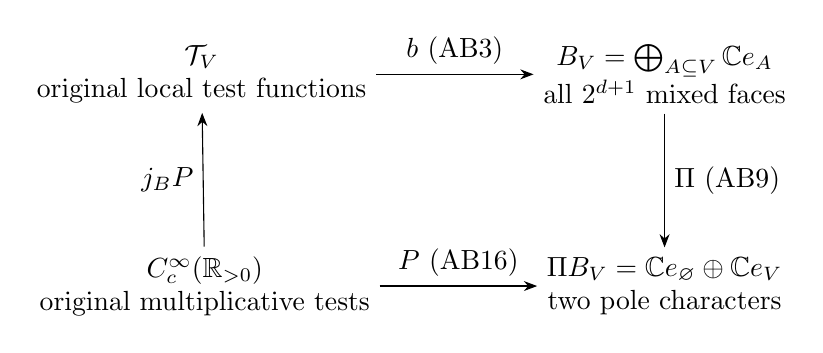
\begin{tikzpicture}[>=Stealth, node distance=17mm and 20mm,
 every node/.style={align=center}]
\node (tests) {$\mathcal T_V$\\original local test functions};
\node[right=of tests] (faces) {$B_V=\bigoplus_{A\subseteq V}\C e_A$\\all $2^{d+1}$ mixed faces};
\node[below=of faces] (poles) {$\Pi B_V=\C e_\varnothing\oplus\C e_V$\\two pole characters};
\node[left=of poles] (multiplicative) {$C_c^\infty(\R_{>0})$\\original multiplicative tests};
\draw[->] (tests)--node[above] {$b$ (AB3)} (faces);
\draw[->] (faces)--node[right] {$\Pi$ (AB9)} (poles);
\draw[->] (multiplicative)--node[above] {$P$ (AB16)} (poles);
\draw[->] (multiplicative)--node[left] {$j_BP$} (tests);
\end{tikzpicture}
\caption{The mixed boundary calculation, with its actual maps. The square
commutes by (AB19). Every proper face has the character (AB5) and the
contracting homotopy (AB12); both surviving faces enter the pole pairing
(AB17). This diagram concerns the computed boundary quotient, not an
asserted replacement for the full zeta cohomology.}
\end{figure}

\subsection{Passing to every prime with the original reference functions}
The finite-place calculation has a specific global continuation. If
$F\subset F'$ and $V'=\{\infty\}\sqcup F'$, the original restricted
Schwartz tensor product uses $\mathbf1_{\Z_p}$ at $p\in F'\setminus F$.
Its evaluation and integral are both one for the fixed Haar measure.
The induced injective boundary map is therefore
\[
 j_{FF'}:B_V\longrightarrow B_{V'},\qquad
 c\longmapsto c\otimes\bigotimes_{p\in F'\setminus F}(e_0+e_1).
 \tag{AB20}
\]
There is no omitted scalar in this formula. The ordering of the added
tensor factors is the ordering of the places. These maps compose exactly
and commute with the original Fourier involutions. They are equivariant
for $\Gamma_F$, since its elements have absolute value one at each added
prime. Let
\[
 B_{\rm all}=\varinjlim_F B_{\{\infty\}\cup F}.
 \tag{AB21}
\]
The nonempty finite $F$ form a cofinal set, so the preceding results apply.
The whole group $\Q^\times$ acts on this direct limit: for any $\gamma$,
first enlarge $F$ to include its prime factors and then use (AB5).
Equivariance at every further enlargement proves independence of choices
and the group law. The restricted algebraic Schwartz space
\[
 \mathcal T_{\rm all}=\Sch(\R)\otimes
              \bigotimes_{p}'(\Sch(\Q_p),\mathbf1_{\Z_p})
 \tag{AB22}
\]
maps onto $B_{\rm all}$ by the $b_v$, because every finite-level map is
onto and their transition maps agree by (AB20). This is the original
reference-function convention of \cite[Section III]{Connes1998}.

\begin{theorem}[The global boundary quotient and its invariant vectors]
\label{thm:global-boundary}
Let $\pi_F:B_V\to\C^2$ take the empty and full coordinates, in that order.
The maps $\pi_F$ induce a surjective $\Q^\times$-invariant map
$\pi_{\rm all}:B_{\rm all}\to\C^2$, and
\[
 (B_{\rm all})_{\Q^\times}\xrightarrow[\ \pi_{\rm all}\ ]{\sim}\C^2,
 \qquad (B_{\rm all})^{\Q^\times}=0.
 \tag{AB23}
\]
The composite from $\mathcal T_{\rm all}$ is exactly
$f\mapsto(f(0),\int f)$ with its original adelic measure.
The two-dimensional quotient consequently has no equivariant linear
section into $B_{\rm all}$.
\end{theorem}
\begin{proof}
Each endpoint coordinate of (AB20) is the same endpoint coordinate of
$c$, so $\pi_{F'}j_{FF'}=\pi_F$. An element $\gamma\in\Q^\times$
can be tested in a stage containing all its prime factors. Both endpoint
characters there equal one by the product formula, proving invariance.
Surjectivity holds at any finite stage.

If $\pi_{\rm all}c=0$, represent $c$ at a finite stage. Its two endpoint
coordinates are zero, so it is a sum of proper-face basis vectors. For
each such vector the explicit identity following (AB10) expresses it as
$(D_p-I)$ of a vector at that same stage. Hence $c$ is in the span of
the coinvariant relations. Conversely invariance of $\pi_{\rm all}$
kills every such relation. This proves the quotient assertion.

For the invariant-vector assertion, let a nonzero $c$ be represented in
$B_V$. Choose a prime $p\notin F$ and view it in the next stage through
$j_{F,F\cup\{p\}}$. For each nonzero coefficient $c_A$, the two
extended faces $(A,0)$ and $(A,1)$ both have that same nonzero coefficient.
Under $p$, their eigenvalues are respectively
$p^{\mathbf1_{\infty\in A}}$ and
$p^{\mathbf1_{\infty\in A}-1}$. Exactly one equals one; the other is
$p$ or $p^{-1}$, and therefore differs from one. Different $A$ yield
different coordinate positions, so these nonzero changes cannot cancel.
Thus $(D_p-I)j_{F,F\cup\{p\}}c\ne0$. All later maps are injective, so
this remains nonzero in the direct limit. No nonzero vector is invariant.
If an equivariant section from the trivial representation $\C^2$ existed,
its image would consist of invariant vectors, contradicting this result.
Finally both evaluation and integral multiply by one on each reference
factor, proving the formula on pure tensors and then on finite sums.
\end{proof}

Both pairings can be tracked through these same maps. From (AB15),
for $r=|F'\setminus F|$ one obtains
\[
 \mathscr B_{V'}(j_{FF'}c,j_{FF'}d)=2^r\mathscr B_V(c,d),
 \qquad
 \mathscr B_{V'}(\Pi_{F'}j_{FF'}c,\Pi_{F'}j_{FF'}d)
 =\mathscr B_V(\Pi_Fc,\Pi_Fd).
 \tag{AB24}
\]
For the first equality each added local factor $(1,1)$ has value two
under its complement pairing, so tensoring gives exactly $2^r$.
For the second equality both sides equal
$\overline{c_\varnothing}d_V+\overline{c_V}d_\varnothing$.
Consequently the pole pairing (AB17) is compatible at every stage,
whereas the full mixed pairing has the explicitly calculated factor
$2^r$. No unrecorded change of measure or scalar has been made.

This establishes a global quotient from the actual local test spaces.
It also identifies exactly what passage to all primes changes: the
finite invariant endpoint vectors do not survive as global invariant
vectors, while the two pole coordinates survive as a quotient. The
kernel of that quotient, including its original arithmetic cohomology,
is retained as a separate mathematical object throughout the construction.

% END COMPLETE PROOF SOURCE: 06_adelic_boundary.tex


% BEGIN COMPLETE PROOF SOURCE: 11_mixed_extension_prime_trace.tex
\section{The mixed-support extension and its arithmetic determinant}
\label{sec:mixed-extension-trace}
The full mixed boundary constructed above contains more information than its
two-dimensional quotient. We now compute a nonzero extension class, its local
differentials, and their exact contribution to the prime terms of Weil's
formula. The primes and their absolute values are those of the original
arithmetic stratum $V(e)\subset\Spec G(\Z)$. All tests, Haar measures and
the prime terms $W_p$ remain those of Section~\ref{sec:prime-faces-weil}.
The classical trace-formula source is Connes
\cite[Section III and Section V]{Connes1998}, and the exact explicit-formula
conventions are those read in \cite[\texttt{wp}, \texttt{arch}]{Connes2026}.
The extension and determinant calculations below are proved here.

\subsection{A nonzero class carried by all the mixed faces}
For a finite set $F$ of primes, including $F=\varnothing$, write
$B_F=\bigotimes_{v\in\{\infty\}\sqcup F}\C^2$ as in (AB2).
Use exactly the bonding maps
\[
 j_{FF'}c=c\otimes\bigotimes_{p\in F'\setminus F}(e_0+e_1).
 \tag{ME1}
\]
They come from the original reference function $\mathbf1_{\Z_p}$,
whose value at zero and integral both equal one. Put
$B=\varinjlim_F B_F$. For $\gamma\in\Q^\times$, choose $F$ containing
every prime factor of its numerator and denominator. The action on $B_F$ is
$D_\gamma e_A=\chi_A(\gamma)e_A$ with (AB5), and enlarging $F$ makes
this an action on $B$.

There is a canonical complex-parameter deformation of this particular
action: because all its eigenvalues are positive real numbers, define
\[
 D_\gamma(s)e_A=\exp(s\log\chi_A(\gamma))e_A,
 \qquad s\in\C.
 \tag{ME2}
\]
The logarithm here is the real logarithm of a positive number. Thus
$D_\gamma(1)=D_\gamma$, no eigenvalue or absolute value is changed, and
$D_{\gamma\eta}(s)=D_\gamma(s)D_\eta(s)$ follows from the real logarithm's
additivity. The new coordinates in (ME1) have character one on
$\Gamma_F$, proving compatibility for every $s$. Denote this module by
$B(s)$. Fourier complementation satisfies
$CD_\gamma(s)C=D_{\gamma^{-1}}(s)$.

The two endpoint coordinates give a surjection
$\epsilon:B(s)\to\C^2$, independent of $F$ and $s$. Define
$K(s)=\ker\epsilon$. The target has the trivial rational action, by the
product formula. Hence there is an exact sequence of actual modules
\[
 0\longrightarrow K(s)\longrightarrow B(s)
 \xrightarrow{\epsilon}\C^2\longrightarrow0.
 \tag{ME3}\label{eq:ME-extension}
\]
Let $b_0,b_1\in B(s)$ be the two basis vectors at $F=\varnothing$;
they give the specified vector-space section of $\epsilon$.

\begin{theorem}[Explicit global mixed-support extension]
\label{thm:ME-extension}
For $\Re s>0$, $B(s)^{\Q^\times}=0$, and (ME3) has no equivariant
section. Its two connecting cocycles are
\[
 c_j(\gamma;s)=D_\gamma(s)b_j-b_j\in K(s),\qquad j=0,1.
 \tag{ME4}
\]
They determine linearly independent elements of
$H^1(\Q^\times,K(s))$. For $\gamma$ with prime factors in $F$, their
complete coordinates are
\begin{align}
 c_0(\gamma;s)&=
 \sum_{A\subseteq F}
 \left(\prod_{p\in A}|\gamma|_p^s-1\right)e_A,\tag{ME5}\\
 c_1(\gamma;s)&=
 \sum_{A\subseteq F}
 \left(|\gamma|_\infty^s\prod_{p\in A}|\gamma|_p^s-1\right)
 e_{\{\infty\}\cup A}.\tag{ME6}
\end{align}
In particular, on the original four faces at $\{\infty,p\}$,
\[
 c_0(p;s)=(p^{-s}-1)e_{\{p\}},\qquad
 c_1(p;s)=(p^s-1)e_{\{\infty\}}.
 \tag{ME7}\label{eq:ME-local-cocycle}
\]
These are nonzero mixed-face coordinates, not endpoint coordinates.
\end{theorem}
\begin{proof}
At stage $F$, (ME1) sends $b_0$ to $\sum_{A\subset F}e_A$ and
$b_1$ to $\sum_{A\subset F}e_{\{\infty\}\cup A}$. Acting diagonally
and subtracting gives (ME5)--(ME6). Their empty and full coordinates vanish,
the latter by the full product formula, so they lie in $K(s)$.

If $z\ne0$ is represented in $B_F$, choose a prime $p\notin F$.
Its image in $B_{F\cup\{p\}}$ has equal coefficients $z_A$ on $A$
and $A\cup\{p\}$. If $\infty\notin A$, the first has eigenvalue one
under $D_p(s)$ and the second has eigenvalue $p^{-s}$. If
$\infty\in A$, the eigenvalues are $p^s$ and one. Since $\Re s>0$,
the nonunit eigenvalue never equals one. At least one nonzero coefficient
is therefore changed. Every bonding map is injective, since tensoring by
the nonzero vector $e_0+e_1$ is injective. Thus $z$ cannot become invariant
at a later stage either. This proves the assertion about invariants and
excludes an equivariant section.

Multiplying the operators gives
$c_j(\gamma\eta)=D_\gamma(s)c_j(\eta)+c_j(\gamma)$, the cocycle
identity. Suppose $a_0c_0+a_1c_1$ is a coboundary
$D_\gamma(s)k-k$ with $k\in K(s)$. Then
$a_0b_0+a_1b_1-k$ is invariant. The preceding argument forces it to
vanish, and applying $\epsilon$ gives $(a_0,a_1)=0$.
This proves linear independence, using the definition of group
cohomology rather than an assumed vanishing or comparison theorem.
Specializing (ME5)--(ME6) to $F=\{p\}$ proves (ME7).
\end{proof}

At the original value $s=1$, the complement pairing of (AB15) gives
\[
 \mathscr B(c_0(p;1),c_1(p;1))
 =(p^{-1}-1)(p-1)=-(\sqrt p-1/\sqrt p)^2.
 \tag{ME8}
\]
This follows by pairing the two complementary face vectors, each with
coefficient one in the original pairing. It is an evaluated pairing of
the extension, not an assignment of a Weil sign to every test.

\subsection{The determinant of the actual local differential}
Restrict to the infinite cyclic subgroup generated by $p$ and the
invariant mixed-face subspace
\[
 M_p=\C e_{\{p\}}\oplus\C e_{\{\infty\}}\subset B_{\{p\}}.
 \tag{ME9}
\]
The standard two-term cochain complex in this case is obtained directly
from the free resolution
$0\to\C[t,t^{-1}]\xrightarrow{t-1}\C[t,t^{-1}]\to\C\to0$.
The first map is injective because a Laurent polynomial ring is a domain;
the cokernel is evaluation at one. Applying module Hom proves, in the
displayed order of basis vectors, that the differential is
\[
 d_p(s)=D_p(s)-I=
 \begin{pmatrix}p^{-s}-1&0\\0&p^s-1\end{pmatrix}:
 M_p\longrightarrow M_p.
 \tag{ME10}\label{eq:ME-differential}
\]
It is the same matrix that evaluates the two cocycles (ME7) on the
generator. It is invertible for $\Re s>0$. Its determinant, with both
orientations and the original ordered basis retained, is
\[
 \det d_p(s)=(p^{-s}-1)(p^s-1)
 =-p^s(1-p^{-s})^2.
 \tag{ME11}
\]

For clarity, the determinant-line calculation can be specified without a
torsion convention: in a one-dimensional complex
$L^0\xrightarrow{a}L^1$ with named bases, the map
$\det L^0\otimes(\det L^1)^*\to\C$ induced by the differential
sends the named tensor to $a$. Its inverse scalar is $a^{-1}$.
For the finite-place line in (ME10) this scalar is
$(p^{-s}-1)^{-1}=-(1-p^{-s})^{-1}$. Thus the exact arithmetic Euler
factor is
\[
 Z_p(s)=\frac1{1-p^{-s}}
 =-\bigl(\det d_p(s)|_{\C e_{\{p\}}}\bigr)^{-1}.
 \tag{ME12}\label{eq:ME-euler-torsion}
\]
The minus sign is displayed, not absorbed into a basis change. The
complementary line has inverse determinant
$(p^s-1)^{-1}=p^{-s}Z_p(s)$. Their product is therefore
$-p^{-s}Z_p(s)^2$, in agreement with (ME11).

The extraction of this local line has an exact chain map from all the
finite-place data. Fix $p\in F$. Define
$r_{F,p}:B_F(s)\to B_{\{p\}}(s)$ by retaining the coefficients of
$e_A$ only when $A\subseteq\{\infty,p\}$ and setting every spectator
coordinate to the evaluation component. Then
\[
 r_{F,p}D_p(s)=D_p(s)r_{F,p},\qquad
 r_{F,p}j_{\{p\},F}=I.
 \tag{ME13}
\]
Indeed $|p|_q=1$ at every spectator prime $q$, and exactly the empty
spectator choice survives the projection of the tensor in (ME1).
Projection of the full Koszul complex (AB11) to degrees zero and one
along the $p$ direction, followed by $r_{F,p}$, is a cochain map to
the cyclic complex: all other exterior generators project to zero.
Finally projection onto the two mixed faces and then onto the finite-place
line commutes with $D_p(s)-I$. These identities prove the whole chain map
that extracts (ME12). They do not identify this determinant with the
torsion of the entire higher-rank Koszul complex.

\begin{proposition}[The full prime product in its domain of convergence]
For $\Re s>1$, the product of the factors (ME12), one for each original
finite prime, converges absolutely and equals
\[
 \prod_p Z_p(s)=\sum_{n\ge1}n^{-s}=\zeta(s).
 \tag{ME14}
\]
\end{proposition}
\begin{proof}
Write $\sigma=\Re s>1$. Then
$\sum_p\sum_{m\ge1}p^{-m\sigma}/m
\le(1-2^{-\sigma})^{-1}\sum_{n\ge2}n^{-\sigma}<\infty$,
so the logarithms of the product converge absolutely.
For a finite set of primes the geometric-series expansion is absolutely
convergent and enumerates exactly the positive integers with prime factors
in that set, once each by unique prime factorization. Its omitted terms
are dominated by the summable series $\sum n^{-\sigma}$. Passing to all
primes proves (ME14). This derivation concerns the convergent Euler
product; it makes no assertion about zeros in its meromorphic continuation.
\end{proof}

\subsection{An exact receiver in the original Weil prime term}
Define the logarithmic derivative of the same finite-place differential by
\[
 L_p(s)=-\frac{d}{ds}\log Z_p(s)
 =\frac{(\log p)p^{-s}}{1-p^{-s}}
 =(\log p)\sum_{m\ge1}p^{-ms},\qquad\Re s>0.
 \tag{ME15}\label{eq:ME-log-derivative}
\]
There is no branch issue: the first expression means $-Z_p'/Z_p$,
and the last equality is an absolutely convergent geometric series.
Let $g\in C_c^\infty(\R_{>0})$, let $h=g*g^*$ use the original
multiplicative Haar measure $dx/x$, and put
$\widehat g(t)=\int_0^\infty g(x)x^{-it}dx/x$. Thus
$\widehat h(t)=|\widehat g(t)|^2$ for real $t$.

\begin{theorem}[Mixed-differential formula for every prime-power term]
\label{thm:ME-Weil-prime}
The exact prime term of the original explicit formula is
\begin{align}
 W_p(h)&=(\log p)\sum_{m\ge1}p^{-m/2}
       \bigl(h(p^m)+h(p^{-m})\bigr)\notag\\
 &=\frac1{2\pi}\int_\R |\widehat g(t)|^2
 \left(L_p(\tfrac12+it)+L_p(\tfrac12-it)\right)\,dt.
 \tag{ME16}\label{eq:ME-Weil-prime}
\end{align}
Consequently, with $r=p^{-1/2}$ and
$P_r(\theta)=(1-r^2)/(1-2r\cos\theta+r^2)$,
\[
 W_p(g*g^*)=\frac{\log p}{2\pi}\int_\R
 |\widehat g(t)|^2\bigl(P_{p^{-1/2}}(t\log p)-1\bigr)\,dt.
 \tag{ME17}\label{eq:ME-poisson}
\]
Both pole terms, every prime power and the Archimedean term are retained
in the resulting finite-place Weil functional:
\begin{align}
 D_F(g*g^*)={}&\mathscr B(Pg,Pg)-W_\infty(g*g^*)\notag\\
 &+\sum_{p\in F}(\log p)\left(
 \|g\|_{L^2(dx/x)}^2-
 \frac1{2\pi}\int_\R|\widehat g(t)|^2
 P_{p^{-1/2}}(t\log p)\,dt\right).
 \tag{ME18}\label{eq:ME-complete-prime-receiver}
\end{align}
Here $P$ is precisely the two-pole map (AB16); no new source or metric
has been substituted for the original test.
\end{theorem}
\begin{proof}
In logarithmic coordinates the Fourier inversion formula is
$h(e^u)=(2\pi)^{-1}\int\widehat h(t)e^{itu}dt$.
The two series in (ME15), evaluated at $1/2\pm it$, have total absolute
sum at most $2(\log p)p^{-1/2}/(1-p^{-1/2})$ uniformly in $t$.
Since $\widehat h$ is a Schwartz function, absolute integrability justifies
interchanging the integrals and the series. Fourier inversion at
$u=\pm m\log p$ proves (ME16), including the factor $1/(2\pi)$.
For $z=re^{-i\theta}$ direct multiplication gives
\[
 \frac{z}{1-z}+\frac{\bar z}{1-\bar z}
 =\frac{2r\cos\theta-2r^2}{1-2r\cos\theta+r^2}
 =P_r(\theta)-1.
 \tag{ME19}
\]
This proves (ME17). Finally the full pole pairing was computed in (AB17),
$D_F$ is the original pole term minus the Archimedean term and minus
$\sum_{p\in F}W_p$, and Fourier Plancherel in the same logarithmic
coordinate gives $(2\pi)^{-1}\int|\widehat g|^2=\|g\|^2$.
Substitution proves (ME18).
\end{proof}

Each Poisson energy in (ME18) is positive for $g\ne0$: its integrand is
nonnegative, $P_r$ is strictly positive, and Plancherel excludes a zero
Fourier transform for nonzero $g$. Its subtraction from $\|g\|^2$ has
the exact sign already tested by the two-bump examples of
Theorem~\ref{thm:prime-face-signs}. Thus the formula retains the
competing energies; it does not replace their difference by a positivity
assertion. If $\supp g\subset[\lambda^{-1},\lambda]$ and
$p>\lambda^2$, every $h(p^{\pm m})$ vanishes, so (ME16) proves that
the corresponding Poisson energy is \emph{exactly} $\|g\|^2$.
Consequently (ME18) becomes the full prime return at
$F=\{p:p\le\lambda^2\}$, without summing separately divergent
norm and Poisson-energy series.

\begin{figure}[ht]
\centering
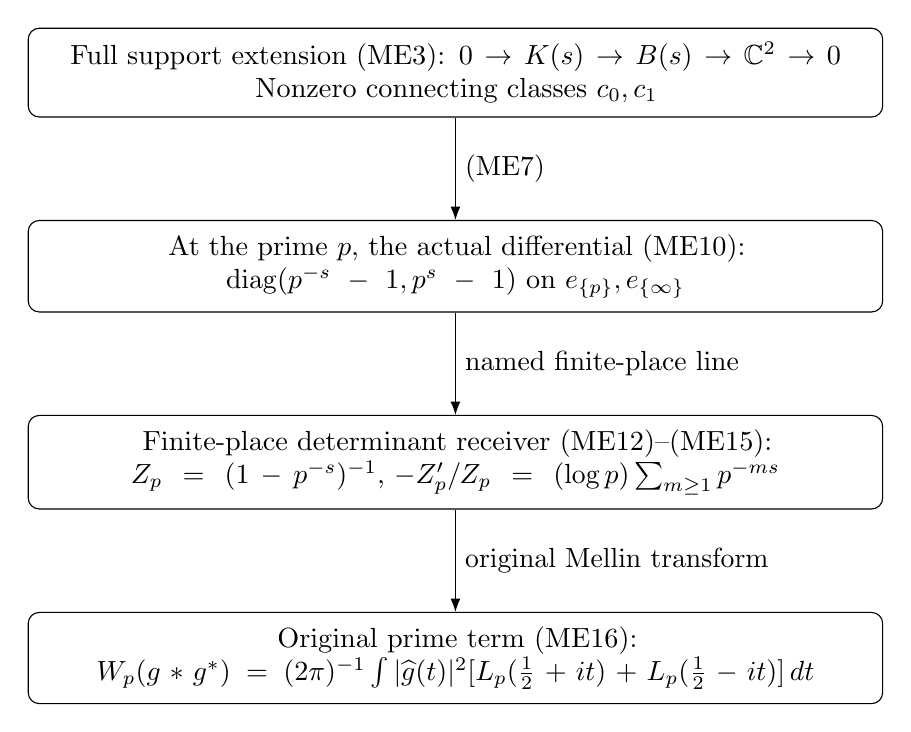
\begin{tikzpicture}[node distance=13mm, every node/.style={align=center},
 box/.style={draw,rounded corners,text width=105mm,inner sep=5pt}]
\node[box] (ext) {Full support extension (ME3):
$0\to K(s)\to B(s)\to\C^2\to0$\\
Nonzero connecting classes $c_0,c_1$};
\node[box,below=of ext] (diff) {At the prime $p$, the actual differential (ME10):\\
$\operatorname{diag}(p^{-s}-1,p^s-1)$ on
$e_{\{p\}},e_{\{\infty\}}$};
\node[box,below=of diff] (log) {Finite-place determinant receiver (ME12)--(ME15):\\
$Z_p=(1-p^{-s})^{-1}$,
$-Z_p'/Z_p=(\log p)\sum_{m\ge1}p^{-ms}$};
\node[box,below=of log] (weil) {Original prime term (ME16):\\
$W_p(g*g^*)=(2\pi)^{-1}\int|\widehat g(t)|^2
 [L_p(\frac12+it)+L_p(\frac12-it)]\,dt$};
\draw[-{Latex}] (ext)--node[right]{(ME7)}(diff);
\draw[-{Latex}] (diff)--node[right]{named finite-place line}(log);
\draw[-{Latex}] (log)--node[right]{original Mellin transform}(weil);
\end{tikzpicture}
\caption{The calculated route from all support faces to each arithmetic
prime-power contribution. The complementary line and its minus sign remain
in (ME11)--(ME12); the local extraction is the explicit chain map (ME13).
Theorem~\ref{thm:ME-Weil-prime} proves the last arrow in the conventions of
Connes \cite{Connes1998,Connes2026}. These are exact maps and equalities,
not a diagram asserting the still-unproved full Weil positivity.}
\end{figure}

The use of the new support geometry in this section is specific: a global
nonsplit mixed extension supplies a local differential; its determinant
and logarithmic derivative supply the Euler factor and the complete
prime-power term. Ordinary endpoint coinvariants alone would not retain
that differential. The remaining calculation for the RH programme is the
pairing of the full interior cohomology with these retained relative terms
and the Archimedean term in (ME18). No coefficient of an earlier large-degree
determinant has been used to stand in for that pairing.

% END COMPLETE PROOF SOURCE: 11_mixed_extension_prime_trace.tex


% BEGIN COMPLETE PROOF SOURCE: 12_relative_prime_recollement.tex
\section{Relative cohomology at the full supported prime}\label{sec:relative-prime-recollement}


\subsection{The full space and the receiving categories}

Let $X$ be a nonempty irreducible topological space. Put
$Y=X^+=X\sqcup\{\eta_\tau\}$. Its nonempty opens are the singleton
$\{\eta_\tau\}$ and $U^+=U\cup\{\eta_\tau\}$ for nonempty open
$U\subset X$. Write $i:X\hookrightarrow Y$ and
$j:\{\eta_\tau\}\hookrightarrow Y$. All nonempty opens of $X$ intersect.
In the first four parts of this chapter, sheaves have values in modules over a fixed commutative
coefficient ring $\Lambda$; taking $\Lambda=\mathbb Z$ gives abelian
sheaves. These are sheaves on the entire underlying prime space.
They are not automatically additive-group modules over its semiring
structure sheaf. Section~\ref{sec:actual-semiring} proves the exact
distinction and the resulting morphisms.

For a module $B$, let $cB$ be the sheaf on $X$ with value $B$ on every
nonempty open and identity restriction between such opens. This is a
sheaf because any two members of a nonempty open cover intersect, so
compatible locally constant values agree. Define
\[
 g\mathcal A=\varinjlim_{\varnothing\ne U\subset X}\mathcal A(U),
 \qquad \epsilon_{\mathcal A}:\mathcal A\longrightarrow c(g\mathcal A).
 \tag{RP1}\label{eq:generic-functor}
\]
The indexing order is restriction to smaller nonempty opens. It is
filtered by irreducibility. If $X$ has a generic point $\xi$, then every
nonempty open contains $\xi$, and $g\mathcal A=\mathcal A_\xi$.

\begin{lemma}[Exact generic-section adjunction]\label{lem:generic}
The functors $g$ and $c$ are exact, $g$ is left adjoint to $c$, and
$gcB=B$. In particular $c$ preserves injective modules as injective
sheaves, and
\[
 R\Gamma(X,cB)=B[0].
 \tag{RP2}\label{eq:constant-cohomology}
\]
\end{lemma}
\begin{proof}
A morphism $\mathcal A\to cB$ is a family of maps
$\mathcal A(U)\to B$ agreeing under all restrictions. The filtered
colimit is exactly their universal receiving module, proving the
adjunction. The assertions $gcB=B$ and exactness of $c$ follow from its
displayed sections or stalks. To check surjectivity of $g$ on an
epimorphism of sheaves, represent a generic section by a section on a
nonempty $U$. Sheaf surjectivity supplies a lift on an open cover of
$U$; choose a nonempty member and take its generic germ. For exactness
in the middle, if a section has zero image as a generic germ, restrict
to a nonempty smaller open on which its image is zero, then use the
kernel sheaf. This proves exactness of $g$.

The adjunction and exactness of $g$ imply that $c$ takes injectives to
injectives: applying $\Hom(-,cI)=\Hom(g(-),I)$ to an exact sequence is
exact if $I$ is injective. Apply $c$ to an injective resolution of $B$.
It remains an injective resolution, and its sections on $X$ are the
original resolution. This proves \eqref{eq:constant-cohomology}.
\end{proof}

\begin{theorem}[All sheaves and all gluing maps]\label{thm:triples}
The category $\Sh(Y,\Lambda)$ is equivalent to the category of triples
\[
 \mathcal F=(\mathcal A,B,\phi),\qquad
 \phi:\mathcal A\longrightarrow cB,
 \tag{RP3}\label{eq:triples}
\]
where $\mathcal A\in\Sh(X,\Lambda)$ and $B\in\Lambda\text{-}\mathrm{Mod}$.
Its sections are $\mathcal F(U^+)=\mathcal A(U)$ and
$\mathcal F(\{\eta_\tau\})=B$; restriction to the singleton is
$\phi_U$. A morphism is a pair $(a,b)$ satisfying
$\phi'a=c(b)\phi$. Kernels and cokernels are computed componentwise.
Equivalently, the gluing is an arbitrary map
$\overline\phi:g\mathcal A\to B$.
\end{theorem}
\begin{proof}
For a sheaf $\mathcal F$ on $Y$ put $B=\mathcal F(\{\eta_\tau\})$ and
$\mathcal A(U)=\mathcal F(U^+)$ on nonempty opens. If $U$ is covered
by nonempty opens $U_a$, their pairwise intersections are nonempty,
and $(U_a\cap U_b)^+=U_a^+\cap U_b^+$. Thus the sheaf axiom for
$\mathcal F$ is exactly the sheaf axiom for these values on $X$.
Restriction to the singleton gives $\phi$. This $\mathcal A$ is
$i^*\mathcal F$, since $U^+$ is the smallest open of $Y$ containing $U$
and no further sheafification changes the displayed sheaf.

Conversely the displayed formulas for a triple define a sheaf.
On a cover of $U^+$, sections on nonempty arithmetic parts glue by the
sheaf axiom for $\mathcal A$; their images in $B$ agree, and hence
also agree with any section on a singleton member of the cover.
The singleton case is immediate. The two constructions are inverse.
The compatibility equation is precisely restriction compatibility.
Since $c$ is exact, both a componentwise kernel and a componentwise
cokernel inherit the indicated arrow and satisfy the categorical
universal property. The last assertion is Lemma~\ref{lem:generic}.
\end{proof}

\subsection{The six elementary functors and their derived terms}

\begin{theorem}[Explicit recollement]\label{thm:recollement}
In triple notation the functors are
\[
\begin{array}{lll}
 i^*(\mathcal A,B,\phi)=\mathcal A,&
 i_*\mathcal A=(\mathcal A,0,0),&
 i^!(\mathcal A,B,\phi)=\ker\phi,\\[2pt]
 j^*(\mathcal A,B,\phi)=B,&
 j_!B=(0,B,0),&
 j_*B=(cB,B,\mathrm{id}).
\end{array}
 \tag{RP4}\label{eq:six-functors}
\]
The adjunctions are $i^*\dashv i_*\dashv i^!$ and
$j_!\dashv j^*\dashv j_*$. All displayed functors except possibly
$i^!$ are exact. There is in addition an exact left adjoint to $i^*$,
\[
 U\mathcal A=(\mathcal A,g\mathcal A,\epsilon_{\mathcal A}),
 \qquad U\dashv i^*.
 \tag{RP5}\label{eq:universal-coupling}
\]
For any triple, there is a canonical short exact sequence
\[
 0\longrightarrow j_!B\longrightarrow\mathcal F
 \longrightarrow i_*\mathcal A\longrightarrow0.
 \tag{RP6}\label{eq:gluing-extension}
\]
\end{theorem}
\begin{proof}
A map $\mathcal F\to i_*\mathcal C$ is precisely a map
$\mathcal A\to\mathcal C$. A map $i_*\mathcal C\to\mathcal F$
is a map $\mathcal C\to\mathcal A$ whose composite with $\phi$ is zero,
hence a map to $\ker\phi$. A map $j_!D\to\mathcal F$ is any map
$D\to B$. A map $\mathcal F\to j_*D$ has its arithmetic component
forced to be $c(b)\phi$, so is any map $b:B\to D$. These calculations
prove the four adjunctions and all formulas. Exactness follows from
componentwise exactness and exactness of $c$.

A map $U\mathcal C\to\mathcal F$ has arithmetic part
$a:\mathcal C\to\mathcal A$ and must have generic part the unique map
$g\mathcal C\to B$ corresponding to $\phi a$ under the adjunction
of Lemma~\ref{lem:generic}. This proves $U\dashv i^*$; its exactness
follows from exactness of $g$. Finally the maps in
\eqref{eq:gluing-extension} have components $(0,\mathrm{id}_B)$ and
$(\mathrm{id}_{\mathcal A},0)$, proving its exactness.
\end{proof}

Complexes use cohomological degrees: $B[-1]$ has $B$ in degree one.
All derived statements below can be read in the bounded-below derived
categories. No assertion requires an unbounded resolution convention.

\begin{theorem}[Derived closed restriction and relative cohomology]
\label{thm:derived}
For $\mathcal F=(\mathcal A,B,\phi)$ one has canonical identifications
\[
 Ri^!\mathcal F\simeq
 [\mathcal A\xrightarrow{\phi}cB]
 =\operatorname{Cone}(\phi)[-1],
 \tag{RP7}\label{eq:derived-i-shriek}
\]
where the two entries are in degrees zero and one. Thus
$i^!\mathcal F=\ker\phi$, $R^1i^!\mathcal F=\coker\phi$, and
$R^ni^!\mathcal F=0$ for $n\ge2$.
Furthermore
\[
 R\Gamma(Y,\mathcal F)=R\Gamma(X,\mathcal A),\qquad
 R\Gamma_X(Y,\mathcal F)
 \simeq\operatorname{Cone}\bigl(R\Gamma(X,\mathcal A)\to B\bigr)[-1].
 \tag{RP8}\label{eq:relative-cohomology}
\]
Here $R\Gamma_X(Y,-)$ means $R\Gamma(X,Ri^!(-))$, the derived functor
of sections with support in the closed subset $X$. The corresponding
localization triangle is
\[
 i_*Ri^!\mathcal F\longrightarrow\mathcal F
 \xrightarrow{(\phi,\mathrm{id})}j_*B\longrightarrow i_*Ri^!\mathcal F[1].
 \tag{RP9}\label{eq:localization-triangle}
\]
\end{theorem}
\begin{proof}
There are enough injectives in the triple category. Indeed embed
$\mathcal A$ into an injective sheaf $I$ and $B$ into an injective
module $J$. The map
\[
 (\mathcal A,B,\phi)\longrightarrow i_*I\oplus j_*J
\]
with arithmetic component $(\mathcal A\hookrightarrow I,c(B\hookrightarrow
J)\phi)$ and generic component $B\hookrightarrow J$ is injective.
The target is injective because $i_*$ and $j_*$ are right adjoints
of exact functors.

If $\mathcal I=(\mathcal A_I,B_I,\phi_I)$ is injective, then
$\phi_I$ is split surjective. To see this, the monomorphism
$j_!B_I\hookrightarrow j_*B_I$ and the map $j_!B_I\to\mathcal I$
with generic part the identity extend to a map $j_*B_I\to\mathcal I$.
Its arithmetic part is a right inverse of $\phi_I$. Also
$\ker\phi_I$ is injective on $X$ because $i^!$ is right adjoint to the
exact functor $i_*$. The functors $i^*$ and $j^*$ preserve injectives:
their respective left adjoints $U$ and $j_!$ are exact.

For an injective resolution of $\mathcal F$, therefore, there is a
termwise split exact sequence of complexes
$0\to i^!\mathcal I^\bullet\to i^*\mathcal I^\bullet
\to c(j^*\mathcal I^\bullet)\to0$. The latter two complexes resolve
$\mathcal A$ and $cB$ by injectives. Its kernel computes $Ri^!$ and
is the indicated shifted cone. This proves \eqref{eq:derived-i-shriek}.
The same termwise calculation in the triple category proves
\eqref{eq:localization-triangle}.

Ordinary global sections equal $\Gamma(X,\mathcal A)$, and $i^*$
preserves injectives, proving the first identification in
\eqref{eq:relative-cohomology}. Apply $R\Gamma(X,-)$ to
\eqref{eq:derived-i-shriek} and use
\eqref{eq:constant-cohomology} for the second. At degree zero the
kernel is exactly the sections whose restriction to the open point
is zero, which proves the stated support interpretation.
\end{proof}

\begin{corollary}[A nonzero relative object and its connecting map]
\label{cor:boundary}
For every nonzero $B$, the sheaf $j_!B$ is nonzero and satisfies
\[
 R\Gamma(Y,j_!B)=0,\qquad Ri^!j_!B=cB[-1],\qquad
 R\Gamma_X(Y,j_!B)=B[-1].
 \tag{RP10}\label{eq:boundary-object}
\]
The sequence
\[
 0\longrightarrow j_!B\longrightarrow j_*B
 \longrightarrow i_*cB\longrightarrow0
 \tag{RP11}\label{eq:universal-boundary-extension}
\]
does not split. Its localization boundary identifies the actual module
$B$ at the new point with $H^1_X(Y,j_!B)$, with the sign convention
fixed by the order of maps in this exact sequence.
\end{corollary}
\begin{proof}
The three calculations are substitutions of $(0,B,0)$ into
Theorem~\ref{thm:derived}; its stalk at the new point proves it is
nonzero. A section of the surjection in
\eqref{eq:universal-boundary-extension} would be a triple morphism
$(cB,0,0)\to(cB,B,\mathrm{id})$ with arithmetic part the identity.
The compatibility equation would instead force that part to be zero.
This contradicts $B\ne0$. In the localization long exact sequence,
both global cohomology groups of $j_!B$ adjoining this boundary vanish,
so the boundary $B\to H^1_X(Y,j_!B)$ is the stated isomorphism.
\end{proof}

\subsection{Cross extensions, relative traces, and exact pairing maps}

\begin{theorem}[The new cross-extension groups]\label{thm:cross-ext}
For $n\ge1$,
\[
 \Ext_Y^n(i_*\mathcal A,j_!B)
 =\Ext_X^{n-1}(\mathcal A,cB)
 =\Ext_\Lambda^{n-1}(g\mathcal A,B),
 \qquad\Hom_Y(i_*\mathcal A,j_!B)=0.
 \tag{RP12}\label{eq:cross-extensions}
\]
All groups $\Ext_Y^n(j_!B,i_*\mathcal A)$ vanish, including $n=0$.
Under the degree-one identification in \eqref{eq:cross-extensions},
the class of \eqref{eq:gluing-extension} is exactly $\overline\phi$.
In particular the universal coupling $U\mathcal A$ represents
$\mathrm{id}_{g\mathcal A}$ and is nonsplit if $g\mathcal A\ne0$.
\end{theorem}
\begin{proof}
The exact functor $i_*$ and its right adjoint $i^!$ give, using injective
resolutions,
\[
\RHom_Y(i_*\mathcal A,j_!B)=\RHom_X(\mathcal A,Ri^!j_!B).
\]
Substitute
$Ri^!j_!B=cB[-1]$. The exact adjunction $g\dashv c$, with $c$ preserving
injectives, then gives
$\RHom_X(\mathcal A,cB)=\RHom_\Lambda(g\mathcal A,B)$.
This proves \eqref{eq:cross-extensions}. For the reverse direction,
use $j_!\dashv j^*$, exactness of $j_!$, and $j^*i_*=0$.

The extension \eqref{eq:gluing-extension} is the pullback of
\eqref{eq:universal-boundary-extension} along
$i_*\phi:i_*\mathcal A\to i_*cB$: the fibre product has exactly the
triple $(\mathcal A,B,\phi)$. The universal sequence corresponds to
$\mathrm{id}_{cB}$ under the derived adjunction, fixing its sign;
pullback therefore corresponds to $\phi$, and then to
$\overline\phi$. For $U\mathcal A$ that map is the identity.
\end{proof}

For a scheme with generic point, \eqref{eq:cross-extensions} says exactly
that this direct cross-extension channel receives the generic stalk.
A sheaf whose generic stalk is zero has no such cross-extension.
This fact does not remove its other supported-prime data. The universal
coupling in Section~\ref{sec:principal-parts} gives the exact relative
object in which the quotients by those prime stalks occur.

\begin{proposition}[Full mapping complex]\label{prop:mapping-complex}
For $\mathcal F=(\mathcal A,B,\phi)$ and
$\mathcal F'=(\mathcal A',B',\phi')$, their derived mapping complex is
the fibre of
\[
 \RHom_X(\mathcal A,\mathcal A')\oplus\RHom_\Lambda(B,B')
 \longrightarrow\RHom_\Lambda(g\mathcal A,B'),
 \quad (a,b)\longmapsto\overline\phi'\,g(a)-b\,\overline\phi.
 \tag{RP13}\label{eq:mapping-fibre}
\]
\end{proposition}
\begin{proof}
Resolve the target by injective triples. Their arithmetic and generic
components are injective, as proved in Theorem~\ref{thm:derived}, and
their gluing arrows split. In each degree, the map of ordinary Hom
groups in \eqref{eq:mapping-fibre} is surjective: lift any map
$\mathcal A\to cB'_I$ through a splitting of $\phi'_I$ and take $b=0$.
Its kernel is exactly the compatible pairs defining a triple morphism.
Thus the complex of triple morphisms is the kernel of a surjective
map of complexes computing the displayed derived Homs. It is therefore
their homotopy fibre. Lemma~\ref{lem:generic} identifies the last
mapping complex with the stated module-valued one.
\end{proof}

Now take a coefficient field $k$. If $V,W$ are finite-dimensional
$k$-vector spaces, define
\[
 E(V,W)=\Ext_Y^1(i_*cV,j_!W)=\Hom_k(V,W).
 \tag{RP14}\label{eq:extension-pairing-space}
\]
There is a canonical perfect pairing
\[
 E(V,W)\times E(W,V)\longrightarrow k,
 \qquad (\phi,\psi)\longmapsto\tr_V(\psi\phi)=\tr_W(\phi\psi).
 \tag{RP15}\label{eq:extension-trace-pairing}
\]
Indeed matrices give both equal traces as
$\sum_{a,b}\phi_{ba}\psi_{ab}$; pairing a matrix unit with its transpose
shows nondegeneracy. This is a pairing of two explicitly identified
extension spaces with exchanged coefficient spaces. It is not a Yoneda
product through a nonexistent reverse cross-extension: those reverse
groups vanish by Theorem~\ref{thm:cross-ext}. For $k=\mathbb C$ and
specified positive Hermitian metrics, $\tr(\phi^*\psi)$ gives the
associated Hermitian form and $\tr(\phi^*\phi)=\sum_{a,b}|\phi_{ba}|^2$
in orthonormal bases. The metrics are additional data; topology alone
has not supplied them.

If $T:B\to B$ is an endomorphism of a finite-dimensional coefficient
space, its relative alternating trace is
\[
 \sum_n(-1)^n\tr\bigl(T\mid H_X^n(Y,j_!B)\bigr)=-\tr(T).
 \tag{RP16}\label{eq:relative-trace}
\]
This follows from \eqref{eq:boundary-object}, with its entire
cohomology in degree one. For two such sheaves the relative cup product
on their degree-one groups is zero: its target is
$H_X^2(Y,j_!(B\otimes_k D))=0$. Their tensor sheaf is $j_!(B\otimes D)$
because tensor products are computed on stalks and both arithmetic
stalks vanish. Thus the nonzero relative degree-one object and the
trace pairing \eqref{eq:extension-trace-pairing} have precise different
maps; identifying that trace pairing with a degree-two cup pairing
would give a false result.

\subsection{What the actual split structure sheaf retains}
\label{sec:actual-semiring}

Let $X$ now be an irreducible locally ringed space with nonzero local
rings. For a ring $R$, $\G(R)=\{\tau\}\sqcup R$, with $\tau$ the
additive identity and multiplicative absorber; write $e_R$ for its
supported coefficient zero. Supported addition and multiplication
are those of $R$, so $e_R+e_R=e_R$ and $e_Ra=e_R$ for every supported
$a$. The full semiring sheaf is
\[
 \mathcal S(U^+)=\G(\mathcal O_X(U)),\qquad
 \mathcal S(\{\eta_\tau\})=\mathbb B=\{0,1\},\quad1+1=1,
 \tag{RP17}\label{eq:semiring-sheaf}
\]
with support restriction to the singleton. Gluing is exact because
compatible sections agree in support at the common singleton; absent
sections glue to $\tau$, and supported coefficients glue in
$\mathcal O_X$. Its stalks are $\G(\mathcal O_{X,x})$ and $\mathbb B$.
The global section $e$ has arithmetic germs $e_{\mathcal O_{X,x}}$
and generic germ $1$ at the additional point. For an affine domain
$A$, the prime ideals of $\G(A)$ are $\{\tau\}$ and
$\{\tau\}\sqcup\mathfrak p$, $\mathfrak p\in\Spec A$: an ideal
containing a supported element contains $e_A$ and its supported
elements form a ring ideal by multiplication by $-1$. Products of
supported elements remain supported, proving primality of $\{\tau\}$.
This identifies $V(e)$ with the entire closed arithmetic stratum.

\begin{theorem}[Exact additive loss and joint recovery]
\label{thm:additive-loss}
The additive group completion of $\mathcal S$ is $i_*\mathcal O_X$.
Every sheaf of $\mathcal S$-semimodules with abelian-group addition is
uniquely an $i_*\mathcal O_X$-module; its generic stalk at
$\eta_\tau$ is zero. In particular neither nonzero $j_!B$ nor the
universal coupling $U\mathcal O_X$ with nonzero generic fibre is an
additive-group module over $\mathcal S$ with its stated unit action.

Nevertheless the joint map of semiring sheaves
\[
 (\chi,q):\mathcal S\longrightarrow j_*\mathbb B\times i_*\mathcal O_X
 \tag{RP18}\label{eq:joint-recovery}
\]
is injective. On $U^+$ it identifies the sections with $(0,0)$ and all
$(1,a)$, $a\in\mathcal O_X(U)$. Here $\chi$ retains support and $q$
retains the exact coefficient, including zero.
\end{theorem}
\begin{proof}
An additive map from $\G(R)$ to an abelian group sends $e_R$ to zero,
since $f(e_R)+f(e_R)=f(e_R)$. Its supported restriction is then a
group homomorphism from $R$, and the image of $\tau$ is zero. This
proves the universal group-completion property with quotient $R$.
At the Boolean stalk the relation $1+1=1$ kills its sole nonzero
generator, so its group completion is zero. Sheafification commutes
with this local universal property, yielding $i_*\mathcal O_X$.

For an additive-group semimodule, the relation
$e m+e m=e m$ gives $e m=0$. Thus its scalar action factors through
the indicated ring quotient. At the extra stalk $e=1$, so this says
$m=0$ for every element. This proves the module and nonexistence
assertions. In \eqref{eq:joint-recovery}, the absent section gives
$(0,0)$ and the supported zero gives $(1,0)$, which are distinct.
All other coefficients are distinguished by their second coordinate.
The same checks on operations prove it is a morphism and injective.
\end{proof}

\begin{proposition}[A multiplicative linearization that retains support]
\label{prop:monoid-linearization}
Let $\mathcal M$ be the sheaf of supported multiplicative elements of
$\mathcal S$: its values on $U^+$ are the multiplicative monoid of
$\mathcal O_X(U)$, including its supported zero, and its value on the
singleton is $\{1\}$. Let $\mathcal L=\mathbb Z[\mathcal M]$ be the
sheafification of its integral monoid algebra. Write $E=[e]$.
Then $E$ is a central idempotent, and
\[
 \mathcal L=E\mathcal L\oplus(1-E)\mathcal L,
 \qquad E\mathcal L\cong j_*\mathbb Z,
 \qquad (1-E)\mathcal L\cong i_*\mathcal C
 \tag{RP19}\label{eq:monoid-splitting}
\]
as rings with the two factor identities $E$ and $1-E$. Here
$\mathcal C_x=(1-[0])\mathbb Z[(\mathcal O_{X,x},\cdot)]$.
There is a surjection $\mathcal L\to i_*\mathcal O_X$, $[a]\mapsto a$,
whose kernel is the sheaf of ideals generated by
$[a+b]-[a]-[b]$. It kills the whole factor $E\mathcal L$.
The factor $E\mathcal L$ contains the canonical nonzero submodule
$j_!\mathbb Z$, and its quotient is $i_*\mathbb Z_X$ as in
\eqref{eq:universal-boundary-extension}.
\end{proposition}
\begin{proof}
Multiplicatively $e^2=e$ and $ea=e$ for every supported element.
Consequently $E^2=E$ and $E[a]=E$. The augmentation
$\varepsilon:\mathcal L\to j_*\mathbb Z$, $[a]\mapsto1$, is a ring
map. Multiplication by $E$ sends a section to its augmentation times
$E$, so its image is the free rank-one ring sheaf with identity $E$.
This proves its identification with $j_*\mathbb Z$. The complementary
factor has zero stalk at the added point, since $E=1$ there; the triple
description therefore places it on the closed arithmetic stratum and
gives its stated stalks. The central idempotent identity proves the
direct-product ring decomposition.

The quotient by the displayed additive relations has exactly the
universal property of a ring receiving the original supported addition
and multiplication. At an arithmetic stalk this is the original ring;
at the singleton the relation $[1]-[1]-[1]=-1$ makes the quotient zero.
Thus the quotient is precisely $i_*\mathcal O_X$. Taking $a=b=0$ gives
$-E$ among these relations, so its entire factor is killed.
The last assertion is \eqref{eq:universal-boundary-extension} on that
factor. All computations commute with restrictions and so prove the
sheaf assertions.
\end{proof}

This construction specifies both what survives and what is lost.
After tensoring with a coefficient field $k$, the $E$ factor is the
constant ring sheaf $j_*k$ on the full space $Y$. Its module category
is the category of all $k$-sheaves used above. The complementary
factor is supported on $X$. Every $\mathcal L\otimes k$-module splits
as $EM\oplus(1-E)M$, since these orthogonal idempotents sum to one;
the same decomposition of every map makes the module category a
product. Its cross-factor Hom and Ext groups are zero, by resolving
within each product component. Each supported scalar $[a]$ acts as
the identity on the $E$ factor. Thus its rank-one relative trace for
any such scalar is $-1$, by \eqref{eq:relative-trace}; the support
factor alone has not encoded a prime norm.

More specifically, if arithmetic coefficients are required to act
through $q$ and the additional fibre through $\varepsilon$, equivariance
of a gluing map would give
\[
 \phi(ea)=e\phi(a),\qquad\text{hence }0=\phi(a).
 \tag{RP20}\label{eq:coupling-obstruction}
\]
The exact space of couplings in the underlying abelian-sheaf category
is still $\Hom(g\mathcal A,B)$ by \eqref{eq:cross-extensions}; the
specified module compatibility selects its zero subspace. The universal
coupling \eqref{eq:universal-coupling} retains the entire arithmetic
sheaf and gives its identity generic coupling in that explicit receiving
category. The next calculation uses this object and does not assert
the incompatible semiring-module action.

\subsection{Principal parts at the supported primes}
\label{sec:principal-parts}

\begin{theorem}[Principal parts are the relative object of the new point]
\label{thm:principal-parts}
Let $X$ be an integral scheme with function field $F$, viewed with its
actual structure sheaf. Let $F_X=cF$ be its sheaf of rational functions
and define $\PP_X=F_X/\mathcal O_X$. For the canonical coupled abelian
sheaf
\[
 \mathcal U_X=U\mathcal O_X=(\mathcal O_X,F,
                      \mathcal O_X\hookrightarrow F_X)
 \tag{RP21}\label{eq:arithmetic-universal}
\]
one has
\[
 Ri^!\mathcal U_X=\PP_X[-1],\qquad
 (R^1i^!\mathcal U_X)_x=F/\mathcal O_{X,x}.
 \tag{RP22}\label{eq:principal-parts-relative}
\]
In particular a supported valuation-ring stalk $V$ contributes exactly
$F/V$. The ordinary generic stalk gives zero, while nonfield valuation
stalks give nonzero quotients. The maps are the original inclusions
$\mathcal O_{X,x}\hookrightarrow F$ and their exact cokernels.
\end{theorem}
\begin{proof}
An integral scheme embeds its structure sheaf in its function field:
on an affine domain chart, each local ring and each regular section
maps injectively into its fraction field, and these maps agree on
overlaps. Its generic stalk is $F$. Hence
\eqref{eq:universal-coupling} gives exactly
\eqref{eq:arithmetic-universal}. Substitute this injective arrow into
\eqref{eq:derived-i-shriek}. The two-term complex has zero degree-zero
cohomology and cokernel $\PP_X$ in degree one, proving its indicated
quasi-isomorphism and every stalk formula. If $V\ne F$, an element
of $F\setminus V$ gives a nonzero quotient class; for $V=F$ the
quotient is zero.
\end{proof}

\begin{theorem}[The complete integral prime receiver]
\label{thm:integer-receiver}
For $X=\Spec\mathbb Z$, one has
\[
 \PP_X(U)=\bigoplus_{p\in U\text{ closed}}\mathbb Q/\mathbb Z_{(p)}
 \tag{RP23}\label{eq:principal-sections}
\]
for every nonempty open $U$, with restriction the projection discarding
the primes removed from the open. At the generic point the stalk is
zero. Each closed-prime stalk admits the canonical isomorphism
\[
 \mathbb Q/\mathbb Z_{(p)}\xrightarrow{\sim}\mathbb Q_p/\mathbb Z_p.
 \tag{RP24}\label{eq:completion-quotient}
\]
The resulting relative cohomology is exactly
\[
 H_X^1(Y,\mathcal U_X)=\mathbb Q/\mathbb Z
  =\bigoplus_p\mathbb Q_p/\mathbb Z_p,
 \qquad H_X^n(Y,\mathcal U_X)=0\quad(n\ne1).
 \tag{RP25}\label{eq:integer-relative}
\]
\end{theorem}
\begin{proof}
A nonempty open of $\Spec\mathbb Z$ omits a finite set $S$ of closed
primes and has ring of regular functions $\mathbb Z[S^{-1}]$.
Indeed it contains a basic open $D(n)$, so its complement is contained
in the finitely many prime divisors of $n$; a rational number is regular
there exactly when its denominator has no prime factors outside $S$.
The map
\[
 \mathbb Q\longrightarrow\bigoplus_{p\notin S}
                    \mathbb Q/\mathbb Z_{(p)}
 \tag{RP26}\label{eq:rational-principal-map}
\]
sends a rational number to its indicated quotient classes. It has
finite support, since its denominator has finitely many prime factors,
and kernel $\mathbb Z[S^{-1}]$. It is surjective. For a prescribed
finite family of classes, represent its $p$ component by $a_p/p^{n_p}$
with $a_p\in\mathbb Z$: any denominator prime to $p$ is invertible
modulo $p^{n_p}$, which supplies this representative. Then the sum
$\sum_p a_p/p^{n_p}$ has the desired component at each $p$, because
all the other summands are $p$-integral. This proves surjectivity.

The direct-sum formula with projection restrictions defines a sheaf.
Every open here is quasi-compact: a cover by basic opens has a finite
subcover because the ideal generated by their defining integers has
a finite set of generators. Compatible families therefore have a
finite-subcover union of finite supports, and glue to a finite-support
family. They glue uniquely componentwise. Its stalk at $p$ is the
displayed $p$ group, because the finitely many other support primes
can be excluded by a smaller neighbourhood. Its generic stalk is zero
by excluding its finite support. Thus the stalk maps from the quotient
sheaf $\mathbb Q_X/\mathcal O_X$ identify it with the displayed sheaf,
proving \eqref{eq:principal-sections}.

The inclusion $\mathbb Q\subset\mathbb Q_p$ induces
\eqref{eq:completion-quotient}: its kernel is the rational numbers with
nonnegative $p$ valuation, namely $\mathbb Z_{(p)}$. For surjectivity,
write a $p$-adic element as $p^{-n}a$ with $a\in\mathbb Z_p$ and choose
an integer $b$ with $a-b\in p^n\mathbb Z_p$. Then $b/p^n$ has the same
class modulo $\mathbb Z_p$.

The sheaf in \eqref{eq:principal-sections} is flasque: every restriction
projection is surjective, by extension by zero at the omitted primes.
Therefore its higher sheaf cohomology vanishes. This elementary
acyclicity criterion follows, for example, by the standard injective
resolution argument: injective sheaves are flasque, a quotient of a
flasque sheaf by a flasque subsheaf is flasque, and global sections
of such a quotient lift by extending compatible local lifts; the
extension is obtained by adjoining one open set at a time and taking
unions of compatible extensions. Induction on a resolution then makes
the global-sections complex exact in positive degrees.
Applying \eqref{eq:principal-parts-relative} now leaves only its
degree-one global sections. Formula \eqref{eq:rational-principal-map}
for $S=\varnothing$ identifies those with $\mathbb Q/\mathbb Z$ and
with the displayed direct sum, proving \eqref{eq:integer-relative}.
\end{proof}

\subsection{The exact filtration, finite pairings, and length weights}

Fix a prime $p$. Put $C_p=\mathbb Q_p/\mathbb Z_p$ and
\[
 C_{p,n}=p^{-n}\mathbb Z_p/\mathbb Z_p\quad(n\ge0),
 \qquad C_{p,0}=0.
 \tag{RP27}\label{eq:prime-filtration}
\]
These are the original subquotients at the supported prime, not their
numerical replacements.

\begin{theorem}[All filtration maps and dual maps]
\label{thm:prime-filtration}
The map $a\bmod p^n\mapsto a/p^n\bmod\mathbb Z_p$ identifies
$\mathbb Z/p^n\mathbb Z$ with $C_{p,n}$. In these coordinates the
inclusion $C_{p,n}\hookrightarrow C_{p,n+1}$ is $a\mapsto pa$.
For $n\ge1$ there is the exact sequence
\[
 0\longrightarrow C_{p,n-1}\longrightarrow C_{p,n}
 \xrightarrow{\rho_{p,n}}\mathbb F_p\longrightarrow0,
 \qquad \rho_{p,n}(a/p^n)=a\bmod p.
 \tag{RP28}\label{eq:graded-sequence}
\]
Thus $C_p=\bigcup_n C_{p,n}$, its $n$th layer has length one and
cardinality $p$, and $\length_{\mathbb Z_p}C_{p,n}=n$,
$|C_{p,n}|=p^n$.

The finite pairing
\[
 C_{p,n}\times\mathbb Z/p^n\mathbb Z\longrightarrow\mathbb C^*,
 \qquad (a/p^n,b)\longmapsto\exp(2\pi i ab/p^n)
 \tag{RP29}\label{eq:finite-prime-pairing}
\]
is perfect. Dual to the filtration inclusion is reduction
$\mathbb Z/p^{n+1}\to\mathbb Z/p^n$. Hence the character group of
$C_p$, with its discrete topology, is $\mathbb Z_p$. Its annihilator
of $C_{p,n}$ is $p^n\mathbb Z_p$, and the induced perfect layer pairing
is
\[
 (C_{p,n}/C_{p,n-1})\times
 (p^{n-1}\mathbb Z_p/p^n\mathbb Z_p)\longrightarrow\mathbb C^*,
 \quad (a/p^n,p^{n-1}b)\longmapsto\exp(2\pi i ab/p).
 \tag{RP30}\label{eq:layer-pairing}
\]
\end{theorem}
\begin{proof}
Changing $a$ by a multiple of $p^n$ changes $a/p^n$ by an integer;
these are exactly the changes giving zero in the quotient. Every
$a\in\mathbb Z_p$ has an integer representative modulo $p^n$, proving
the first isomorphism. Expressing the same fraction with denominator
$p^{n+1}$ multiplies its numerator by $p$, proving the inclusion map.
Reduction of the numerator modulo $p$ is well defined for $n\ge1$.
Its kernel consists of $a=pb$, which gives exactly the preceding
filtration group, and it is surjective. This proves the exact sequence,
the layer, and, by induction, both length and cardinality. Every element
of $\mathbb Q_p$ has a finite negative valuation, proving the union.

The exponential is unchanged by changing either residue representative.
If $a\not\equiv0\pmod{p^n}$, pairing it with $b=1$ is not one; the
same argument holds in the other variable. A character of the cyclic
group is determined by its value on $1/p^n$, an arbitrary $p^n$th
root of unity, and these are exactly the displayed values. This proves
perfectness, not merely nondegeneracy. Substituting $pa$ at level $n+1$
gives the level-$n$ formula with $b$ reduced modulo $p^n$; thus compatible
characters are exactly the inverse limit $\mathbb Z_p$. A $p$-adic
integer kills every element of $C_{p,n}$ exactly when it is zero
modulo $p^n$. Restricting that assertion to successive annihilators
gives precisely \eqref{eq:layer-pairing}, whose perfection also follows
from the same cyclic argument at order $p$.
\end{proof}

\begin{corollary}[The same residue layer is the exact degree of multiplication]
\label{cor:prime-degree}
Multiplication by $p$ gives the exact sequences
\[
 0\longrightarrow\mathbb F_p\xrightarrow{a\mapsto a/p}C_{p,n+1}
 \xrightarrow{\ p\ }C_{p,n}\longrightarrow0\quad(n\ge0),
 \qquad
 0\longrightarrow\mathbb F_p\longrightarrow C_p
 \xrightarrow{\ p\ }C_p\longrightarrow0.
 \tag{RP30a}\label{eq:prime-degree}
\]
In finite numerator coordinates the middle map is reduction
$\mathbb Z/p^{n+1}\to\mathbb Z/p^n$. Its dual is multiplication by
$p$, and the dual map on $\mathbb Z_p$ is multiplication by $p$.
Every fibre on $C_p$ has exactly $p$ elements. Consequently on
$\ell^2(C_p)$ with counting measure the actual pullback
$A_pf(d)=f(pd)$ obeys
\[
 \|A_pf\|^2=p\|f\|^2.
 \tag{RP30b}\label{eq:prime-degree-norm}
\]
Thus the same one-layer cardinality produces both the logarithmic
weight $\log p$ below and the norm factor $\sqrt p$ in the companion
degree-operator calculation (PD7)--(PD10).
\end{corollary}
\begin{proof}
One has $p(a/p^{n+1})=a/p^n$, giving the coordinate reduction and its
surjectivity. Its kernel consists of the fractions $a/p$ modulo
$\mathbb Z_p$, exactly the stated copy of $\mathbb F_p$. Every element
of $C_p$ lies at a finite level, so passing to the union gives the
second exact sequence and all fibre sizes. Substitution in
\eqref{eq:finite-prime-pairing} proves that the dual finite map is
$b\mapsto pb$; equivalently on the inverse limit,
$\langle pd,z\rangle=\langle d,pz\rangle$.
For finite-support $f$, group the sum $\sum_d|f(pd)|^2$ by its image
$pd$. Each image has exactly $p$ preimages, so the sum is
$p\sum_u|f(u)|^2$. Density of finite-support functions extends the
pullback as a bounded operator and proves the same equality on its
whole Hilbert domain. This uses the original group map and its exact
kernel, not a substituted scalar map on a residue field.
\end{proof}

Taking the direct sum of the prime groups in
\eqref{eq:integer-relative}, a character is independently determined
on each summand. Thus its character group is
$\prod_p\mathbb Z_p=\widehat{\mathbb Z}$. Equivalently, for
$a/n\bmod\mathbb Z\in\mathbb Q/\mathbb Z$ and
$z\in\widehat{\mathbb Z}$ the global pairing is
\[
 \langle a/n,z\rangle=\exp\bigl(2\pi i a(z\bmod n)/n\bigr).
 \tag{RP31}\label{eq:global-character-pairing}
\]
It is independent of the representative because the reductions
$z\bmod n$ are compatible under divisibility. Perfection follows from
the cyclic finite-level calculation and its inverse limit. At any
finite level $N=p^n$, the exact orthogonality identity is
\[
 \frac1N\sum_{b\bmod N}
 \left|\sum_{a\bmod N}f(a)\exp(2\pi i ab/N)\right|^2
 =\sum_{a\bmod N}|f(a)|^2.
 \tag{RP32}\label{eq:finite-parseval}
\]
Expanding the square reduces this to
$\sum_b\exp(2\pi i(a-a')b/N)=N$ for $a=a'$ and zero otherwise;
the latter is a finite geometric series with ratio different from one.
Thus the original residue labels and their finite pairing are retained,
in addition to the length receiver constructed next.

\begin{theorem}[The weighted filtration receiver is the prime logarithmic derivative]
\label{thm:weighted-filtration}
Let $K_0^{\mathrm{fl}}(\mathbb Z_p)$ be the Grothendieck group of finite
length $\mathbb Z_p$-modules, with the relations
$[M]=[M']+[M'']$ from short exact sequences. The length map is an
isomorphism $K_0^{\mathrm{fl}}(\mathbb Z_p)\cong\mathbb Z$, taking
$[\mathbb F_p]$ to one. The canonical additive weight is
\[
 w_p([M])=\log|M|=(\log p)\length_{\mathbb Z_p}M.
 \tag{RP33}\label{eq:length-weight}
\]
For the exact original filtration \eqref{eq:prime-filtration}, its
successive-layer series therefore satisfies
\[
 w_p\left(\sum_{m\ge1}[C_{p,m}/C_{p,m-1}]T^m\right)
   =(\log p)\frac{T}{1-T}.
 \tag{RP34}\label{eq:layer-series}
\]
For $\Re s>0$, put $T=p^{-s}$. Then this convergent series is exactly
\[
 (\log p)\sum_{m\ge1}p^{-ms}
 =-\frac{d}{ds}\log\frac1{1-p^{-s}}=L_p(s).
 \tag{RP35}\label{eq:weighted-ME15}
\]
It equals the expression (ME15), label
\texttt{eq:ME-log-derivative}, in the companion complete proof
\texttt{11\_mixed\_extension\_prime\_trace.tex}, lines 210--215 of
the 22 September 2026 working edition.
\end{theorem}
\begin{proof}
Every simple module over the local ring $\mathbb Z_p$ is its residue
field: the annihilator of a nonzero generator is a maximal ideal,
and the unique maximal ideal is $(p)$. A composition series of a
finite length module therefore gives $[M]=\length(M)[\mathbb F_p]$.
Length is additive on a short exact sequence, as one sees by adjoining
a composition series of the submodule to the inverse images of a
composition series of the quotient. Consequently it gives a homomorphism
back to $\mathbb Z$, inverse to $1\mapsto[\mathbb F_p]$.
Each simple factor has $p$ elements. Cardinalities multiply in a short
exact sequence of finite groups, since all fibres of the quotient
have the size of its kernel. Induction on the composition series
proves $|M|=p^{\length(M)}$, establishing \eqref{eq:length-weight}.

By \eqref{eq:graded-sequence}, every layer has class $[\mathbb F_p]$.
Summing their formal series gives \eqref{eq:layer-series}. For
$\Re s>0$, $|p^{-s}|<1$, so it is absolutely convergent and is the
ordinary geometric series. With $q=p^{-s}$ one has
$dq/ds=-(\log p)q$ and
$d\log(1-q)^{-1}/ds=-(\log p)q/(1-q)$, proving the exact sign in
\eqref{eq:weighted-ME15}. Thus the receiving weight per layer is
$\log p$, while the cumulative weight through level $n$ is
$n\log p$; no factor $m$ has been lost or added.
\end{proof}

The receiver in \eqref{eq:layer-series} is a Grothendieck-group receiver.
It does not tensor the actual finite residue group with $\mathbb C$:
$\mathbb F_p\otimes_{\mathbb Z}\mathbb C=0$, since multiplication by
$p$ is invertible on $\mathbb C$. The full finite groups and their
pairings remain in \eqref{eq:prime-filtration}--\eqref{eq:finite-parseval}.
The map through $K_0$ records their exact length and cardinality and
is separately identified as such.

\subsection{A trace operator receiving the original prime-power Weil term}

Let $\mathcal H_p=\ell^2(\mathbb N_{\ge1})$ with distinguished
orthonormal vectors $\lambda_{p,m}$ representing the length generator
$[C_{p,m}/C_{p,m-1}]=[\mathbb F_p]$ in grade $m$. Define
\[
 D_p(s)\lambda_{p,m}=p^{-ms}\lambda_{p,m}\quad(\Re s>0).
 \tag{RP36}\label{eq:filtration-trace-operator}
\]
The exact domain is this complex length receiver; it is not the
$\mathbb F_p$-module on which a nonintegral complex scalar would be
undefined. Its trace norm is
$\sum_{m\ge1}p^{-m\Re s}<\infty$, because finite diagonal truncations
have that trace norm and form a Cauchy sequence in trace norm. Therefore
\[
 (\log p)\tr D_p(s)=L_p(s).
 \tag{RP37}\label{eq:filtration-trace}
\]
This proves an exact map from the arithmetic principal-parts filtration
through its additive logarithmic-cardinality weight to the logarithmic
derivative of the mixed prime differential.

For completeness the resulting receiver in the original prime-power
test can be displayed without changing its measure or coefficients.
Let $g\in C_c^\infty(\mathbb R_{>0})$, let
$g^*(x)=\overline{g(x^{-1})}$, use convolution for $dx/x$, and put
$h=g*g^*$ and
$\widehat g(t)=\int_0^\infty g(x)x^{-it}\,dx/x$. Then
\[
\begin{split}
 W_p(h)
 &=(\log p)\sum_{m\ge1}p^{-m/2}\bigl(h(p^m)+h(p^{-m})\bigr)\\
 &=\frac{\log p}{2\pi}\int_{\mathbb R}|\widehat g(t)|^2
 \tr\bigl(D_p(\tfrac12+it)+D_p(\tfrac12-it)\bigr)\,dt.
\end{split}
 \tag{RP38}\label{eq:filtration-Weil-term}
\]
The first line is the unchanged prime-power expression (ME16) in the
same companion proof, and the second line substitutes
\eqref{eq:filtration-trace} into its exact Mellin receiver. One can
also verify the substitution directly: in the coordinate $u=\log x$,
Fourier inversion gives
$h(e^u)=(2\pi)^{-1}\int|\widehat g(t)|^2e^{itu}\,dt$.
The sum of absolute diagonal coefficients in the two traces is
$2p^{-1/2}/(1-p^{-1/2})$, uniformly in $t$. Since $\widehat g$ is
rapidly decreasing, this bound justifies exchanging the integral and
the trace series. Substituting $u=\pm m\log p$ gives exactly the first
line, including $1/(2\pi)$ and every $p^{-m/2}$ coefficient.

Thus the extra-point universal coupling gives the relative principal
parts; the supported prime gives its entire $p^{-n}\mathbb Z_p$
filtration; its successive residue layers give the exact $\log p$
weight in the original Weil prime term. The independent finite residue
pairing is retained alongside this trace receiver. This computation
does not assert positivity of the complete Weil functional: the prime
term in the explicit formula retains its original sign, and its pole
and Archimedean contributions remain the ones in the companion
calculation. Nor does it assert an additive-group module action that
contradicts \eqref{eq:coupling-obstruction}.

\begin{figure}[ht]
\centering
\begin{tikzcd}[column sep=large,row sep=large]
 \mathcal U_X \arrow[r,"Ri^!"] &
 \PP_X[-1] \arrow[r,"\text{stalk at }(p)"] &
 (\mathbb Q_p/\mathbb Z_p)[-1]\\
 && C_{p,n}[-1]\arrow[u,hook]
\end{tikzcd}
\medskip
\begin{tikzcd}[column sep=large,row sep=large]
 C_{p,n}/C_{p,n-1}\cong\mathbb F_p
 \arrow[r,"\text{class}"] &
 {\lbrack\mathbb F_p\rbrack\in K_0^{\mathrm{fl}}(\mathbb Z_p)}
 \arrow[r,"w_p"] & \log p
\end{tikzcd}
\caption{Exact routes from the full prime space to its arithmetic
receiver. The first row uses the universal coupling in the explicitly
specified abelian-sheaf category. Its supported-prime stalk retains
every filtration group and the finite pairing (RP29)--(RP30).
The lower row records the separate length receiver; summing its
successive-layer weights with $p^{-ns}$ gives (RP35), exactly (ME15),
and hence the unchanged prime-power Weil expression (RP38).
Theorems~\ref{thm:principal-parts}, \ref{thm:integer-receiver},
\ref{thm:prime-filtration}, and~\ref{thm:weighted-filtration}
prove every object and map shown.}
\end{figure}

\subsection{Provenance and exact dependence}

The earlier complete derivation
\texttt{split\_zero\_adelic\_bridge.tex}, Theorem
\texttt{thm:fullspectral}, Proposition
\texttt{prop:fullspectralfunctor}, and Corollary
\texttt{cor:fullrefinement}, constructs the full prime space, its local
semiring sheaf, and the valuation-refinement morphism. The construction
needed here is stated and checked again in
\eqref{eq:semiring-sheaf}. The original-author source ledger in
\texttt{WORKLOG.md} was read before this derivation. Antoine S\'edillot's
\href{https://arxiv.org/abs/2503.20156v2}{arXiv:2503.20156v2}, original
author-TeX lines 623--629 and 831--835, supplies the prior valuation
and residue-field context. The recollement, universal coupling,
principal-parts receiver, finite pairings, and filtration trace maps
in this note are proved here; they are not attributed to that paper.
No external literature claim is used as a substitute for these proofs.
The companion (ME15)--(ME16) source is included in the same working
collection; its use is bounded to the displayed prime logarithmic
derivative and exact prime-power test, whose connecting calculation
has also been proved in \eqref{eq:weighted-ME15}--\eqref{eq:filtration-Weil-term}.


% END COMPLETE PROOF SOURCE: 12_relative_prime_recollement.tex


% BEGIN COMPLETE PROOF SOURCE: 13_relative_prime_degree_operator.tex
\section{The prime-degree operator and its exact Weil pairing}
\label{sec:relative-prime-degree}
We now use the relative principal-parts object produced by the full
spectral extension, rather than only comparing it with older determinant
bounds. At $\Spec\Z$ its arithmetic part is $\Q/\Z$, and its $p$-primary
part is
\[
 D_p=\Z[1/p]/\Z\xrightarrow{\ \sim\ }\Q_p/\Z_p.
 \tag{PD1}
\]
The relative cohomological construction and its receiving category are
proved in the preceding recollement chapter. The operators and pairings
on (PD1) will all be calculated here. The absolute value remains
$|p|_p=p^{-1}$, and the additive Haar measure remains $\mu(\Z_p)=1$.
The use of local Fourier transforms follows the same convention as
Connes \cite[Section III]{Connes1998}. No spectral interpretation of the
zeros is assumed.

\subsection{The actual filtration, degree and finite character pairing}
Put $D_{p,n}=p^{-n}\Z/\Z$, for $n\ge0$. This is a subgroup of
$D_p$ of order $p^n$, and $D_p=\bigcup_nD_{p,n}$. Mapping rational
classes into $\Q_p/\Z_p$ is injective: an element $a/p^n$ lying in
$\Z_p$ has $p^n\mid a$ after cancellation. It is onto: the finite
negative part of any $p$-adic expansion differs from the number by an
element of $\Z_p$. This proves (PD1), including its filtration.
Multiplication by $p$ gives
\[
 0\longrightarrow D_{p,1}\longrightarrow D_p
 \xrightarrow{p}D_p\longrightarrow0,
 \qquad |D_{p,1}|=p.
 \tag{PD2}
\]
Surjectivity follows by replacing $a/p^n$ by $a/p^{n+1}$; the kernel
consists of the $p$ classes $a/p$ modulo integers. Every fibre therefore
has exactly $p$ elements. The exact layer maps are
\[
 D_{p,n}/D_{p,n-1}\xrightarrow{\sim}\F_p,
 \qquad [a/p^n]\longmapsto a\pmod p,\quad n\ge1.
 \tag{PD3}
\]
They are well defined because changing the representative modulo
$D_{p,n-1}$ changes $a$ by a multiple of $p$. They are injective and
onto by the same formula. Thus each layer has module length one and
logarithmic cardinality $\log p$.

For $d=a/p^n\pmod\Z$ and $x\in\Z_p$, define
\[
 \chi_d(x)=\exp\left(2\pi i\,\frac{a(x\bmod p^n)}{p^n}\right).
 \tag{PD4}
\]
Changing representatives of either residue changes the exponent by an
integer; passing to denominator $p^{n+1}$ gives the same character.
At finite level this is a perfect pairing of $D_{p,n}$ and
$\Z/p^n\Z$: a nonzero $a$ is detected by $x=1$, and a nonzero $x$
is detected by $a=1$. The geometric-series identity gives
\[
 p^{-n}\sum_{x\bmod p^n}\chi_d(x)\overline{\chi_{d'}(x)}
 =\mathbf1_{d=d'}\quad(d,d'\in D_{p,n}).
 \tag{PD5}
\]
The Haar measure of each residue class is $p^{-n}$, so these are also
the integrals over $\Z_p$.

Let $\ell^2(D_p)$ use counting measure. Formula (PD5) implies that
\[
 \mathcal F_p:\ell^2(D_p)\longrightarrow L^2(\Z_p,dx),\qquad
 \mathcal F_p\delta_d=\chi_d
 \tag{PD6}
\]
extends isometrically from finite sums. It is onto: the $p^n$ orthogonal
characters at level $n$ form a basis of the $p^n$-dimensional space of
functions constant on residue classes modulo $p^n$. The union of these
spaces is dense in $L^2(\Z_p)$. One way to see this last assertion is
to approximate a continuous function uniformly using uniform continuity
on the compact space $\Z_p$ and then use the density of continuous
functions for the finite regular Haar measure. In particular
$\mathcal F_p\delta_0=\mathbf1_{\Z_p}$, with norm exactly one.

\subsection{The square-root factor is fixed by the prime degree}
The pullback of the actual map (PD2) on finite-support functions is
\[
 (A_pf)(d)=f(pd),\qquad d\in D_p.
 \tag{PD7}
\]
Each fibre has $p$ elements, so direct summation proves
$\|A_pf\|^2=p\|f\|^2$. Consequently its bounded extension has
norm exactly $\sqrt p$. Define
$V_p=p^{-1/2}A_p$ and keep both operators distinguished. The factor
in $V_p$ is forced by this degree calculation.
Their adjoints and the Fourier transforms are
\begin{align}
 (V_p^*f)(u)&=p^{-1/2}\sum_{pd=u}f(d),\tag{PD8}\\
 (\mathcal F_pV_p\mathcal F_p^{-1}F)(x)
 &=\sqrt p\,\mathbf1_{p\Z_p}(x)F(x/p),\tag{PD9}\\
 (\mathcal F_pV_p^*\mathcal F_p^{-1}F)(x)
 &=p^{-1/2}F(px).\tag{PD10}
\end{align}
\begin{proof}
Taking the counting-measure inner product in (PD7) and collecting terms
over each fibre proves (PD8). For finite $f$, the Fourier transform of
$A_pf$ is
$\sum_u f(u)\sum_{pd=u}\chi_d(x)$. The inner character sum is zero
unless $x\in p\Z_p$: translation of the fibre by $D_{p,1}$ multiplies
it by a nontrivial $p$th root of unity otherwise. For $x=py$ it is
$p\chi_u(y)$. This proves (PD9) on the dense finite-support subspace
and hence on the whole Hilbert space. Finally changing variables
$x=py$, with $dx=p^{-1}dy$, in the inner product for (PD9) proves
(PD10). No counting measure or Haar factor has been omitted.
\end{proof}

In particular $V_p^*V_p=I$. In the Fourier representation
$V_p^n(V_p^*)^n$ is multiplication by $\mathbf1_{p^n\Z_p}$.
Their decreasing intersection has measure zero, since
$\mu(p^n\Z_p)=p^{-n}$. Thus $\bigcap_nV_p^n\ell^2(D_p)=0$.
The distinction between this isometry and an invertible evolution is
resolved by the following explicit extension, not by an assumed inverse.

\begin{theorem}[Exact unitary dilation and its original vector]
\label{thm:PD-dilation}
On the actual local space $L^2(\Q_p,dx)$ define
\[
 (\mathscr U_pF)(x)=\sqrt p\,F(x/p),\qquad
 (\mathscr U_p^{-1}F)(x)=p^{-1/2}F(px).
 \tag{PD11}
\]
This is unitary. Extension by zero embeds $L^2(\Z_p)$ isometrically,
and $\mathscr U_p$ restricts there to (PD9). The union of
$\mathscr U_p^{-n}L^2(\Z_p)$ is dense in $L^2(\Q_p)$.
For the original vector $\xi_p=\mathbf1_{\Z_p}$,
\[
 \langle \mathscr U_p^n\xi_p,\xi_p\rangle=p^{-|n|/2},\qquad n\in\Z.
 \tag{PD12}\label{eq:PD-moments}
\]
Its scalar spectral measure on the unit circle is
\[
 d\nu_p(\theta)=\frac1{2\pi}
 \frac{1-p^{-1}}{1-2p^{-1/2}\cos\theta+p^{-1}}\,d\theta.
 \tag{PD13}\label{eq:PD-measure}
\]
\end{theorem}
\begin{proof}
Change of variables gives
$\int p|F(x/p)|^2dx=\int|F(y)|^2dy$, and the two formulas (PD11)
compose to the identity. A function supported in $\Z_p$ is carried
to one supported in $p\Z_p$, proving the restriction. The inverse
images are exactly the spaces supported in $p^{-n}\Z_p$. These sets
exhaust $\Q_p$, so truncation of any $L^2$ function proves density.
For $n\ge0$,
$\mathscr U_p^n\xi_p=p^{n/2}\mathbf1_{p^n\Z_p}$; pairing with
$\mathbf1_{\Z_p}$ gives $p^{n/2}p^{-n}=p^{-n/2}$.
Unitarity gives the complex conjugate value for $-n$, here the same real
number. This proves (PD12).

For $0<r<1$, absolutely convergent geometric series give
$\sum_{n\in\Z}r^{|n|}e^{in\theta}
=(1-r^2)/(1-2r\cos\theta+r^2)$. Its constant coefficient is one,
and its density is positive. Setting $r=p^{-1/2}$ shows that (PD13)
has exactly the moments (PD12). On any Laurent polynomial $a$, direct
expansion then gives
$\|a(\mathscr U_p)\xi_p\|^2=\int|a(e^{i\theta})|^2d\nu_p(\theta)$.
Density of Laurent polynomials identifies the cyclic Hilbert space with
$L^2(\nu_p)$ and $\mathscr U_p$ with multiplication by $e^{i\theta}$ there.
This constructs the asserted scalar spectral measure directly.
\end{proof}

\subsection{The original prime term is the energy of this operator}
Write $a_p=\log p$ and
$f(u)=g(e^u)$ for the original multiplicative test $g$.
Define a vector-valued function on the interval $[0,a_p)$ by
\[
 (\mathcal E_pg)(x)=
 \sum_{n\in\Z} f(x+n a_p)\mathscr U_p^n\xi_p
 \ \in L^2(\Q_p),\qquad 0\le x<a_p.
 \tag{PD14}\label{eq:PD-energy-map}
\]
For compact support of $f$, only finitely many $n$ occur, uniformly in
this bounded interval. Thus this is an explicitly defined map into
$L^2([0,a_p),dx;L^2(\Q_p))$.

\begin{theorem}[The relative-prime Hilbert pairing in Weil's formula]
\label{thm:PD-Weil-energy}
For every $g\in C_c^\infty(\R_{>0})$, with $h=g*g^*$,
\begin{align}
 \|\mathcal E_pg\|^2
 &=\sum_{j\in\Z}p^{-|j|/2}h(p^j)\tag{PD15}\\
 &=\frac1{2\pi}\int_\R|\widehat g(t)|^2
 P_{p^{-1/2}}(t\log p)\,dt.\tag{PD16}
\end{align}
In particular the complete arithmetic prime term, including every prime
power, is exactly
\[
 W_p(g*g^*)=(\log p)
 \left(\|\mathcal E_pg\|^2-\|g\|_{L^2(dx/x)}^2\right).
 \tag{PD17}\label{eq:PD-prime-energy}
\]
The full finite-place return therefore becomes
\[
 D_F(g*g^*)=\mathscr B(Pg,Pg)-W_\infty(g*g^*)
 +\sum_{p\in F}(\log p)
 \left(\|g\|_{L^2(dx/x)}^2-\|\mathcal E_pg\|^2\right).
 \tag{PD18}\label{eq:PD-full-energy}
\]
\end{theorem}
\begin{proof}
Use the inner product linear in its first variable. Expanding (PD14)
and using (PD12) gives
\[
 \sum_{n,m}\int_0^{a_p}
 f(x+n a_p)\overline{f(x+m a_p)}p^{-|n-m|/2}\,dx.
\]
Set $j=n-m$ and $u=x+n a_p$. For fixed $j$, the half-open intervals
$[n a_p,(n+1)a_p)$ partition $\R$ up to measure zero, so the sum is
$\sum_jp^{-|j|/2}\int_\R f(u)\overline{f(u-j a_p)}du$.
The integral is precisely $h(p^j)$ with the original multiplicative
convolution, proving (PD15). There are only finitely many nonzero
correlations for this test. Fourier inversion of the correlations and
the absolutely convergent Poisson series prove (PD16); the dominating
sum is $(1+r)/(1-r)|\widehat g(t)|^2$ with $r=p^{-1/2}<1$,
which is integrable. The $j=0$ term of (PD15) is
$h(1)=\|g\|^2$. Multiplying the remaining terms by $\log p$
gives the original $W_p(h)$, proving (PD17). Substitution into the
unmodified explicit formula proves (PD18).
\end{proof}

\subsection{The same determinant and the exact finite support guard}
The scalar resolvent on this original vector is also explicit:
\[
 \langle (I-z\mathscr U_p)^{-1}\xi_p,\xi_p\rangle
 =\sum_{n\ge0}z^np^{-n/2}=
 \frac1{1-zp^{-1/2}},\qquad |z|<1.
 \tag{PD19}
\]
The operator series is norm convergent in this domain. The scalar series
and its last expression continue to $|z|<\sqrt p$ without asserting
operator resolvent invertibility there. Substituting
$z=p^{1/2-s}$ for $\Re s>1/2$ identifies the scalar with the local
determinant receiver $Z_p(s)$ of (ME12); the resulting scalar identity
continues to $\Re s>0$ by the displayed convergent scalar series.
This is the exact comparison between the noninvertible prime-degree
map, its unitary extension, and the mixed-face determinant.

If $\supp g\subset[\lambda^{-1},\lambda]$ and $p>\lambda^2$,
then $h(p^j)=0$ for all $j\ne0$. Formula (PD15) gives
$\|\mathcal E_pg\|^2=\|g\|^2$ exactly, so (PD18) agrees with the
full prime return once $F$ contains the primes at most $\lambda^2$.
It is essential to take the differences before enlarging $F$; neither
of the two infinite sums of positive energies is asserted to converge
separately.

\subsection{The precise local weight identity}
The unweighted prime pullback $A_p$ has the invertible extension
\[
 T_p^{\mathrm{rel}}=\sqrt p\,\mathscr U_p,
 \qquad (T_p^{\mathrm{rel}}F)(x)=pF(x/p)
 \quad\hbox{on }L^2(\Q_p).
 \tag{PD20}
\]
The superscript distinguishes this relative-prime operator from the
finite mixed-boundary matrix $T_p=D_p$ of (AB8); the connecting scalar
resolvent was proved in (PD19).

\begin{theorem}[Weight-one norm identity on the computed relative space]
\label{thm:PD-local-weight}
For the actual operator (PD20),
\[
 (T_p^{\mathrm{rel}})^*T_p^{\mathrm{rel}}
 =T_p^{\mathrm{rel}}(T_p^{\mathrm{rel}})^*=pI,
 \qquad \sigma(T_p^{\mathrm{rel}})=\{z\in\C:|z|=\sqrt p\}.
 \tag{PD21}
\]
It has no nonzero Hilbert-space eigenvectors. The spectrum assertion
concerns the entire Hilbert spectrum, not a list of zeta eigenvalues.
\end{theorem}
\begin{proof}
The two adjoint identities follow from the proved unitarity of $\mathscr U_p$.
For the exact spectrum, put
$\mathcal A_p=\Z_p^\times$ and
$H_0=L^2(\mathcal A_p)\subset L^2(\Q_p)$. The measurable disjoint
sets $p^n\mathcal A_p$, $n\in\Z$, partition $\Q_p\setminus\{0\}$.
The missing singleton has Haar measure zero. The summands
$\mathscr U_p^nH_0$ are therefore mutually orthogonal and their Hilbert direct
sum is the whole space. Choose a nonzero unit vector $h\in H_0$;
then $h_n=\mathscr U_p^nh$ is orthonormal. For $|\lambda|=1$ put
$v_N=(2N+1)^{-1/2}\sum_{n=-N}^N\lambda^{-n}h_n$.
Cancellation at the interior indices gives
$\|(\mathscr U_p-\lambda I)v_N\|^2=2/(2N+1)$, while $\|v_N\|=1$.
Hence every such $\lambda$ is in the spectrum. For $|\lambda|>1$,
the Neumann series for $-\lambda^{-1}(I-\lambda^{-1}\mathscr U_p)^{-1}$
inverts $\mathscr U_p-\lambda I$; for $|\lambda|<1$ use
$(I-\lambda \mathscr U_p^{-1})^{-1}\mathscr U_p^{-1}$. Thus there is no other spectrum.
Scaling proves (PD21).

If $\mathscr U_pF=\lambda F$, then $|\lambda|=1$ follows by taking norms
unless $F=0$. The orthogonal components in $\mathscr U_p^nH_0$ consequently
have equal norms for all $n$. Square summability forces them all to
be zero. Scaling again proves the assertion for $T_p^{\mathrm{rel}}$.
\end{proof}

For comparison, Deligne's actual purity result in Weil II, (3.3.6),
concerns the image of compactly supported cohomology in ordinary
cohomology, using the upper-weight theorem and its dual lower-weight
theorem \cite{DeligneII}. Formula (PD21) supplies a complex weight-one
norm identity on the relative object explicitly constructed here. The
remaining programme step is to calculate the corresponding image for
the full split cohomology and its trace, with the maps (ME13), (PD14)
and the complete expression (PD18). No identification of that image
with $L^2(\Q_p)$, and no full cohomological purity, is asserted by
the local calculation.

\begin{figure}[ht]
\centering
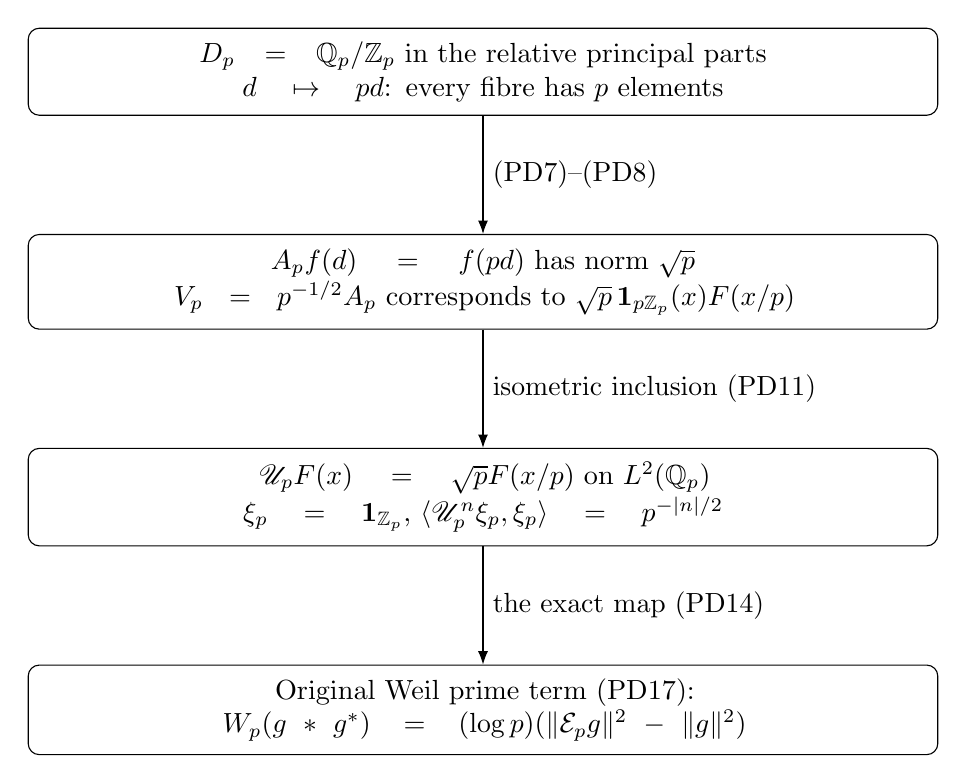
\begin{tikzpicture}[node distance=15mm,
 every node/.style={align=center},
 box/.style={draw,rounded corners,text width=112mm,inner sep=5pt}]
\node[box] (parts) {$D_p=\Q_p/\Z_p$ in the relative principal parts\\
$d\mapsto pd$: every fibre has $p$ elements};
\node[box,below=of parts] (shift) {$A_pf(d)=f(pd)$ has norm $\sqrt p$\\
$V_p=p^{-1/2}A_p$ corresponds to
$\sqrt p\,\mathbf1_{p\Z_p}(x)F(x/p)$};
\node[box,below=of shift] (whole) {$\mathscr U_pF(x)=\sqrt pF(x/p)$ on $L^2(\Q_p)$\\
$\xi_p=\mathbf1_{\Z_p}$,
$\langle \mathscr U_p^n\xi_p,\xi_p\rangle=p^{-|n|/2}$};
\node[box,below=of whole] (energy) {Original Weil prime term (PD17):\\
$W_p(g*g^*)=(\log p)(\|\mathcal E_pg\|^2-\|g\|^2)$};
\draw[-{Latex}] (parts)--node[right]{(PD7)--(PD8)}(shift);
\draw[-{Latex}] (shift)--node[right]{isometric inclusion (PD11)}(whole);
\draw[-{Latex}] (whole)--node[right]{the exact map (PD14)}(energy);
\end{tikzpicture}
\caption{Use of the relative prime data in the original arithmetic pairing.
The prime degree fixes every factor of $p^{1/2}$; the original Haar
measure fixes every norm. Theorems~\ref{thm:PD-dilation} and
\ref{thm:PD-Weil-energy} prove the arrows. The formula retains the
subtracted diagonal energy, both poles and the Archimedean contribution
in (PD18), in the conventions of \cite{Connes1998,Connes2026}.}
\end{figure}

These calculations establish a positive local Hilbert representation
constructed from the relative prime object and the exact signed map
from it into the Weil functional. The full inequality for (PD18) has
not been proved: positivity of each individual squared norm does not
assign the sign of their displayed difference. The new task supplied
by this construction is the full pairing of these relative-prime
operators with the interior and Archimedean objects, with the
subtraction and the two endpoint terms retained.

% END COMPLETE PROOF SOURCE: 13_relative_prime_degree_operator.tex


% BEGIN COMPLETE PROOF SOURCE: 14_all_integers_relative_action.tex
\section{All integers, including supported zero, on the relative object}
\label{sec:all-integers-relative}
The local prime construction extends to the whole relative group
$D=\Q/\Z$. We keep its supported zero $0_D$ and the newly absent
element $\tau_D$ distinct. In particular the integer $e=0_\Z$ is
included in the scalar action, with its exact domain and codomain.

\subsection{Simultaneous arithmetic action and the original integral vector}
For $n\in\Z\setminus\{0\}$ the map $d\mapsto nd$ on $D$ is onto
with kernel $n^{-1}\Z/\Z$, of cardinality $|n|$. Therefore
\[
 (A_nf)(d)=f(nd),\qquad
 \|A_nf\|^2=|n|\|f\|^2,\qquad
 V_n=|n|^{-1/2}A_n
 \tag{IA1}
\]
on $\ell^2(D)$ with counting measure. These formulas follow by counting
each fibre, as in (PD7), and $A_mA_n=A_{mn}$ follows by composition.
The finite character pairings identify $\ell^2(D)$ with
$L^2(\widehat\Z)$, where $\widehat\Z=\prod_p\Z_p$ has Haar measure
one. Indeed every $d=a/N$ gives the character
$x\mapsto\exp(2\pi i a(x\bmod N)/N)$; the finite cyclic
orthogonality proof (PD5) applies with $N$ in place of $p^n$.
The functions factoring through the finite quotients form a dense
subspace, by compactness and the same approximation argument.

Let $\mathbb A_f$ denote the restricted product of the $\Q_p$ with
respect to $\Z_p$, with its original additive Haar measure
$\mu(\widehat\Z)=1$. For a positive rational $a$ define
\[
 (\mathcal U_aF)(x)=\sqrt a\,F(x/a),\qquad F\in L^2(\mathbb A_f).
 \tag{IA2}
\]
The finite-adelic modulus is $|a|_f=a^{-1}$: this follows first for
a prime from $|p|_p=p^{-1}$ and $|p|_q=1$ for $q\ne p$, and then
for all positive rationals by prime factorization. Changing variables
in (IA2) proves unitarity, and composition proves
$\mathcal U_a\mathcal U_b=\mathcal U_{ab}$.
For a positive integer $n$ its restriction to $L^2(\widehat\Z)$ is
the Fourier transform of $V_n$. The proof is the finite character sum
over the kernel of multiplication by $n$: it is zero off
$n\widehat\Z$, and equals $n$ times the original character on that
subgroup. This gives the formula
$\sqrt n\,\mathbf1_{n\widehat\Z}(x)F(x/n)$, including its factor.

Put $\xi=\mathbf1_{\widehat\Z}$, of norm one. For $a=m/n>0$ with
$\gcd(m,n)=1$,
\[
 \langle\mathcal U_a\xi,\xi\rangle=\frac1{\sqrt{mn}}.
 \tag{IA3}
\]
In fact $\widehat\Z\cap a\widehat\Z=m\widehat\Z$, as checked
at each valuation, and its measure is $1/m$. Multiplication by
$\sqrt{m/n}$ proves the displayed equality. In particular, for all
positive integers $m,n$,
\[
 \langle\mathcal U_m\xi,\mathcal U_n\xi\rangle
 =\frac{\gcd(m,n)}{\sqrt{mn}}.
 \tag{IA4}\label{eq:IA-gcd-Gram}
\]
This retains every integral scalar, not only primes or prime powers.
For a finite set of primes the joint scalar spectral measure is exactly
the product of the local measures (PD13): its joint Fourier coefficient
at $(k_p)$ is $\prod_pp^{-|k_p|/2}$ by (IA3). Expanding Laurent
polynomials proves the equality of their pairings with the actual
operators, just as in the proof of (PD13).

The determinant of the matrix (IA4) for $1\le m,n\le N$ is
\[
 \det\left(\frac{\gcd(m,n)}{\sqrt{mn}}\right)_{1\le m,n\le N}
 =\prod_{d=1}^N\frac{\varphi(d)}d>0.
 \tag{IA5}
\]
Here $\varphi(d)$ counts the units of $\Z/d\Z$, with $\varphi(1)=1$.
For completeness, sorting the integers $1,\ldots,k$ by the value of
$\gcd(a,k)$ proves $\sum_{d\mid k}\varphi(d)=k$: those with
$\gcd(a,k)=k/d$ correspond bijectively to residues coprime to $d$.
Thus, for the lower-triangular matrix $E_{md}=\mathbf1_{d\mid m}$,
\[
 (\gcd(m,n))_{m,n}=E\operatorname{diag}(\varphi(1),\ldots,\varphi(N))E^t.
\]
The diagonal of $E$ consists of ones, so its determinant is one.
Taking determinants and retaining the row and column factors
$m^{-1/2},n^{-1/2}$ proves (IA5).
This determinant identity is classical, associated with H. J. S. Smith
\cite{Smith1875}; the complete proof is given here. The calculation
specific to this construction is its realization as the Gram matrix
of the relative-prime operators on the original integral vector.

\subsection{Supported zero acts in an explicitly computed distribution space}
Let $\widetilde D=G(D)=D\sqcup\{\tau_D\}$ with its standard
split-semimodule scalar action. For supported $n\in\Z$,
$n\cdot d=nd$ is supported and $n\cdot\tau_D=\tau_D$.
For the absent scalar $\tau$, every product is $\tau_D$.
Let
\[
 \mathcal T=\C^{(D)}\oplus\C\delta_{\tau_D},\qquad
 \mathcal T'=\C^D\oplus\C,
 \qquad \langle f,h\rangle=\sum_{d\in D}f(d)h(d)+c_f c_h.
 \tag{IA6}
\]
The first factor of $\mathcal T$ consists of finite-support functions,
so the displayed pairing is defined for every $h\in\mathcal T'$.
It is the full algebraic dual pairing. No square-summability condition
is imposed on a distribution in $\mathcal T'$.

Pullback by the scalar maps defines operators $R_a$ on all functions
$\mathcal T'$ satisfying $R_aR_b=R_{ab}$ and $R_1=I$. For nonzero
supported $n$, $R_n$ restricts to (IA1) on $D$ and fixes the absent
coordinate. For the two distinct zeros it gives, exactly,
\[
 R_e(f,c)=(f(0_D)\mathbf1_D,c),\qquad
 R_\tau(f,c)=(c\mathbf1_D,c).
 \tag{IA7}\label{eq:IA-two-zero-operators}
\]
In particular
\[
 R_e\delta_{0_D}=(\mathbf1_D,0),\quad
 R_\tau\delta_{0_D}=0,\quad
 R_e\delta_{\tau_D}=\delta_{\tau_D},\quad
 R_\tau\delta_{\tau_D}=(\mathbf1_D,1).
 \tag{IA8}
\]
Every equality follows by evaluating at a supported $d$ and at
$\tau_D$. They prove, rather than identify away, the difference
between the action of the integer zero and the absent scalar.
Composition of the original scalar maps proves the representation law
also when $a$ or $b$ is either zero. This is a representation of the
\emph{multiplicative scalar monoid}; no false additive identity
$R_{a+b}=R_a+R_b$ is asserted for pullbacks of functions.

There is an exact reason to keep the distribution space (IA6).
The nonzero function $\mathbf1_D$ has infinite counting-measure norm.
Thus $R_e$ has no bounded extension on $\ell^2(D)$ agreeing with
(IA8). Its full action nonetheless exists on $\mathcal T'$ and its
restriction $\mathcal T\to\mathcal T'$ is given by (IA7).
Its Fourier transform on the arithmetic component is
\[
 f(0_D)\mathbf1_D
 \longleftrightarrow
 \left(\int_{\widehat\Z}\mathcal F f(x)\,dx\right)\delta_0.
 \tag{IA9}\label{eq:IA-zero-Fourier}
\]
To prove this without a convergence claim, test against a character
polynomial $F=\sum_da_d\chi_d$. The distribution with all Fourier
coefficients one takes the value $\sum_da_d=F(0)$, which is exactly
$\delta_0$. Orthogonality (PD5) gives
$f(0_D)=\int\mathcal F f$. This proves both sides of (IA9) on every
test. The algebraic transpose of $R_e$ on distributions is also
represented on finite-support tests: it sends
$(f,c)$ to $((\sum_df(d))\delta_{0_D},c)$. Direct substitution in
(IA6) verifies the transpose identity. Thus the mass and supported-zero
evaluation terms are explicit adjoint boundary maps.

The integer $0$ has therefore remained in every scalar map. Its action
lands at a boundary distribution that the Hilbert completion alone
does not contain. The maps (IA7)--(IA9) specify this enlargement and
its relation to the positive Hilbert operators (IA1)--(IA4). Any
purity or duality argument using that Hilbert realization must retain
this computed zero-scalar boundary and its transpose, rather than
quietly delete the integer zero from the programme.

% END COMPLETE PROOF SOURCE: 14_all_integers_relative_action.tex


% BEGIN COMPLETE PROOF SOURCE: 07_original_support_cohomology.tex
\section{Complete support cohomology of the original maps}


The construction starts with the distinct zeros of \(G(R)\) and retains
both of them. It takes finite matrices with their original coefficients
and declared supports to a diagram of cohomology modules over every
compatible support trajectory. This entire diagram carries a canonical
action of \(G_{\LL}(R)\). Its full-support fibre is exactly the original
kernel with its original minimum metric. Nonzero composites are computed
before a sequence is called a complex.

The foundational input is the original semimodule classification
\cite{secondary}, lines 458--945, especially the source labels
\texttt{thm:fiber-modules}, \texttt{thm:reconstruct-semimodule},
\texttt{thm:equivalence-semimodules-diagrams}, and
\texttt{thm:free-semimodule-boolean-cube}.
All reconstruction assertions needed here are proved below.
The original source and conductor matrices are those of OPG5, CEP2--5,
PCL17--21, and GIP1--6 in the pinned source collection \cite{programme}.
No coordinate support is identified across a basis change without its
explicit connecting maps.

\subsection{The two zeros and cancellation paths}

Let \(R\) be a nonzero commutative ring with identity, and let
\[
 S=G(R)=R\sqcup\{\tau\},\qquad e=0_R\in R\subset S.
 \tag{SCD1}
\]
On the supported copy of \(R\), the operations are the ring operations.
The new element \(\tau\) is the additive identity and multiplicative
absorber. Thus \(r+(-r)=e\), not \(\tau\).
The ring projection \(p:S\to R\) sends \(\tau\) to \(0_R\) and fixes
\(R\). The support character \(\chi:S\to\{0,1\}\) sends \(\tau\) to zero
and every supported scalar to one. Checking whether the factors or
summands are supported proves that both are semiring morphisms.
These are the same maps as in the baseline note \cite{globalization}.

For finite sets \(I,J\), a declared support for an \(R\)-matrix
\(d:R^I\to R^J\) is a relation \(D\subseteq J\times I\) containing
every pair with \(d_{ji}\ne0_R\). It may also contain supported zeros.
Define
\[
 \widetilde d_{ji}=
 \begin{cases}d_{ji}\in R\subset S &(j,i)\in D,\\
 \tau &(j,i)\notin D,
 \end{cases}
 \qquad
 D(A)=\{j:\exists i\in A,\ (j,i)\in D\}.
 \tag{SCD2}
\]
The sparse declaration contains exactly the nonzero entries;
the fully entrywise declaration has \(D=J\times I\).
All results below retain whichever support is declared.

A vector of \(S^I\) is a pair \((A,x)\) with \(A\subseteq I\),
\(x\in R^A\). Zero entries of \(x\) are still supported; outside
\(A\) its entries are \(\tau\). Direct matrix multiplication gives
\[
 \widetilde d(A,x)=(D(A),d_{D(A),A}x).
 \tag{SCD3}
\]
Every row with a declared incident edge receives a supported sum,
including a sum that cancels to \(e\).

\begin{proposition}
For \(d:R^I\to R^J\) and \(f:R^J\to R^K\) with supports \(D,F\),
\[
 p(\widetilde f\widetilde d)=fd,\qquad
 \chi(\widetilde f\widetilde d)_{ki}
 =\bigvee_{j\in J}\bigl(\mathbf1_F(k,j)\wedge\mathbf1_D(j,i)\bigr).
 \tag{SCD4}
\]
If \(fd=0_R\), the lifted composite has entry \(e\) at every
declared length-two path and \(\tau\) elsewhere. It is the global
zero matrix over \(S\) exactly when there are no such paths.
\end{proposition}
\begin{proof}
A product in the sum is supported exactly when both entries are
supported. Its ring value is \(f_{kj}d_{ji}\), even when that product
is zero. A nonempty sum of supported terms is supported and has the
ring sum as its value. Only an empty supported sum is \(\tau\).
This proves every assertion, including rings with zero divisors.
The cancellation certificate \(\sum_j f_{kj}d_{ji}=0_R\) therefore
retains all of its individual paths.
\end{proof}

In particular,
\[
 d_0=\begin{pmatrix}1\\1\end{pmatrix},\qquad
 d_1=\begin{pmatrix}1&-1\end{pmatrix},
 \qquad d_1d_0=0_R,\quad \widetilde d_1\widetilde d_0=(e).
 \tag{SCD5}
\]
The exact morphism \(p\) carries this \(e\) to \(0_R\).
It does not identify \(e\) and \(\tau\) in \(S\).

\subsection{Every compatible support trajectory}

Fix a finite cochain complex with its original based matrices:
\[
 C^n=R^{I_n},\quad d_n:C^n\to C^{n+1},\quad
 d_{n+1}d_n=0_R.
 \tag{SCD6}
\]
Only finitely many \(I_n\) are nonempty. Fix every declared support \(D_n\).
A support trajectory is a sequence \(A=(A_n)_n\), \(A_n\subseteq I_n\),
with \(D_n(A_n)\subseteq A_{n+1}\). Let \(\LL_D\) be their componentwise
ordered set.

\begin{theorem}
The lattice \(\LL_D\) is complete and distributive. Its meet and join
are componentwise intersection and union, its bottom is the empty
trajectory, and its top is \(\mathbf I=(I_n)_n\).
For arbitrary seed sets \(U_n\subseteq I_n\), their smallest containing
trajectory is
\[
 \cl_D(U)_n=U_n\cup
 \bigcup_{m<n}D_{n-1}\cdots D_m(U_m).
 \tag{SCD7}
\]
This closure is monotone, idempotent, and preserves unions.
\end{theorem}
\begin{proof}
An edge starting in a union starts in one member, whose next component
contains its endpoint. An edge starting in an intersection has its
endpoint in every next component. Thus arbitrary unions and intersections
are trajectories, with the stated empty conventions. Set-theoretic
distributivity proves the lattice assertion. Every path endpoint in SCD7
is forced in any containing trajectory. Appending one edge proves that
SCD7 itself is a trajectory. This proves minimality and all closure laws.
\end{proof}

Equivalently the graded vertices \((n,i)\) carry directed edges
\((n,i)\to(n+1,j)\) from \(D_n\). Degrees strictly increase, so
reachability defines a finite partial order. The trajectories are
exactly its upward-closed subsets. Every path remains visible.

\begin{theorem}
For \(A\in\LL_D\) put
\[
 C_A^n=R^{A_n},\qquad d_{n,A}=(d_n)_{A_{n+1},A_n}.
 \tag{SCD8}
\]
These are cochain complexes. Extension by zero \(j_{AB}^n:C_A^n\to C_B^n\)
for \(A\subseteq B\) is an injective cochain map. Consequently
\[
 Z_A^n=\ker d_{n,A},\quad B_A^n=\im d_{n-1,A},\quad
 H_A^n=Z_A^n/B_A^n,\qquad
 h_{AB}^n[x]=[j_{AB}^nx]
 \tag{SCD9}
\]
defines a diagram of \(R\)-modules, with exact composition of its maps.
\end{theorem}
\begin{proof}
If \(i\in A_n\) and \(d_{n,ji}\ne0\), then \(j\in A_{n+1}\).
Thus the restricted intermediate sum removes no nonzero term:
\[
 (d_{n+1,A}d_{n,A})_{ki}
 =\sum_{j\in I_{n+1}}d_{n+1,kj}d_{n,ji}=0_R.
\]
Every declared intermediate path is also included in \(A_{n+1}\),
so its cancellation is retained. The same support condition says
that applying \(d_n\) to a vector supported in \(A_n\) produces
a vector in \(R^{A_{n+1}}\). Therefore extension by zero commutes
with the differential. It maps cycles and boundaries to cycles
and boundaries; this proves the quotient map is well defined.
Linearity, identity, and composition follow from zero extension.
\end{proof}

For \(A\subseteq B\), identify the smaller coordinate modules with
their zero-extended copies. The exact kernels and cokernels are
\[
 \ker h_{AB}^n=(Z_A^n\cap B_B^n)/B_A^n,\qquad
 \operatorname{coker}h_{AB}^n=Z_B^n/(Z_A^n+B_B^n).
 \tag{SCD10}
\]
Indeed a smaller cycle becomes zero precisely when it becomes a
larger boundary, and the image is
\((Z_A^n+B_B^n)/B_B^n\).
For SCD5 there are exactly six trajectories: the empty one; the
last vertex; either middle vertex with the last; both middle vertices
with the last; and the full set. The penultimate one has
\(H^1=R(1,1)\), which becomes a boundary in the full exact complex.
The last-vertex fibre has \(H^2=R\). Thus exactness at full support
does not discard the nontrivial cohomology at smaller supports.

\subsection{Reconstruction and the full \(G_{\LL_D}(R)\) base}

Define the disjoint union, retaining its index even when a module is zero,
\[
 \mathcal H_D^n=\bigsqcup_{A\in\LL_D}H_A^n.
 \tag{SCD11}
\]
For elements in two fibres use
\[
 (A,[x])+(B,[y])
 =\bigl(A\cup B,\ h_{A,A\cup B}[x]+h_{B,A\cup B}[y]\bigr).
 \tag{SCD12}
\]
A supported \(r\in R\) acts within its fibre, and \(\tau\) acts by
the bottom-fibre zero. Define \(\mathcal C_D^n,\mathcal Z_D^n,
\mathcal B_D^n\) from \(C_A^n,Z_A^n,B_A^n\) in the same way.

\begin{theorem}
These operations make \(\mathcal H_D^n\) a \(G(R)\)-semimodule.
Its support lattice is exactly \(\LL_D\), its fibres are exactly
\(H_A^n\), and its transports are \(h_{AB}^n\). It is the quotient
of \(\mathcal Z_D^n\) by the congruence
\[
 (A,x)\sim(B,y)
 \quad\Longleftrightarrow\quad A=B\ \hbox{ and }\ x-y\in B_A^n.
 \tag{SCD13}
\]
Thus different support indices are never identified.
\end{theorem}
\begin{proof}
Three summands may all be transported to \(A\cup B\cup C\).
Functoriality of \(h\) makes either parenthesization equal to
the same sum in that module. Commutativity and the bottom identity
follow in the same way. Linearity of transport proves both scalar
distributive laws. In particular \((r+s)x=rx+sx\) occurs in the
same fibre, also when \(r+s=0_R\). The rules involving \(\tau\)
follow from its action. The supported zero acts by
\(e(A,[x])=(A,0)\), and
\((A,0)+(B,0)=(A\cup B,0)\), identifying the support lattice.
Boundaries transport to boundaries, so SCD13 is preserved under
addition and scalars. Its fibre quotient is precisely \(H_A^n\).
\end{proof}

There is an exact distinction between this construction and a
falsely asserted global square-zero lift. Put
\[
 \mathcal D_n(A,x)=(A,d_{n,A}x),\qquad
 \mathbf z_{n,n+2}(A,x)=(A,0).
 \tag{SCD14}
\]
They are \(S\)-linear and
\(\mathcal D_{n+1}\mathcal D_n=\mathbf z_{n,n+2}\).
For nontrivial \(\LL_D\), this is not the global zero map,
whose output has index \(\varnothing\). The usual preimage of
that global zero is not the union of fibre kernels.
Cohomology is taken in the additive category of \(R\)-module
diagrams on the fixed lattice, as explicitly specified in SCD9,
then reconstructed by SCD11--13.

The exact return map to the original free semimodule is
\[
 E_n:\mathcal C_D^n\to S^{I_n},\qquad E_n(A,x)=(A_n,x).
 \tag{SCD15}
\]
It is \(S\)-linear because supports of sums are unions and
zero extensions commute with addition. It can fail to be injective:
two distinct trajectories may have the same \(n\)-th support.
The original lifted matrix is related to it by
\[
 E_{n+1}\mathcal D_n(A,x)
 =T_{D_n(A_n),A_{n+1}}\bigl(\widetilde d_n E_n(A,x)\bigr).
 \tag{SCD16}
\]
Here \(T\) inserts supported zeros at the additional coordinates,
exactly as in the Boolean-cube diagram of \(S^{I_{n+1}}\).
SCD3 and SCD8 prove this identity at every coordinate.

We now include all support scalars. For the bounded distributive
lattice \(\LL=\LL_D\), define
\[
 G_{\LL}(R)
 =\{(r,\mathbf I):r\in R\}\ \cup\
   \{z_A=(0_R,A):A\in\LL\}\ \subset R\times\LL,
 \tag{SCD17}
\]
with coordinatewise operations
\[
 (r,A)+(s,B)=(r+s,A\cup B),\qquad
 (r,A)(s,B)=(rs,A\cap B).
\]
It is a subsemiring of the product of the ring \(R\) and the lattice
semiring \((\LL,\cup,\cap)\): closure follows because a nonzero
ring coordinate requires full support. The zero is \(z_\varnothing\),
the unit is \((1,\mathbf I)\), and
\((0_R,\mathbf I)=z_{\mathbf I}\) is the supported \(e\).

\begin{theorem}[Canonical action of every support scalar]
Every module diagram on \(\LL\), and in particular the cochain,
cycle, boundary and cohomology diagrams above, has the action
\[
 (r,\mathbf I)(A,x)=(A,rx),\qquad
 z_\lambda(A,x)=(\lambda\cap A,0).
 \tag{SCD18}
\]
This defines a \(G_{\LL}(R)\)-semimodule. Restricting along
\[
 G(R)\longrightarrow G_{\LL}(R),\qquad
 \tau\longmapsto z_\varnothing,\quad
 r\longmapsto(r,\mathbf I)
 \tag{SCD19}
\]
recovers exactly the preceding \(G(R)\)-semimodule.
The scalar map is injective whenever \(\varnothing\ne\mathbf I\).
\end{theorem}
\begin{proof}
The two rules agree at the shared element
\((0_R,\mathbf I)=z_{\mathbf I}\): both give \((A,0)\).
A supported scalar preserves the label and acts linearly. For a
zero-support scalar, additivity on vectors is exactly
\[
 \lambda\cap(A\cup B)=(\lambda\cap A)\cup(\lambda\cap B),
\]
because linear transport sends a zero to a zero. Scalar addition
of two such elements uses the other distributive identity,
\((\lambda\cup\mu)\cap A=(\lambda\cap A)\cup(\mu\cap A)\).
If one scalar is \((r,\mathbf I)\) and the other is \(z_\lambda\),
their sum is \((r,\mathbf I)\); the vector sum is
\((A,rx)+(\lambda\cap A,0)=(A,rx)\), as required.
For two supported scalars, scalar additivity is the ordinary
module law, even if their sum is the supported zero.

For scalar multiplication, two zero-support scalars give
\((\lambda\cap\mu)\cap A\). A supported scalar followed or preceded
by \(z_\lambda\) gives the same zero in \(\lambda\cap A\).
Two supported scalars satisfy the ordinary module multiplication
law, also when their product is zero in \(R\).
The unit acts as identity. The global zero maps to the zero of
the bottom fibre, hence is the required absorber. All semimodule
axioms have now been checked. The homomorphism SCD19 follows
directly from SCD17, and its restriction gives the declared action
of both \(\tau\) and every supported scalar. Injectivity follows
from the distinct support coordinates.
\end{proof}

The maps in SCD14 and the cohomology quotient are linear for this
larger semiring: each takes the zero in a fibre to the zero in the
same fibre. Coordinate extraction SCD15 is equivariant along the
scalar morphism
\[
 G_{\LL}(R)\to G_{\mathcal P(I_n)}(R),\qquad
 (r,\mathbf I)\mapsto(r,I_n),\quad z_A\mapsto z_{A_n},
\]
because the coordinate map \(A\mapsto A_n\) preserves union,
intersection, bottom and top.

\begin{theorem}[Exact additive group completion and arithmetic receiver]
The map
\[
 \epsilon_{\rm full}:\mathcal H_D^n\to H_{\mathbf I}^n,\qquad
 (A,[x])\longmapsto h_{A,\mathbf I}^n[x]
 \tag{SCD20}
\]
is the universal additive group completion. It is also the universal
linear map to an \(R\)-module, for the scalar projection
\(\pi:G_{\LL}(R)\to R,\ (r,A)\mapsto r\).
Thus the original cohomology is recovered exactly on the arithmetic
quotient \(G_{\LL}(R)/(e)\cong R\), while every other fibre remains
in \(\mathcal H_D^n\).
\end{theorem}
\begin{proof}
The displayed map preserves addition and is onto, using the top
fibre. Any additive map from \(\mathcal H_D^n\) to an abelian group
kills every \((A,0)\), since it is additively idempotent and the
target permits cancellation. But
\[
 (A,[x])+(\mathbf I,0)
 =(\mathbf I,h_{A,\mathbf I}[x]).
\]
Applying the map forces its value on \((A,[x])\) to be its value
on that transported top-fibre element. The restriction to the
top fibre is a group homomorphism. This proves unique factorization
through SCD20 for every abelian target, hence the universal
group-completion assertion. For \(R\)-linear targets the same proof
retains scalar linearity.

The scalar projection is a semiring morphism. Its kernel ideal
is the full zero-amplitude fibre \(\{z_A:A\in\LL\}\), which equals
the principal ideal \((e)\): \(ez_A=z_A\), while multiplying \(e\)
by any scalar and adding such products always has zero amplitude.
Moreover addition by \(e=z_{\mathbf I}\) sends every zero-amplitude
scalar to \(e\). The congruence identifying \(e\) with the global
zero therefore identifies every \(z_A\) with zero, and leaves
exactly the ring operations on \(R\). Conversely \(\pi\) separates
all different ring amplitudes. Thus this quotient is exactly \(R\).
Finally SCD20 sends \(z_\lambda(A,[x])\), a fibre zero, to zero
and sends supported scalars to their usual action, proving its
\(\pi\)-linearity.
\end{proof}

\subsection{Gluing, matrix changes, and the space defined by curvature}

For \(A,B\in\LL_D\), the original coordinate inclusions give
a degreewise exact sequence of complexes
\[
 0\to C_{A\cap B}\xrightarrow{x\mapsto(x,-x)}
 C_A\oplus C_B\xrightarrow{(x,y)\mapsto x+y}C_{A\cup B}\to0 .
 \tag{SCD21}
\]
Surjectivity follows by assigning coordinates in \(A\) to the first
summand and those in \(B\setminus A\) to the second. A pair summing
to zero has equal and opposite entries supported in the intersection,
which proves exactness. SCD8 proves compatibility with the differentials.

If \(z\) is a cycle in the union, choose \(z=x+y\) in the two
summands. Then \(d_Ax=-d_By=w\) is an intersection cycle. Set
\[
 \partial[z]=[w],\qquad
 \cdots\to H_{A\cap B}^n\to H_A^n\oplus H_B^n
 \to H_{A\cup B}^n\xrightarrow{\partial}H_{A\cap B}^{n+1}\to\cdots .
 \tag{SCD22}
\]
A new splitting changes \((x,y)\) by \((t,-t)\) with \(t\) in
the intersection, so \(w\) changes by \(dt\). Splitting a primitive
of a boundary shows independence of the representative of \([z]\).
For exactness at the middle term, if a pair of cycles sums to a
boundary, subtract a split primitive to make its sum zero. It then
comes from an intersection cycle. If \(\partial[z]=0\), subtract
an intersection primitive from one splitting term and add it to
the other; both become cycles, proving exactness at the union.
Finally if an intersection cycle maps to boundaries in both larger
spaces, choose primitives with opposite signs. Their sum is a union
cycle mapping to that intersection class. These arguments verify
all three repeating positions and also that each composite is zero.

For an actual cochain map \(F_n:C^n\to C'{}^n\), let \(P_n\)
be a declared support containing its nonzero coefficients, and
let \(D'\) be the target differential supports. Then
\[
 F_\#A=\cl_{D'}((P_n(A_n))_n)
 \tag{SCD23}
\]
preserves joins and bottom, and the same matrices restrict to
cochain maps \(C_A\to C'_{F_\#A}\). This follows from \(d'F=Fd\)
and the defining support closure; hence it induces cohomology maps.
If \(G\) is another map with declared supports \(Q_n\), and the
declared support of \(GF\) is contained in \(Q_nP_n\) while retaining
every nonzero coefficient, then
\[
 (GF)_\#A\subseteq G_\#F_\#A .
 \tag{SCD24}
\]
Indeed the trajectory on the right contains every composite
coordinate before cancellation. Its minimal closed subtrajectory
contains the direct product support. The composite cohomology map
equals the direct one followed by this inclusion, since their
underlying matrices are equal. This is the exact comparison when
a cancellation changes the minimal support. An invertible basis
change gives an isomorphism at full support; it is not asserted
to give a bijection of coordinate support lattices.

The reconstructed map is always \(G(R)\)-linear. Its exact
compatibility with the additional lattice scalars is the transport
of a zero along
\[
 F_\#(\lambda\cap A)\subseteq F_\#\lambda\cap F_\#A.
\]
The left side is the support of the image of \(z_\lambda(A,x)\);
the right side is the support obtained by applying
\(z_{F_\#\lambda}\) to the image of \((A,x)\). Both amplitudes
are zero, and the stated inclusion gives their exact diagram map.
It follows from monotonicity of \(F_\#\). If \(F_\#\) also
preserves intersections and top, it induces a semiring morphism
on the two \(G_{\LL}(R)\) bases, and this comparison is equality.
Thus an arbitrary matrix change has the proved support transport,
without an unproved scalar-base isomorphism.

Now allow arbitrary consecutive matrices with
\[
 \Omega_n=d_{n+1}d_n
 \tag{SCD25}
\]
possibly nonzero, and retain the same trajectory lattice.
For a trajectory \(A\), the restricted composite is exactly
\((\Omega_n)_{A_{n+2},A_n}\), by the intermediate-index proof of
SCD8. Define the forbidden vertices to be those \((n,i)\)
whose \(i\)-th column in \(\Omega_n\) is not the zero vector.
Include all ancestors of these vertices in the forbidden set,
and let \(T\) be its complement.

\begin{theorem}[The curvature defines a maximal exact support space]
The set \(T\) is a trajectory. The trajectories whose restricted
matrices are complexes are exactly
\[
 \{A\in\LL_D:A\subseteq T\}.
 \tag{SCD26}
\]
They form a complete distributive lattice with top \(T\).
\end{theorem}
\begin{proof}
An edge from a non-forbidden vertex cannot reach a forbidden
vertex, since that would make its starting vertex an ancestor
of a forbidden vertex. Hence \(T\) is forward closed.
If column \(i\) of \(\Omega_n\) is nonzero, choose \(k\)
with \((\Omega_n)_{ki}\ne0\). At least one summand
\(d_{n+1,kj}d_{n,ji}\) is nonzero, so there is a declared path
from \((n,i)\) to \((n+2,k)\). Every trajectory containing
the first contains the last, and its restricted curvature
therefore has that nonzero entry. It cannot be a complex.
It also cannot contain an ancestor of the first vertex.
Conversely, a trajectory contained in \(T\) contains no initial
column on which \(\Omega_n\) is nonzero. All restricted composites
are therefore zero. Closure under unions and intersections and
the top assertion follow directly.
\end{proof}

This retains the full original curvature rather than declaring it zero.
There is also an exact correction using submodules beyond coordinate
supports. For consecutive maps \(d,f\),
\[
 d(\ker(fd))=\im d\cap\ker f .
 \tag{SCD27}
\]
Both inclusions follow from \(f(dx)=0\). Restricting the first
domain to \(\ker(fd)\) gives a genuine complex, while retaining
the explicit defect \(fd\) and the exact connecting inclusion.
Thus the obstruction specifies both a coordinate-support lattice
and its potentially larger linear submodule receiver.

\subsection{The original source, conductor and invariant observation}

At every literal original cutoff retain
\[
 N\in\{q-1,q,2q-1,2q\},\qquad
 \Pp_N=\C[S]_{\le N},\qquad E=\C[S]/(\chi_k),
 \quad U_N:\Pp_N\to E,\quad p\mapsto[p].
 \tag{SCD28}
\]
The polynomial \(\chi_k\) is the complete original monic root
polynomial of degree \(q\). The source inner product is the original
one, with its complete mass. Polynomial and primary coordinates
are connected by the actual Vandermonde matrix.

The observation is exactly the original OPG5 map:
\[
 P_k=\frac1{n+1}\sum_{a=0}^{n}(C^{-a})^{\otimes k},\qquad
 L=P_k\Pi^{\otimes k}U^{\otimes k}\iota,\qquad
 B=\im L,\quad\jmath\Lambda=L,\quad K=\ker\Lambda .
 \tag{SCD29}
\]
The \(U\) in this tensor formula is the original period-unit map,
distinct from the remainder \(U_N\). Every original period and
invariant column in \(P_k,\Pi,U,\iota\) is kept. See the exact
\href{https://github.com/KokunoYumeto/zeta-function-research-reader/blob/6cf5b3aa8ff395eba6b5512b28d117334da5767b/workbenches/splitzero-tandem/continuations/20260922-cutoff-profile/RETAINED_COMPLETE_PROOF_SOURCES.tex#L9420}{OPG4--5 definition and original cycle action}.

Let \(Z_{\chi,N}\) be multiplication by the complete \(\chi=\chi_k\),
including its conversion to the original source coordinates.
Use \(\Pp_{N-q}=0\) when \(N=q-1\). Then
\[
 \Pp_{N-q}\xrightarrow{Z_{\chi,N}}\Pp_N
                  \xrightarrow{\Lambda U_N}B
 \tag{SCD30}
\]
is a complex, with degrees zero, one and two. Its cohomology is
\[
 H^0=0,\qquad
 H^1\xrightarrow{\sim}K,\quad[p]\mapsto U_Np,\qquad H^2=0.
 \tag{SCD31}
\]
Multiplication by a monic nonzero polynomial is injective.
Division by \(\chi\) proves
\(\ker U_N=\chi\Pp_{N-q}\); \(U_N\) is onto since \(N\ge q-1\).
A cycle therefore maps to \(K\), every member of \(K\) has a lift,
and two lifts differ by exactly a relation. The map to \(B\)
is onto, proving the last assertion. Applying SCD7--20 to these
complete matrices supplies the full \(G_{\LL_D}(\C)\)-cohomology
object, with precisely \(K\) as its terminal arithmetic fibre.

For the conductor graph, retain its original simple-quartet domain
\(m=1,\ k=4l+1\ge9,\ q=(k+1)^2,\ q'=(k-7)^2\).
No conclusion about a more general multiplicity is imported from
this graph presentation. Retain all coefficients of
\(A=\sum_{a,b=0}^8a_{ab}e_{ab}^{(8)}\), all its shifts \(b_{ab}\),
and the original lower polynomial \(\chi'=\chi_{k-8}\). The prime
in \(\chi'\) denotes that polynomial, not a derivative. The maps are
\[
 (\mathcal T_Ap)(S')=\sum_{a,b=0}^8a_{ab}p(S'+b_{ab}),\qquad
 C_{(i,j),(u,w)}=
 \begin{cases}a_{u-i,w-j}&0\le u-i,w-j\le8,\\
 0&\text{otherwise}.
 \end{cases}
 \tag{SCD32}
\]
The root identity \(\beta'_{ij}+b_{ab}=\beta_{i+a,j+b}\)
gives \(\chi'\mid\mathcal T_A(\chi h)\) for every \(h\).
Thus \(\mathcal T_A\) induces the map on quotient spaces with
matrix \(V_{\beta'}^{-1}CV_\beta\). The transpose \(C^{\mathsf T}\)
is multiplication by the nonzero biform \(A\), hence injective
in the polynomial domain. Therefore \(C\) is onto. Its kernel
\(V_A\subset E\) contains the actual \(K\), by OCF17 and CEP5.

The complete pivot and remaining invariant-image maps are retained:
\[
 CN_k^{\mathsf T}=0,\quad
 S_k^{\mathsf T}N_k^{\mathsf T}=I,\quad
 \im N_k^{\mathsf T}=V_A,\qquad J_R=S_kZ_k .
 \tag{SCD33}
\]
These identities hold in the original primary coordinates.
Here \(Z_k\) contains all additional invariant columns, so after
imposing the conductor equation the complete residual equations
still include \(J_R^{\mathsf T}V_\beta p=0\), as in CG29.
The actual residual observation is
\[
 \Xi=\Lambda|_{V_A}:V_A\to B_A=\Lambda(V_A),\qquad\ker\Xi=K.
\]
In the original fixed residual frame it is \(\Xi_k^{\rm fix}\);
changing to that frame retains its full invertible target map.
No formula below substitutes a historical rank numeral for
\(\dim K\) or \(\dim B_A\).

Let \(v\) be the first nonzero translation moment order. The actual
invertible source map \(S_N\) takes a polynomial to its first \(v\)
original source coordinates and its \(\mathcal T_A\) image.
To see invertibility, Taylor's finite expansion says
\(\mathcal T_A\) lowers each degree at least \(v\) by exactly \(v\)
and kills exactly \(\Pp_{v-1}\). The first \(v\) source coordinates
are an isomorphism on that kernel. The source and target dimensions
are equal, so the displayed injective map is invertible.
Define the original graph maps
\[
 \begin{gathered}
 X_N=\C^v\oplus\C[S']_{\le N-v-q'},\qquad
 D_N=\operatorname{diag}(I_v,M_{\chi'}),\\
 E_N=U_NS_N^{-1}D_N:X_N\to V_A,\qquad
 B_N=\Xi E_N:X_N\to B_A .
 \end{gathered}
 \tag{SCD34}
\]
Here \(D_N\) includes the exact conversion to the lower original
source coordinates. The equality
\(S_N^{-1}D_NX_N=U_N^{-1}(V_A)\) follows from divisibility by
\(\chi'\). Consequently \(E_N\) is onto \(V_A\).

The full original relation columns are
\[
 \begin{gathered}
 \mathcal Z_Nh=
 \begin{pmatrix}P_{<v}Z_{\chi,N}h\\\mathcal U_{A,N-q}h\end{pmatrix},
 \qquad D_N\mathcal Z_N=S_NZ_{\chi,N},\\
 (\mathcal U_{A,N-q}h)(S')
 =\sum_{a,b=0}^8a_{ab}d_{ab}(S')h(S'+b_{ab}),\qquad
 d_{ab}(S')=\chi(S'+b_{ab})/\chi'(S').
 \end{gathered}
 \tag{SCD35}
\]
Each \(d_{ab}\) is the original complete product of root differences.
Multiplication by \(\chi'\) proves the lower equality using SCD32;
the upper block is exactly the retained lower source coordinates.
Thus \(\mathcal Z_N\) is injective and
\(\ker E_N=\im\mathcal Z_N\).

The correct graph complex and its full-support cohomology are
\[
 \Pp_{N-q}\xrightarrow{\mathcal Z_N}X_N\xrightarrow{B_N}B_A,
 \qquad H^1\xrightarrow{\sim}K,\quad[x]\mapsto E_Nx,
 \qquad H^0=H^2=0 .
 \tag{SCD36}
\]
Injectivity, surjectivity and \(\ker\Xi=K\) prove these statements
exactly as in SCD31. The chain map to SCD30 is
\[
 (I,\ S_N^{-1}D_N,\ B_A\hookrightarrow B).
 \tag{SCD37}
\]
Its squares are SCD35 and
\(\Lambda U_NS_N^{-1}D_N=\Xi E_N\). Its induced middle
cohomology map is the identity of \(K\). On support trajectories
the exact map is SCD23 with the actual coefficient supports of
these three maps. Hence the support comparison is proved as well.

Choose the full original kernel frame \(I_K\) with actual rank
\(r=\dim K\). In original orthonormal source coordinates let
\(G_N=(U_NU_N^*)^{-1}\), and set
\[
 W_{K,N}=D_N^{-1}S_NU_N^*G_NI_K,\qquad
 E_NW_{K,N}=I_K .
\]
The inverse of \(D_N\) is used only on its indicated image;
the minimum lift is in \(U_N^{-1}(V_A)\). Then the exact kernel is
\[
 \ker B_N=\im[\mathcal Z_N,W_{K,N}],\qquad
 \rk[\mathcal Z_N,W_{K,N}]=(N-q+1)+r .
 \tag{SCD38}
\]
Applying \(E_N\) to a relation among those columns first kills
the coefficients of the independent \(I_K\). Injectivity of
\(\mathcal Z_N\) then kills the remainder. Conversely subtract
the corresponding \(W_{K,N}\) lift from any vector in \(\ker B_N\);
what remains lies in \(\ker E_N\). This proves every column and
rank assertion, including the empty relation list at \(N=q-1\).

The longer sequence \(X_N\xrightarrow{E_N}V_A\xrightarrow{\Xi}B_A\)
has the exact curvature
\[
 \Xi E_N=B_N:X_N\twoheadrightarrow B_A .
 \tag{SCD39}
\]
It is a complex only when the actual \(B_A\) is zero. In all cases
its zero-curvature submodule is precisely SCD38. Thus the nonzero
defect of that proposed sequence is retained, while SCD36 gives
the genuine original graph complex.

\subsection{Exact return to the original metric and arithmetic action}

The full-support identification preserves the actual minimum metric.
For a fixed \(x\in K\), all representatives in SCD30 differ by
\(\chi h\). Minimizing their complete source norm is precisely
the definition of the original quotient norm on \(E\). Thus in
the unchanged full kernel frame it is
\[
 H^K_N=I_K^*G_NI_K .
 \tag{SCD40}
\]
For the graph complex, its actual source metric is
\[
 H_N^{\rm actual}=D_N^*S_N^{-*}S_N^{-1}D_N .
 \tag{SCD41}
\]
The map \(S_N^{-1}D_N\) in SCD37 is then an isometry onto its
image. Every representative of \(x\in K\) lies in
\(U_N^{-1}(V_A)\), so the same minimum gives exactly SCD40.
This proof does not substitute the alternative graph product
metric \(D_N^*D_N\) for SCD41. For all four cutoffs, the full
cohomology determinant is therefore the original determinant,
including the original signed return
\[
 \begin{split}
 &\log\det H^{\rm coh}_{q-1,\mathbf I}
 +\log\det H^{\rm coh}_{q,\mathbf I}
 -\log\det H^{\rm coh}_{2q-1,\mathbf I}
 -\log\det H^{\rm coh}_{2q,\mathbf I}\\
 &\hspace{8mm}=
 \log\det H^K_{q-1}+\log\det H^K_q
 -\log\det H^K_{2q-1}-\log\det H^K_{2q}.
 \end{split}
 \tag{SCD42}
\]
Use the same \(I_K\) at every endpoint and the original empty
determinant convention. This exact identity assigns no missing
asymptotic coefficient.

The original multiplication \(M:E\to E\) need not preserve \(K\).
Its failure to descend through observation is explicitly computable.
Keep the full minimum section and observed action
\[
 Q_N=(\Lambda G_N^{-1}\Lambda^*)^{-1},\quad
 L_N=G_N^{-1}\Lambda^*Q_N,\quad P_N=L_N\Lambda,\quad
 M_{B,N}=\Lambda ML_N .
\]
Then
\[
 \Lambda M-M_{B,N}\Lambda
 =\Lambda M(I-P_N)
 =\Lambda MI_K(H_N^K)^{-1}I_K^*G_N .
 \tag{SCD43}
\]
For proof, direct multiplication gives the first equality.
The minimum section is orthogonal to \(\ker\Lambda=K\);
hence \(I-P_N\) is the \(G_N\)-orthogonal projector onto \(K\).
The displayed expression \(I_K(H_N^K)^{-1}I_K^*G_N\)
is the same projector: multiply to verify idempotence, image,
identity on \(K\), and weighted self-adjointness. This proves
the final equality without deleting its kernel block.

The exact action-compatible subspace and defect space are
\[
 0\to K\cap M^{-1}K\to K
 \xrightarrow{\Lambda M}\im(\Lambda M|_K)\to0.
 \tag{SCD44}
\]
The kernel assertion is its definition; the last target is the
actual image. Thus this is the exact obstruction to obtaining
an action on the original middle cohomology by \(M\).

Retain every higher observation as well:
\[
 K^{(j)}=\bigcap_{a=0}^{j}\ker(\Lambda M^a),\qquad j\ge0.
 \tag{SCD45}
\]
The connecting maps are inclusions, and
\(K^{(j+1)}=K\cap M^{-1}K^{(j)}\). If two successive spaces
are equal, the common space is \(M\)-invariant: membership in
\(K^{(j+1)}\) implies that the \(M\)-image belongs to \(K^{(j)}\).
It is then killed by every further observation, so the sequence
stabilizes. It has at most \(\dim K\) strict drops. Its stable
value is the largest \(M\)-invariant subspace of \(K\), since
every such subspace is killed by every \(\Lambda M^a\), while
the stable value itself is invariant. This is a specified space
with exact connecting maps, rather than an assumed descent.

The original metrics, periods and roots are unchanged throughout.
The construction provides a complete support object over the
absolute base, its exact arithmetic receiver, and the spaces
defined by the two original curvature defects SCD39 and SCD43.
No support trajectory or additional invariant column is discarded.

\subsection{One support base for the four original cutoffs}

The four support bases need not be identified by choosing bases again.
There is a single exact common construction. For a fixed original source
order \(s\in\{1,k\}\), retain the original source inclusions
\(i_{NM}:\Pp_N\hookrightarrow\Pp_M\), \(N<M\), at the four cutoffs.
On relation polynomials use \(j_{NM}:\Pp_{N-q}\hookrightarrow\Pp_{M-q}\)
and on \(B\) use the identity. Their original matrices satisfy
\[
 i_{NM}Z_{\chi,N}=Z_{\chi,M}j_{NM},\qquad
 U_Mi_{NM}=U_N,\qquad
 \Lambda U_Mi_{NM}=\Lambda U_N .
 \tag{SCD46}
\]
These are identities on polynomials before passing to any coordinates.
Their matrices include whatever original basis conversions are required.
They form cochain maps of SCD30 and induce precisely the identity of
\(K\) in SCD31.

For the graph presentations, the corresponding map is
\[
 F^X_{NM}=D_M^{-1}S_Mi_{NM}S_N^{-1}D_N,\qquad
 E_MF^X_{NM}=E_N,\quad
 F^X_{NM}\mathcal Z_N=\mathcal Z_Mj_{NM}.
 \tag{SCD47}
\]
The inverse of \(D_M\) is taken only on its actual image: a polynomial
whose class lies in \(V_A\) still has that property after source inclusion,
so \(S_M\) of that polynomial has its second component divisible by
\(\chi'\). This proves that the map is defined. Cancellation of the
displayed inverse maps, followed by SCD35 and SCD46, proves the two
identities. Composition for three source cutoffs follows by the same
cancellation. The induced cohomology map is again the identity of \(K\).

Now form a finite coefficient graph whose vertices record the cutoff,
cochain degree and coefficient index. Include every declared differential
edge, every edge of these original horizontal source maps, and, if both
presentations are retained together, every edge of the graph-to-polynomial
map SCD37. Let \(\LL_{\rm all}\) be all subsets closed under these edges.
One can include both source orders as separately labelled copies, without
identifying their metrics. The proof of SCD7 applies to this finite
diagram: unions and intersections remain closed, and forward closure is
the least containing closed set. Thus \(\LL_{\rm all}\) is a finite bounded
distributive lattice with all the original coefficient supports retained.

The coordinate projection to any one of the complexes preserves union,
intersection, bottom and top, and takes a master trajectory to a valid
local trajectory. Restricting every original matrix at a master trajectory
therefore gives a diagram of complexes in which all original squares
still commute. To verify a square entry, note that every intermediate
index with a nonzero contribution is forced into the master trajectory
by its first edge; its second edge is retained as well. Thus the restricted
entry is the original full entry, with all its cancellation terms.

For each cutoff reconstruct
\[
 \mathcal H_{\rm all,N}^1
 =\bigsqcup_{A\in\LL_{\rm all}}H^1_{N,A|_N}.
 \tag{SCD48}
\]
These are modules over the \emph{same} \(G_{\LL_{\rm all}}(\C)\) by
SCD18. The horizontal cohomology maps preserve the master label \(A\),
commute with union transports, and take a zero in a fibre to the zero in
the same fibre. They are therefore \(G_{\LL_{\rm all}}(\C)\)-linear:
for \(z_\lambda\) both composites give the zero at \(\lambda\cap A\);
for a supported scalar the assertion is ordinary linearity.
Their additive group completions all equal the same \(K\), with identity
connecting maps and the four separate original metrics SCD40.
This proves a common absolute-base receiver for the complete four-cutoff
diagram, including the graph maps, without merging its source metrics.


\subsection{Sources and verification scope}

The accompanying exact checker verifies the complete six-trajectory
cancellation example and its cohomology changes; the \(G_{\LL}(R)\)
scalar laws; and the full source/graph/minimum identities on a
specified positive four-root auxiliary example at all four cutoffs.
This example tests the proved algebra. It is not a replacement
for the original period matrices or an evaluation of a hypothetical
zeta zero. No floating-point test proves a native sign or coefficient.

The classification source is read as original LaTeX, not a PDF or
a summary. The accompanying source-use ledger records exact hashes,
reading coverage and receiving formulas. The elementary group-completion,
gluing and cohomology constructions above have complete proofs here;
the human semiring reference below is contextual provenance, not a
claim that an unread external theorem supplies a missing calculation.


% END COMPLETE PROOF SOURCE: 07_original_support_cohomology.tex


% BEGIN COMPLETE PROOF SOURCE: 05_support_quotient_metric.tex
\section{The attained metric on every support cohomology fibre}
\label{sec:support-quotient-metric}
This section works on the fibre complexes constructed from the original coefficient matrices. Their support labels retain which relation columns and ambient coordinates are present. For two nested trajectories $A\subseteq B$, write $K_A\subseteq K_B$ for the cycle spaces and $I_A\subseteq I_B$ for the relation images, all embedded by zero extension in the same original middle coefficient space $V$. In particular $I_A\subseteq K_A$ and $I_B\subseteq K_B$. No replacement inner product is introduced: let $G$ be the original positive-definite Hermitian form on $V$.

For a subspace $I\subseteq V$, denote its $G$-orthogonal projection by $P_I$. With any full-column-rank frame $Z$ for $I$,
\begin{equation}\label{eq:original-relation-projection}
 P_I=Z(Z^*GZ)^{-1}Z^*G.
\end{equation}
The empty frame defines the zero projection. To verify the formula, its square equals itself, its image is $I$, and $Z^*G(x-P_Ix)=0$ for every $x$; these three properties characterize the orthogonal projection independently of the chosen frame.

\begin{theorem}[Exact transport and its new boundary kernel]\label{thm:support-metric-transport}
The quotient $\mathsf H_A=K_A/I_A$ has attained norm
\[
 \|[x]\|_A^2=\inf_{z\in I_A}\|x+z\|_G^2
 =\|(1-P_{I_A})x\|_G^2.
\]
The inclusion of trajectories induces the well-defined linear map
\[
 t_{AB}:\mathsf H_A\to\mathsf H_B,\qquad[x]\mapsto[x],
 \qquad\ker t_{AB}=(K_A\cap I_B)/I_A.
\]
For every $x\in K_A$ its entire norm loss is
\begin{equation}\label{eq:support-loss}
 \|[x]\|_A^2-\|t_{AB}[x]\|_B^2
 =x^*G(P_{I_B}-P_{I_A})x
 =\|(P_{I_B}-P_{I_A})x\|_G^2.
\end{equation}
The map is a contraction, and its defect has rank at most $\dim I_B-\dim I_A$.
\end{theorem}
\begin{proof}
Write $x=P_{I_A}x+(1-P_{I_A})x$. For $z\in I_A$, orthogonality gives
$\|x+z\|_G^2=\|P_{I_A}x+z\|_G^2+\|(1-P_{I_A})x\|_G^2$.
The first term attains zero at $z=-P_{I_A}x$, proving the quotient formula. Because $I_A\subseteq I_B$, two representatives defining the same class at $A$ also define the same class at $B$. The image vanishes precisely for representatives in $K_A\cap I_B$, giving the exact kernel.

Nested projections obey $P_{I_A}P_{I_B}=P_{I_A}=P_{I_B}P_{I_A}$. The second equality follows because $P_{I_A}x\in I_B$; the first follows by taking adjoints in the $G$ inner product. Thus $P_{I_B}-P_{I_A}$ is the orthogonal projection onto $I_B\cap I_A^{\perp_G}$. Subtract the two attained norm formulas to obtain \eqref{eq:support-loss}; its last expression and its rank follow from this projection description. This proof retains every actual relation vector and its position in the original metric.
\end{proof}

\begin{theorem}[The complete determinant correction]\label{thm:support-det-correction}
Let the columns of $U_A$ be a basis of $K_A\cap I_A^{\perp_G}$, so they represent a basis of $\mathsf H_A$. Put
\begin{align}
 H_A&=U_A^*GU_A,\notag\\
 E_{AB}&=U_A^*G(P_{I_B}-P_{I_A})U_A,\notag\\
 H_{B\leftarrow A}&=U_A^*G(1-P_{I_B})U_A=H_A-E_{AB}.
 \label{eq:support-metric-matrices}
\end{align}
Here $0\preceq E_{AB}\preceq H_A$, and $H_{B\leftarrow A}$ is exactly the pullback of the attained quotient metric, including its zero directions. Its kernel is the coordinate representation of $(K_A\cap I_B)/I_A$. When that kernel is zero,
\begin{equation}\label{eq:support-logdet}
 \log\det H_{B\leftarrow A}-\log\det H_A
 =\log\det\left(1-H_A^{-1/2}E_{AB}H_A^{-1/2}\right).
\end{equation}
Every eigenvalue of the matrix subtracted from $1$ lies in $[0,1)$; at most $\dim I_B-\dim I_A$ are nonzero. If it has an eigenvalue $1$, the corresponding cohomology class becomes a boundary at $B$ and both sides must instead be restricted to a specified surviving subspace before taking an ordinary determinant.
\end{theorem}
\begin{proof}
Theorem~\ref{thm:support-metric-transport} evaluated on $U_Ac$ gives every displayed form identity and inequality. Its zero norm at $B$ is equivalent to membership in $I_B$, proving the kernel assertion. Congruence by $H_A^{-1/2}$ transforms the metric difference into the matrix in \eqref{eq:support-logdet}; multiplicativity of determinant yields that formula, and positivity proves the eigenvalue claims. Rank cannot increase under congruence or compression. Thus the term records the original relative position of the relations rather than their number alone.
\end{proof}

\subsection{Return through all four original cutoffs}
Use precisely the four indices and signs
\[
 (N_1,N_2,N_3,N_4)=(q-1,q,2q-1,2q),\qquad
 (\sigma_1,\sigma_2,\sigma_3,\sigma_4)=(+1,+1,-1,-1).
\]
For each index use its original form $G_N$, actual relation spaces and attained quotient basis. Whenever the transported spaces have no killed class, define
$\Lambda_N=H_{A,N}^{-1/2}E_{AB,N}H_{A,N}^{-1/2}$. Applying the proved identity separately at each index gives the exact signed return
\begin{equation}\label{eq:all-four-support-return}
 \sum_{j=1}^4\sigma_j\log\det H_{B\leftarrow A,N_j}
 =\sum_{j=1}^4\sigma_j\log\det H_{A,N_j}
  +\sum_{j=1}^4\sigma_j\log\det(1-\Lambda_{N_j}).
\end{equation}
No sign is assigned to the last sum by the separate contraction inequalities: the four signs in the return are retained. If a class is killed, Theorem~\ref{thm:support-det-correction} identifies exactly its kernel before a surviving determinant is formed.

\begin{proposition}[An evaluated example of the full support correction]\label{prop:evaluated-support-correction}
Take the complex $\C\xrightarrow{(1,1)^{\mathsf T}}\C^2\to0$. The trajectory with no relation column and both middle coordinates has $I_A=0$. Activating the relation gives $I_B=\C(1,1)^{\mathsf T}$. On the original class represented by $x=(1,0)^{\mathsf T}$ and metric $G_N=\operatorname{diag}(e^N,1)$,
\[
 \|[x]\|_A^2=e^N,\qquad
 \|[x]\|_B^2=\frac{e^N}{1+e^N},\qquad
 \frac{\|[x]\|_B^2}{\|[x]\|_A^2}=\frac1{1+e^N}.
\]
For $m$ independent copies, the four-cutoff logarithmic correction is exactly
\begin{equation}\label{eq:evaluated-four-cutoff-defect}
 2mq+m\bigl(\log(1+e^{-(2q-1)})+\log(1+e^{-2q})
 -\log(1+e^{-(q-1)})-\log(1+e^{-q})\bigr).
\end{equation}
Its difference from $2mq$ has absolute value at most
$m(e^{-(2q-1)}+e^{-2q}+e^{-(q-1)}+e^{-q})$.
\end{proposition}
\begin{proof}
The attained norm is the minimum over $t\in\C$ of $e^N|1+t|^2+|t|^2$. Completing the square gives the minimizer $t=-e^N/(1+e^N)$ and the stated value. The class is not killed because $(1,0)$ is not a multiple of $(1,1)$. Orthogonal direct sums multiply the ratios. Take logarithms at all four cutoffs and use $\log(1+e^N)=N+\log(1+e^{-N})$; their signed linear combination is $2q$. Finally $0\le\log(1+t)\le t$ for $t\ge0$ follows by integrating $(1+t)^{-1}\le1$, proving the error bound.
\end{proof}
This example is completely specified and is not substituted for a native arithmetic coefficient. It demonstrates with an attained minimum that a support transition can contribute at scale $kq$ when $m$ has scale $k$. Equation~\eqref{eq:all-four-support-return}, evaluated with the original programme spaces, is the receiver required for that programme calculation.

% END COMPLETE PROOF SOURCE: 05_support_quotient_metric.tex

\begin{thebibliography}{9}
\bibitem{globalization} Programme source, \emph{A Note on the Globalization Semiring $G(\Z)$}, source bearing the date March 2026, \href{https://github.com/KokunoYumeto/zeta-function-research-reader/blob/d2f0020a7c446f429682925c1c682d99ba86a4cc/workbenches/splitzero-tandem/foundations/globalization-semiring/globalization_note.tex}{exact public original TeX}, especially \texttt{cor:prime-ideals}, \texttt{thm:zero-prime-not-irr}, \texttt{thm:monoid-spec-z}, \texttt{cor:monoid-spec-ms}, and \texttt{thm:base-extension-product}. This TeX prints no author name. The programme's originator attributes the original supported-zero prime derivation to Gemini 2.5 Pro and states that it predates this reconstruction substantially. The printed date identifies this source version; it does not date the first derivation. The prime theorem is retained prior work, not a new result of this manuscript.
\bibitem{secondary} The Clankers, \emph{A Secondary Note on Split-Zero Globalization: Semimodule Classification, Multiplicative Reconstruction, and All-Orders Zeta Deformation}, \href{https://github.com/KokunoYumeto/zeta-function-research-reader/blob/4f0bccd3a0e9d159dbb379bfbe4835054abc298d/workbenches/splitzero-tandem/continuations/20260919-corpus-cohomology-metric-receivers/corpus_sources/split_zero_secondary_note.tex}{complete original TeX, pinned edition}, \texttt{thm:fiber-modules}, \texttt{thm:equivalence-semimodules-diagrams}, and \texttt{thm:monoid-prime-explosion}.
\bibitem{support} The Clankers, \emph{Split Support Geometry}, \href{https://github.com/KokunoYumeto/zeta-function-research-reader/blob/a2851f9eb352e7e4376bc629de86fa4ed9c1c434/workbenches/splitzero-tandem/foundations/split-support-geometry-v11/split_support_geometry_arithmetic_curve_v11.tex}{complete original version 11 TeX, pinned edition}, \texttt{def:lattice-split}, \texttt{thm:lattice-prime-classification}, \texttt{thm:spectral-ordinal-sum}, and \texttt{thm:branch-selected-spectrum}.
\bibitem{Connes1998} Alain Connes, \emph{Trace formula in noncommutative geometry and the zeros of the Riemann zeta function}, \href{https://arxiv.org/abs/math/9811068v1}{arXiv:math/9811068v1}, 1998. Original author TeX read: Section III, equations (6)--(11), and Section V, Theorem 3 and its cutoff conventions.
\bibitem{Connes2026} Alain Connes, \emph{The Riemann Hypothesis: Past, Present and a Letter Through Time}, \href{https://arxiv.org/abs/2602.04022v1}{arXiv:2602.04022v1}, 2026. Original author source \texttt{rhready.tex}, labels \texttt{sectweilpos}, \texttt{wp}, \texttt{arch}, \texttt{YQS}, \texttt{GL1QS}, and \texttt{weilqb}. The criterion stated there is attributed to Andr\'e Weil; this manuscript does not claim its authorship or reprove that classical equivalence.
\bibitem{programme}
\emph{Retained complete proof sources}, pinned programme edition
\href{https://github.com/KokunoYumeto/zeta-function-research-reader/blob/6cf5b3aa8ff395eba6b5512b28d117334da5767b/workbenches/splitzero-tandem/continuations/20260922-cutoff-profile/RETAINED_COMPLETE_PROOF_SOURCES.tex}{6cf5b3aa8ff395eba6b5512b28d117334da5767b}.
Exact source locators:
\href{https://github.com/KokunoYumeto/zeta-function-research-reader/blob/6cf5b3aa8ff395eba6b5512b28d117334da5767b/workbenches/splitzero-tandem/continuations/20260922-cutoff-profile/RETAINED_COMPLETE_PROOF_SOURCES.tex#L15189}{OCF17, conductor inclusion};
\href{https://github.com/KokunoYumeto/zeta-function-research-reader/blob/6cf5b3aa8ff395eba6b5512b28d117334da5767b/workbenches/splitzero-tandem/continuations/20260922-cutoff-profile/RETAINED_COMPLETE_PROOF_SOURCES.tex#L19059}{CEP2--5, complete translation and primary matrices};
\href{https://github.com/KokunoYumeto/zeta-function-research-reader/blob/6cf5b3aa8ff395eba6b5512b28d117334da5767b/workbenches/splitzero-tandem/continuations/20260922-cutoff-profile/RETAINED_COMPLETE_PROOF_SOURCES.tex#L23832}{GIP1--6, complete source graph and metrics};
\href{https://github.com/KokunoYumeto/zeta-function-research-reader/blob/6cf5b3aa8ff395eba6b5512b28d117334da5767b/workbenches/splitzero-tandem/continuations/20260922-cutoff-profile/RETAINED_COMPLETE_PROOF_SOURCES.tex#L26188}{PCL17--21, pivot and metric transport};
\href{https://github.com/KokunoYumeto/zeta-function-research-reader/blob/6cf5b3aa8ff395eba6b5512b28d117334da5767b/workbenches/splitzero-tandem/continuations/20260922-cutoff-profile/RETAINED_COMPLETE_PROOF_SOURCES.tex#L129821}{CG29--30, additional invariant constraints}.

\bibitem{golan}
Jonathan S. Golan, \emph{Semirings and Their Applications},
Kluwer Academic Publishers, 1999.
Human-source context for semiring and semimodule language, as
cited in the original globalization note. No unproved result
from this book is required for the finite constructions here.

\bibitem{Sedillot} Antoine S\'edillot, \emph{Topological adelic curves: Zariski--Riemann spaces, algebraic coverings, Harder--Narasimhan filtrations and heights}, \href{https://arxiv.org/abs/2503.20156v2}{arXiv:2503.20156v2}, original author source supplied by the user, \texttt{topological\_adelic\_curves\_V2.tex}. Actual reading and uses are recorded in the accompanying source ledger. The exact scope of each imported construction is stated where used.
\bibitem{DeligneII} Pierre Deligne, \emph{La conjecture de Weil. II}, Publications Math\'ematiques de l'IH\'ES \textbf{52} (1980), 137--252, \href{https://doi.org/10.1007/BF02684780}{doi:10.1007/BF02684780}. The locally supplied D032 English mathematical edition is a transcription/translation, not original author TeX. It has been reread in full; its wording is not substituted for a proof of a programme analogue.
\bibitem{neukirch} J\"urgen Neukirch, \emph{Algebraic Number Theory}, Grundlehren der mathematischen Wissenschaften \textbf{322}, Springer, 1999. Human provenance for the classical ideal-theoretic arithmetic retained in the foundational source. The fractional-ideal and norm statements used here are proved in Section~\ref{sec:sz-divisors}; this citation does not claim a fresh reading of the book.
\bibitem{deitmar} Anton Deitmar, \emph{Schemes over $\mathbb F_1$}, in \emph{Number Fields and Function Fields---Two Parallel Worlds}, Progress in Mathematics \textbf{239}, Birkh\"auser, 2005, 87--100. Human provenance retained from the foundational source for monoid-scheme language; all maps used in Section~\ref{sec:absolute-base-maps} are proved there.
\bibitem{lorscheid} Oliver Lorscheid, \emph{The geometry of blueprints. Part I: Algebraic background and scheme theory}, Advances in Mathematics \textbf{229} (2012), 1804--1846. Human provenance retained from the foundational source for the preaddition construction; the specific prime comparison used here is proved in Section~\ref{sec:absolute-base-maps}.

\bibitem{Smith1875}
Henry J. Stephen Smith, \emph{On the Value of a Certain Arithmetical Determinant},
Proceedings of the London Mathematical Society \textbf{s1-7} (1875), 208--213,
\href{https://doi.org/10.1112/plms/s1-7.1.208}{doi:10.1112/plms/s1-7.1.208}.
Human provenance for the classical gcd determinant. The publisher metadata
has been checked; no original-author TeX is available in that record and
no claim of reading the article is made. The exact determinant identity
used here is proved in Section~\ref{sec:all-integers-relative}.
\end{thebibliography}
\end{document}
